\documentclass[a4paper,12pt]{book}

% APEX 3 user manual
%
% When editing the manual, please make use of the following commands:
%
% XML commands
% \element  to denote an XML element, e.g. \element{procedure}
% \id       to denote an ID in an XML file, e.g. \id{gain}
% \xml      for any other XML fragment to be used inline
% \begin{lstlising} for large inline XML fragments
%
% Other commands
% \oxygen   to give specific information on the use of the OxygenXML program
% \matlabcmd    for a matlab command
% \filename for a file name
% \apex     to print the name APEX

% alt printscreen om screenshots te maken

%% Uncomment to SHOW uncomplete chapters:
%\newcommand{\incomplete}[1]{#1}
%% Uncomment to HIDE uncomplete chapters:
\newcommand{\incomplete}[1]{}


\title{\apex User Manual}
\author{Astrid van Wieringen, Tom Francart, Lot Van Deun}

\usepackage{natbib}
\bibliographystyle{plainnat}

\usepackage{graphicx}
\graphicspath{{figures/}}

\usepackage{a4wide}
\usepackage{url}
\usepackage[active]{srcltx}
\usepackage{fancyhdr}
\usepackage{makeidx}
\usepackage{soul}           % highlight
\usepackage{xspace}
\usepackage[nolist]{acronym}
%\usepackage[T1]{fontenc}
%\usepackage{type1ec}
\usepackage{bold-extra}
\makeindex

\pagestyle{fancy}
\setlength{\headheight}{16pt}
\renewcommand{\chaptermark}[1]{%
\markboth{\chaptername
\ \thechapter.\ #1}{}}
\renewcommand{\sectionmark}[1]{%
\markright{\thesection.\ #1}{}}
\fancyhead[LE]{\bfseries\rightmark}
\fancyhead[RO]{\bfseries\leftmark}
\fancyhead[LO,RE]{}

\usepackage{listings}
\lstset{language=xml,%
numbers=left,%
tabsize=2,%
basicstyle=\small,%
frame=single,%
columns=flexible,%
basicstyle=\ttfamily,%
escapeinside={(*@}{@*)},%
%numbersep=25pt,%           %% don't overlap with other line numbers
}

%\lstset{tagstyle=\textbf}
\lstset{markfirstintag=true}

\newcommand{\element}[1]{\lstinline[markfirstintag=false]!<#1>!}
\newcommand{\id}[1]{\lstinline!#1!}
\newcommand{\attribute}[1]{\lstinline!#1!}
\newcommand{\xml}[1]{\lstinline[markfirstintag=false]!#1!}

\newcommand{\oxygen}[1]{\begin{verse}#1\end{verse}}


\usepackage{booktabs}


\newcommand{\matlabcmd}[1]{\texttt{#1}}

% \newcommand{\concept}[1]{\texttt{#1}}
% \newcommand{\module}[1]{\textsc{#1}}
\newcommand{\concept}[1]{#1}
\newcommand{\module}[1]{#1}


\newcommand{\apex}{APEX~3\xspace}
\newcommand{\filename}[1]{\texttt{#1}}

%% PDF settings
\usepackage{ifpdf}
% epstopdf: Automatische Konvertierung EPS->PDF
% benötigt pdflatex -shell-escape
\ifpdf
    \usepackage{epstopdf}
\fi

% hyperref: Verlinkte Referenzen
% plainpages, pdfpagelabels: Ermöglicht die Verwendung mehrerer
% nummerierter Abschnitte, die wieder bei 1 beginnen (z.B. Vorspann
% roman, dann arabic), mit richtiger Kennzeichnung im Acrobat
% Reader und ohne Warnungen wegen gleicher Seitenzahlen zu bekommen
\usepackage[
    \ifpdf{pdftex}
    \else{hypertex}
    \fi,
    plainpages=false,pdfpagelabels=true]{hyperref}

% PDF-Setup
\hypersetup{
pdftitle=APEX 3 users manual,
  pdfsubject=manual,
  pdfkeywords={APEX 3},
  pdfauthor=Astrid van Wieringen,
  plainpages=false,
  pdfstartview=FitH 841,                % full page width, top of A4 page
  bookmarksopen=true,                   % Show all bookmarks
}

\ifpdf
    \hypersetup{
	colorlinks=true,
	linkcolor=black,
	citecolor=black,
%	filecolor=black,
%	urlcolor=black,
	filecolor=blue,
	urlcolor=magenta,
    }
\else
    \hypersetup{
	colorlinks=false,
	linkcolor=black,
	citecolor=black,
	urlcolor=black,
    }
\fi


\newcommand{\w}[1]{\hl{#1}}         % warn: to be removed in final copy

\begin{document}

\begin{acronym}
\acro{gui}[GUI]{graphical user interface}
\acro{xml}[XML]{eXtensible Markup Language}
\acro{NIC}{Nucleus Implant Communicator}
\acro{ci}[CI]{cochlear implant}
\acro{ha}[HA]{hearing aid}
\acro{amt}[AMT]{APEX Matlab Toolbox}
\acro{srt}[SRT]{speech reception threshold}
\end{acronym}



\maketitle


\section*{Warning}

This is a preliminary version of the \apex user manual. It is still incomplete and bound to contain errors and inaccuracies. A message will be sent to the apexannounce mailing list when a full version is available.


\newpage


\tableofcontents


\chapter{Introduction}

In order to be able to perform auditory psychophysical and speech
perception experiments a versatile research platform has been
developed at ExpORL, Dept. Neurosciences, KULeuven (Laneau et al.,
2005; Francart et al., 2008). \apex
\footnote{Application for Psychophysical EXperiments}, allows
most auditory behavioral experiments to be performed without any
programming, both for acoustic stimulation, direct electric
stimulation via a CI or any combination of devices.

This manual describes \apex. The idea behind \apex is that one
should be able to set up an experiment without any programming
knowledge. It is a generic platform with abstract interfaces to
the computer monitor, computer input devices such as keyboard,
mouse, and touch screen, and output devices such as sound cards or
interfaces to cochlear implants. The user should be able to use
any of the interfaces without programming any device specific
details.

Experiments are defined in the {XML}
format\footnote{The complete XML specification can be found at
\url{http://www.w3.org/TR/xml11/}}, allowing for a structured
experiment definition in a generic format. A Matlab and R toolbox is
distributed together with \apex to ease the automatic generation
of experiment files and analysis of results files.

\section{Registration}

After registration \apex can be downloaded from
\url{http://www.kuleuven.be/exporl/apex} and can be used free of
charge. The hardware requirements are limited to a personal
computer running the Linux or Windows operating system and the
necessary stimulation devices.

\section {Citing}

For proper citation see License Agreement at
\url{http://www.kuleuven.be/exporl/apex}. Any publication that
deals with \apex should cite: Francart, T., van Wieringen, A.,
Wouters, J. APEX3: a Multi-purpose test platform for auditory
psychophysical experiments. Journal of Neuroscience Methods, vol. 172, no. 2, pp. 283–93, 2008.

When using the animated child mode, you should also refer to:
Laneau, J., Boets, B., Moonen, M., van Wieringen, A. and Wouters,
J., "A flexible auditory research platform using acoustic or
electric stimuli for adults and young children", Journal of
Neuroscience Methods, 142, pp. 131-136, 2005.

\section {Main features of \apex}
\begin{itemize}
\item No programming is required to set up an experiment. 
\item
Multiple platforms are supported, including MS Windows and Linux.
\item Multiple output devices are supported, including sound
cards, an interface to cochlear implants from Cochlear and an
interface to cochlear implants from Advanced  Bionics. The
supported devices can be used in any combination, a CI (or hearing
aid) in both ears (bilateral electrical stimulation) or
simultaneous stimulation via a CI in one ear and acoustical
stimulation in the other (bimodal stimulation). 
\item Several
psychophysical procedures are readily available and custom
procedures can easily be added (plug-in procedure). 
\item As much
information as possible is stored per trial in the result file.
This includes the subject's response, but also response times,
calibration values and much more. 
\item Visual feedback
can be given after each trial. 
\item There is a special animated
interface for testing (young) children. 
\item There is a Matlab
toolbox for experiment file creation and advanced result file
analysis. 
\item Custom signal processing filters can be added.
(plug-in filter) 
\item Custom interfaces to external controllers
can be added. (plug-in controller) 
\item There is a {GUI}
(Graphical User Interface) to calibrate parameters.
\end{itemize}

\section{Getting help - documentation}

There are 4 forms of documentation available for \apex:

\begin{description}
\item[The paper] The \apex paper gives a concise high level overview. It is advisable to read it first. Note that since it was published some implementation details have changed, so please refer to the other documentation for up to date details.
\item[The manual] You are currently reading the manual. It does not cover every feature of APEX in detail, but endeavours to describe the most often used features in more detail than the paper.
\item[The schema documentation] The APEX schema defines the structure of an experiment file (see section~\ref{sec:Schema's}). It systematically contains documentation for each element, and exhaustively determines which elements can occur. It is the most up to date and most complete source of documentation, but requires some insight in the general function of APEX, which is provided by the paper and manual. The schema documentation can be consulted in 3 different ways: (1) using the HTML format schema documentation that comes with APEX, in folder \filename{documentation} \todo{check}, (2) when editing an experiment file with the oXygen editor, it will show the documentation for the current element in a different pane and suggest elements when you start typing, or (3) opening the schema \filename{experiment.xsd} directly in the oXygen editor.
\item[The examples] APEX is shipped with a large number of examples, illustrating most of the features. They are stored in folder \filename{examples} in the main APEX folder, and are documented in chapter~\ref{chap:examples}. The best way to start a new experiment, is probably to take one of the examples and modify it until it suits your needs.
\end{description}


\section{Style conventions of the manual}
In this manual different style conventions are used:
\begin{itemize}
\item \xml{<xml/>} example fragment of XML

\item Information specific to the use of the program OxygenXML is
formatted as follows: \oxygen{OxygenXML is an XML editor}

\item a different font is used \filename{to indicate file names}
\end{itemize}

\section{Basic setup}

\apex is installed by either running the installer (\filename{apex.msi}), or by simply copying the APEX folder to your computer. After installation, there is a main
\apex directory (default: \filename{c:/program files/apex3}) under
which the following subdirectories exist and contain the necessary
files:

\begin{description}
\item[bin] Binary files: the main \apex executable
(\filename{apex.exe}), the Qt dll's and some Qt plugins

\item[schemas] The experiment file schema
(\filename{experiment.xsd}) and the apexconfig
(\filename{apexconfig.xsd}) schema. You can point your XML editor
to the former schema when editing experiment files
(section~\ref{sec:Schema's}).

\item[config] The \filename{apexconfig.xml} file contains general
\apex settings that are applied to all experiments.

\item[plugins] contains different plugins (cf.
appendix~\ref{sec:plugins}). \todo{check}

\item[amt] contains the \ac{amt}, for automatic generation or
analysis of experiment files (cf. appendix~\ref{app:Matlab}). \todo{check folder name}

\item[examples] contains example experiments for nearly every
feature of \apex
\end{description}


\apex makes use of an experiment file. An experiment file contains
all the necessary information to run an experiment, such as the
layout of the screen, the workings of the procedure, references to
stimulus files and pictures, the way in which the stimuli are
routed to a device etc. Several tools exist to create experiment
files easily and analyze results, e.g. an XML editor (next
section) or the \ac{amt}.

\section{XML editor: to create or edit experiment files}

While any text editor, such as wordpad, notepad and many others,
can be used to create or edit experiment files, the use of an
editor specifically suited for editing XML files has many
advantages, such as syntax highlighting, automatic completion and
validation.

At ExpORL we use the OxygenXML editor and will therefore give
hints on how to use the syntax in this manual. You are, of course,
free to use any other editor.

A free demo version of OxygenXML is available from
\url{http://oxygenxml.com}. If you would decide to buy the full
version, you will get a 10\% discount if you enter the following
coupon code during the ordering process:
\begin{quote}
    \textbf{oXygen-Kuleuven}
\end{quote}
\label{sec:XML editor}

A free version is available for people working in the field of
life sciences.

\section{Overview of the \apex user manual}

Chapter~\ref{chap:Basic concepts} discusses the basic concepts of
\apex. Chapter~\ref{chap:Creating experiment files} describes the
structure of experiment files. Chapter~\ref{chap:plugins} describes how to extend \apex using plugins. Chapter~\ref{chap:Examples}
discusses 4 example experiments in detail. These experiments are
also stored in the folder \filename{examples/manual}.
Chapter~\ref{chap:Examplestrategies} shows how to implement some
common features of psychophysical and perceptual experiments.
Chapter~\ref{chap:Results} deals with how \apex result files can
be analyzed. Finally, four appendices are included, to describe
the use of the L34 device (appendix~\ref{sec:L34}), the Matlab
toolbox (appendix~\ref{app:Matlab}), the use of plugins
(appendix~\ref{sec:plugins}), and customizing appearance
(appendix~\ref{sec:Customizing appearance}).

An exhaustive list of all elements that can occur in an \apex
experiment file are given in a the schema documentation.
\chapter{Basic concepts}
\label{chap:Basic concepts}
\section{Introduction}

An \apex experiment is defined in an experiment file. Experiment
files are defined in the XML format (see section~\ref{sec:xml}),
and it is advised, but not compulsory, to use OxygenXML to edit
the XML format (see section~\ref{sec:XML editor}).

While experiment files can have any filename and any extension, it
is advised to give your experiment file the extension
\filename{.apx}, such that is immediately associated with \apex.
Also, there is a clear distinction between \emph{experiment} files
and \emph{result} files, which will receive the extension
\filename{.apr}.


\oxygen{When opening a file from OxygenXML, it may not recognize the experiment file with
extension \filename{.apx} immediately. If so, select ``All files''
under ``Files of type'', and select the desired experimental
file.}


\index{Basic concepts}


\section{Terminology}

\apex is based on a few basic concepts that are common to all
psychophysical experiments. Here we define the concepts device,
controller, datablock, stimulus, filter, screen, response, trial,
procedure, experiment, result, ID, and parameter.

\begin{description}
\index{device}\index{controller}\index{datablocks}\index{stimulus}\index{filter}\index{screen}\index{response}
\index{trial}\index{procedure}
\index{experiment}\index{result}\index{ID} \index{parameters}

\item[device] is a system connected to the computer that can be
controlled by \apex. Devices can send signals to a transducer.
Examples are sound cards and interfaces to cochlear implants
(CIs).  Devices can have parameters that are controlled by \apex.

\item[controller] is a system connected to the computer that
-unlike a filter- does not accept/transfer signals (e.g., gain), but
has parameters that are controlled by \apex. An example is a
programmable attenuator that controls the gain of an amplifier.

\item[datablock] is an abstraction of a basic block of data that
can be processed by \apex and can be sent to a matching device. In
the case of a sound card, the datablock would be an audio signal
in the form of a series of samples that is commonly stored on disk
as a "wave file". \item[stimulus] is a unit of stimulation that
can be presented to the subject, to which the subject has to
respond. In the simplest case it consists of a single
\concept{datablock} that can be sent to a single \concept{device}.
More generally it can consist of any combination of
\concept{datablock}s that can be sent to any number of
\concept{device}s, simultaneously or sequentially. 

\item[filter]
is a data processor that runs inside \apex and that accepts a
block of data, e.g., a certain number of samples from an audio
file, and returns a processed version of the block of data. An
example is an amplifier that multiplies each sample of the given
block of data by a certain value. 

\item[screen] is a GUI
(Graphical User Interface) that is used by the subject to respond
to the stimulus that was presented. 

\item[response] is the
response of the test subject. It could, for example, be the button
that was clicked or the text that was entered via the screen.

\item[trial] is a combination of a screen that is shown to the
subject, a stimulus that is presented via devices and a response
of the subject. 

\item[procedure] The procedure controls the flow
of an experiment. It decides on the next screen to be shown and
the next stimulus to be presented. Generally, a procedure will
make use of a list of predefined trials. 

\item[experiment file]: a
combination of procedures and the definitions of all objects that
are necessary to conduct those procedures. 

\item[result] is
associated with an experiment and contains information on every
trial that occurred. 

\item[ID] is a name given to an object
defined in an experiment. It is unique for an experiment. If, for
example, a device is defined, it is given an ID by which it can be
referred to elsewhere in the experiment. 

\item[parameter] is a
property of an object (e.g. a device or filter) that is given an
ID. A filter that amplifies a signal could for example have a
parameter with ID \emph{gain} that is the gain of the amplifier in
dB. The value of a parameter can be either a number or text.

\item[standard] In a multiple alternatives forced choice procedure
the reference signal is defined as the standard. Internally, \apex
does not differentiate between a stimulus and a standard. See
example 2: the standard is defined under \element{stimuli} and
should be referred to by its ID.

\end{description}

\section{XML}

\label{sec:xml}

\subsection{Basic XML: elements, tags, attributes}
\label{sec:BasicXML:elements,tags,attributes}

\index{XML}

Advantages of the XML format are that it is human readable, i.e.,
it can be viewed and interpreted using any text editor, and that
it can easily be parsed by existing and freely available
parsers\footnote{\apex\ uses the Xerces-c parser for parsing XML
files. \url{http://xerces.apache.org/xerces-c/}}. Moreover, many
tools exist for editing, transforming or otherwise processing XML
files. In addition, a good XML editor can provide suggestions and
documentation while constructing an experiment file. An XML file
consists of a series of \emph{elements}. Elements are started by
their name surrounded by \xml{<} and \xml{>}, the begin tag, and
ended by their name surrounded by \xml{</} and \xml{>}, the end
tag.
\begin{lstlisting}
    <b>1</b>
\end{lstlisting}


Every element can have content. There are two types of content:
\emph{simple} content, for example a string or a number, and
\emph{complex} content: other elements. An element can also have
attributes: extra properties of the element that can be set.
 In the following example, element \element{a} is started
on line 1 and ended on line~\ref{xml:end}. Element \element{a}
contains \emph{complex} content: the elements \element{b} and
\element{c}. Element \element{b} contains \emph{simple} content:
the numerical value 1. Element \element{c} again contains
\emph{complex} content: the elements \element{c1} and
\element{c2}. Element \element{c1} has an attribute named attrib1
with value 15. Element \element{c2} on line~\ref{xml:empty} shows
the special syntax for specifying an empty element. This is
equivalent to \xml{<c2></c2>}. The reference manual lists all
possible elements and attributes.

\lstset{escapeinside={(*@}{@*)}}
\begin{lstlisting}
<a>
    <b>1</b>
    <c>
        <c1 attrib1="15"> </c1>
        <c2/>   (*@\label{xml:empty}@*)
    </c>
</a> (*@\label{xml:end}@*)
\end{lstlisting}

The begin tag and end tag are case sensitive. A comment is
inserted as follows:
\begin{lstlisting}
 <!--
 This is a comment.
  -->
\end{lstlisting}

\oxygen{ If you start typing a name of an element in OxygenXML,
several options will be offered. Choose one, press ``Enter'' and
add the content.}

\index{element}

\index{begintag, endtag}

\index{child element}

A document that complies with the XML specifications is
``well-formed''. A document is checked for well-formedness before
any further processing is done.

\subsection{Schemas}
\label{sec:Schema's}


A schema describes the structure of the document and specifies
where each element is allowed to occur. \textbf{In addition it contains exhaustive 
documentation}. The \apex schema's are located under
\filename{/schemas} in the main \apex directory.

A document is called \emph {valid} when it adheres to the
associated schema and if the document complies with the
constraints expressed in it \footnote{a document can only be valid
if it is well-formed}. If the document is valid the experiment
file should run directly after having opened it with \apex
(although errors that are specific to \apex can still occur).
\apex will generate warnings and errors if the
experiment file is not valid \footnote{by means of message
window}.

\oxygen{ For autocompletion and display of documentation it is
necessary to work in OxygenXML. You need to associate the
experiment file with the main schema, i.e. experiment.xsd. Click
on ``associate schema'' in Oxygen (pushpin icon) and browse for
experiment.xsd, which is usually located under \filename{schemas}
in the main \apex directory\footnote{The \apex schema can be found
in the \apex directory structure under
\texttt{schemas/experiment.xsd}}. Click on OK. Once an XML-file
is associated with the schema, you can check whether your document
is valid (menu bar: blue ``v'' icon, bottom row, second from left)
and well-formed (menu bar: red ``v'' icon, bottom row, left). }

Try the following:

\begin{itemize}

\item open the experiment file
\filename{examples/closedsetword.apx} using \apex. Run the
experiment if you wish.

\item open with OxygenXML

\item associate the \apex schema

\item check validity

\item make the file NOT well-formed, e.g. by removing an end tag.
Check validity again.

\item fix it again

\item make the file invalid, e.g. by changing the name of an
element

\item run with \apex. Read error messages.

\item undo the errors

\item check well-formedness

\item check validity

\item Start typing < somewhere in the experiment file, and observe how OxygenXML suggests the different options



\end{itemize}



\index{well-formedness}

\index{validity}

\index{Associating File in XML editor}


\section{Shortcuts}

The following shortcuts are available:

\begin{description}
\item[F4] Stop experiment
\item[F5] Start experiment
\item[F6] Pause experiment
\item[F7] Skip intro/outro movie
\item[F9] Repeat last trial
\end{description}

Additional shortcuts for screen elements can be defined in the experiment file.


\chapter{Creating experiment files}
\label{chap:Creating experiment files}

An \apex experiment file is an XML file. Like any XML file, it
contains a root element (\element{apex}), which contains various
main elements. The general structure of an \apex experiment file
could be as follows:

\begin{lstlisting}
<?xml version='1.0' encoding='UTF-8'?>
<apex>
  <procedure xsi:type="apex:adaptiveProcedure">
    <parameters> ... </parameters>
    <trials> ... </trials>
  </procedure>

  <screens> ... </screens>
  <datablocks> ... </datablocks>
  <devices> ... </devices>
  <stimuli> ... </stimuli>
</apex>
\end{lstlisting}

The main elements are listed in the next section. Subsequently,
each main element is discussed briefly.

\section{Main APEX elements}

Here we describe the main elements of the experiment, and the
order in which they should occur. Some of them are compulsory,
some are optional, and some contain child elements (nested, see
section~\ref{sec:BasicXML:elements,tags,attributes}). Only the
first child element is given. A complete listing of all the
elements is given in the schema documentation.


\begin{itemize}
\item \element{procedure} see section~\ref{sec:procedures}

\item \element{corrector} see section~\ref{sec:Corrector}

\item \element{screen} see section~\ref{sec:screen}

\item \element{datablocks} see section~\ref{sec:datablocks}

\item \element{devices} see section~\ref{sec:Devices}

\item \element{filters} \emph{optional} see
section~\ref{sec:Filters}

\item \element{stimuli} see section~\ref{sec:Stimuli}

\item \element{connections} \emph{optional} see
section~\ref{sec:Connections}

\item \element{randomgenerators} \emph{optional} used to set
parameters to random values, for example useful to implement level
roving. An example of level roving is given in
section~\ref{sec:roving}

\item \element{calibration} \emph{optional} see
section~\ref{sec:Calibration}

\item \element{results}\emph{optional} see
section~\ref{sec:Results} and section~\ref{sec:Using XSLT
transforms}


\item \element{interactive}\emph{optional} see
section~\ref{sec:Interactive}

\item \element{general}\emph{optional} see
section~\ref{sec:General}
\end{itemize}

In the next paragraphs these elements will be described in more
detail and their main child elements will be given.

\subsection{Declaration of Main \element{apex} element}

To associate an experiment file with the correct name space and
schema, the following attributes are necessary:


\begin{lstlisting}
<apex:apex xmlns:xsi="http://www.w3.org/2001/XMLSchema-instance"
    xmlns:apex="http://med.kuleuven.be/exporl/apex/3.1.1/experiment">
...
</apex:apex>
\end{lstlisting}

For more information on name spaces and schema declarations, we
refer to the XML specifications. For \apex it is sufficient to
copy the text above. Note that the namespace contains a version number, in the example 3.1.1. When APEX opens an experiment file with a lower schema version number than its own version number, it will attempt to upgrade the experiment file to the new version. Any warnings or errors in the conversion process will be shown in the message window. Alternatively, you can manually upgrade the experiment file, by changing the version number, and fixing the validation errors that OxygenXML may show. Alternatively, you can use the experimentupgrader tool in the \apex binaries folder. \todo{explain some more, move elsewhere?}

One modification to the above attributes can, however, be useful.
If you use an XML editor with schema support (to allow
autocompletion and showing documentation from the schema), it
needs to know where the \apex schema (\filename {experiment.xsd})
is located. This can be indicated by adding an absolute or
relative path to the apex schema to the
\attribute{xsi:schemaLocation} attribute. If for example \apex is installed in the
default location (\filename{C:/Program Files/apex3}), the result
would be as follows:

\begin{lstlisting}
<apex:apex xmlns:xsi="http://www.w3.org/2001/XMLSchema-instance"
 xmlns:apex="http://med.kuleuven.be/exporl/apex/3.1.1/experiment" 
 xsi:schemaLocation="http://med.kuleuven.be/exporl/apex/3.1.1/experiment 
 file:C:/Program\%20Files/apex3/schemas/experiment.xsd>"
...
</apex:apex>
\end{lstlisting}

Or you could refer to the schema that we provide on our web server. This has the advantage that you don't have to refer to the absolute path on a particular computer, but has the downside that it requires an internet connection:

\begin{lstlisting}
<apex:apex xmlns:xsi="http://www.w3.org/2001/XMLSchema-instance" 
 xmlns:apex="http://med.kuleuven.be/exporl/apex/3.1.1/experiment" 
 xsi:schemaLocation="http://med.kuleuven.be/exporl/apex/3.1.1/experiment 
 https://exporl.med.kuleuven.be/apex/schemas/3.1.1/experiment.xsd">
...
</apex:apex>
\end{lstlisting}


\index{Main Apex elements}

\subsection{Procedures}

\label{sec:procedures}

The Procedure controls the flow of an experiment. It decides on the
next screen to be shown and the next stimulus to be presented.
Generally a procedure will make use of a list of predefined
trials.

e.g.
\begin{lstlisting}
<procedure xsi:type="apex:constantProcedure">
    <parameters>
        ...
    </parameters>

    <trials>
        <trial id="trial1" >
            ...
        </trial>
        <trial id="trial2" >
            ...
        </trial>
    </trials>
</procedure>
\end{lstlisting}

\index{procedure}

The \attribute{xsi:type} attribute determines the type of
procedure that will be used. There are 5 procedure types
implemented:

\begin{description} 


\item[constantProcedure:] each trial is presented a specified number of times

\item [adaptiveProcedure:] the dependent variable (e.g.: level) of the
stimulus depends on the response of the subject 

\item [trainingProcedure:] a stimulus is presented AFTER the
user has indicated the trial by pressing a button on the screen.
If no corresponding trial is found, an error message is shown.
This procedure is designed to be used as a replacement for the
constant procedure to allow subjects to perform training before
starting the actual experiment

\item [pluginProcedure:] allows the user to implement a custom
procedure using ECMAScript, see section~\ref{sec:plugins}.

\item [multiProcedure:] contains several child procedures of any of the other 4 types and
selects between them. This procedure ends when all child
procedures have ended
\end{description}

Every \element{procedure} contains the following elements:

\begin{itemize}
\item \element{parameters} specifies the workings of a procedure,
e.g., specifies the number of presentations per trial. Please read
section~\ref{sec:Parameters} 

\item \element{trials} specifies each
trial that can be presented. A trial consists of a screen to be
shown, a stimulus to be presented and the correct response. Each
of these can be defined here.
\end{itemize}

The procedure determines whether the experiment is completed.

One particular parameter for the procedure is the corrector. It compares the user's response to the correct response and can be used by the procedure to determine the next trial. The type of corrector to be used is defined using the \attribute{xsi:type} attribute. E.g.:

\begin{lstlisting}

<procedure xsi:type="apex:constantProcedure">
  <parameters>
   <presentations>2</presentations>
   <order>sequential</order>
   <corrector xsi:type="apex:isequal"/>
  </parameters>
  ...
</procedure>

\begin{lstlisting}
    <corrector xsi:type="apex:isequal"/>
\end{lstlisting}

Two main Correctors exist:
\begin{itemize}\item \xml{isequal}: compares whether the text defined in the \element{answer} element in
\element{trial} and the result from the screen (the subject's response) are exactly the same

\item \xml{alternatives}: this corrector is used together with
\element{choices > 1} in \element{procedure/parameters}. 
\end{itemize}

\label{sec:Corrector}
\todo{too much detail about corrector here? The element is now optional.}

\subsection{Screen}
\label{sec:screen}

\index{screen}

\begin{description} \item A screen is a GUI (Graphical User Interface) that is to be used by the subject to
respond to the stimulus that was presented. The layout of the screen can be changed in different ways and a variety of elements can be added to the screen, such as buttons, labels, pictures and movies (take a look in the APEX reference manual for an exhaustive list of all elements that can be added or changed). A brief overview of the possible elements is given below. 
\end{description}

\begin{lstlisting}
<screens>
    <general>
      ...
    </general>
    <reinforcement>
      ...
    </reinforcement>
    <style_apex> ... </style_apex>
    <style> ... </style>
    <childmode>  ... </childmode>
    <defaultFont> ... </defaultFont>
    <defaultFontsize> ... </defaultFontsize>
    <screen id="screen1">
      ...
    </screen>
</screens>
\end{lstlisting}

\begin{itemize}
\item \element{general} Some general properties of the entire APEX window are set in this section, such as removing the panel on the right hand of the screen or adding a repeat button. The properties are applied for each particular screen defined below. 
\item \element{reinforcement} indicates whether a progress bar is
shown and whether feedback is given, and defines what kind of feedback about the procedure and correctness of answers is shown to the user. This is valid for the whole experiment.
\element{reinforcement} includes: 

\begin{itemize}
\item \element{progressbar} as the value is \textbf{true} a progress bar will be displayed in the right hand bottom corner of the screen. The bar indicates how many trials have been completed and how many remain. When conducting an experiment in an adaptive way, it shows when a reversal occurs. The progress bar will increase at every reversal while the number of trials varies. The progress bar is not functional for multiprocedure or trainingprocedure.
\item \element{feedback} shows visual feedback according to the correctness of the last answer. Feedback is shown using an upward or downward pointing thumb in the right hand panel when the value is set to true. No feedback is given as the value is \textbf{false}. 
\end{itemize}

Other elements can be added to \element{reinforcement} but are optional:
\begin{itemize}
\item \element{feedback length} duration of time after response (in msec) that APEX 3 waits before presenting the next trial. During this interval feedback can be displayed. If feedback is false, but a length is present, the specified time will be the time between to trials.
\item \element{feedback on} When set to \textbf{clicked}, the clicked screenelement is highlighted (i.e. the subject’s answer). The correct screenelement is highlighted (irrespective of the answer of the subject) when the value is set to \textbf{correct}. No highlighting occurs as the value is \textbf{none}. 
\item \element{feedback picture positive} and \element{feedback picture negative} can be used to set a feedback picture different from the standard thumb up/down. A prefix for the filename has to be specified. 
\item \element{showcurrent} When set to \textbf{true}, the element corresponding to the currently playing stimulus is highlighted. 
\end{itemize}

\item \element{style_apex} Style that has to be applied to the whole of Apex.

\item \element{style} Style that has to be applied to all screens.

\item \element{childmode} Defines the elements used in child mode. In \element{childmode}, the experiments are adapted to the interest of children. It mainly involves a different screen panel and enables intro/outro movies. 

\item \element{defaultFont} and \element{defaultFontsize} Name and size of the default font to be used for all elements of every screen. 

\item \element{screen} a screen is defined for each stimulus. Each
screen has an ID by which it can be referred to elsewhere in the
experiment file (cf in \element{procedure}/\element{trial} to associate it with a stimulus).

\end{itemize}


\subsection{Datablocks}
\label{sec:datablocks}

\index{datablocks}

A datablock is an abstraction of a basic block of data that can be
processed by \apex and can be sent to a matching device. In the
case of a sound card, the datablock would be an audio signal in
the form of a series of samples that is commonly stored on disk as
a so-called wave file.

\begin{lstlisting}
<datablocks>
    <uri_prefix>...</uri_prefix>
    <datablock id="datablock_star">
        <device>soundcard</device>
        <uri>star.wav</uri>
    </datablock>
</datablocks>
\end{lstlisting}

Basically, in element \element{datablock}, a wave file on disk is
assigned an ID, such that it can be referred to elsewhere in the
experiment file.

\begin{itemize}
\item \element{uri_prefix} indicates the path where APEX will look for the file, relative to the path where the experiment file is stored. A prefix can be specified inline or by
specifying the ID of a prefix in the \apex config file and setting
attribute \attribute{source} to \xml{apexconfig}. You can specify
a complete URI or part of it. See section~\ref{sec:prefixes}

\item \element{datablock} for each wave file a datablock is
defined, with an ID.
\end{itemize}

\subsection{Devices}
\label{sec:Devices}

\index{devices}

A Device is a system connected to the computer that can be
controlled by \apex. Devices can send signals to a transducer.
Examples are sound cards and interfaces to \acp{ci}. Device(s)
can have parameters that can be controlled by \apex.

\begin{lstlisting}
<devices>
    <device id="soundcard" xsi:type="apex:wavDeviceType">
        <channels>2</channels>
        <gain>0</gain>
        <samplerate>44100</samplerate>
    </device>
</devices>
\end{lstlisting}

The following device types are currently supported:

\begin{description}

\item[wavDeviceType] for sound cards

\item[L34Type] for an interface to cochlear implants
\end{description}

\subsection{Filters}
\label{sec:Filters}

\index{filters}

Filters are used to process data before sending it to a device}. For example, if you want to change the level of your signal, you can use an \emph{amplifier}, which is a specific kind of filter. \\
However, not every experiment needs filters. If the signals are routed directly to the output device without any processing, the section "\element{filters}" can be dropped.

Currently implemented filters are (\element{filter xsi:type= ... }):

\begin{description}
\item[amplifier] a type of filter which allows to amplify or attenuate sound data

\begin{lstlisting} 
<filter xsi:type="apex:amplifier" id="ampli">
\end{lstlisting}

\item[generator] a special type of filter which generates a defined stimulus, such as a sine (SineGenerator) or white noise

\begin{lstlisting} 
<filter xsi:type="apex:generator" id="SineGenerator">
  <type>sinus</type}
</filter>
\end{lstlisting}

\item[dataloop]: a type of filter which can loop a given datablock infinitely (continuous = true), and can jump randomly (randomjump = true)

\begin{lstlisting} 
<filter xsi:type="apex:dataloop" id="noisegen">
  <continuous>true</continuous}
  <datablock>noisedata</datablock}
  <randomjump>true</randomjump}
</filter>
\end{lstlisting}

\item[PluginFilter] a type of filter which is an interface for implementing custom
filters (see Chapter 5 Examples).
\end{description}


\element{filter} contains those elements which specify a filter or
a generator

\begin{lstlisting}
<filter id="noisegen" xsi:type="apex:dataloop">
   <device>soundcard</device>
   <channels>1</channels>
   <continuous>false</continuous> 
   <datablock>noisedata</datablock>
   <basegain>0</basegain>
   <gain>0</gain>
</filter>
\end{lstlisting}



\subsection{Stimuli}
\label{sec:Stimuli}

\index{stimuli} Stimuli are the auditory events presented to the
subject. They can consist of one or more datablocks that are
routed to any number of devices, simultaneously or sequentially.

\begin{lstlisting}
<stimuli>
  <fixed_parameters>
  ...
  </fixed_parameters>

  <stimulus id="stimulus_sentence1">
  ...
  </stimulus>
</stimuli>
\end{lstlisting}}


\begin{itemize}
\item \element{fixed_parameters} see section~\ref{sec:Parameters}

\item \element{stimulus}
\end{itemize}

\subsection{Connections}
\label{sec:Connections}

\index{connections}

Connections are defined to connect Datablocks, Filters and Devices. Any
Datablock can be connected to any Filter or Device and any Filter can be connected to any other Filter
or Device.
\begin{lstlisting}
  <connections>
    <connection>
     ...
    </connection>
  </connections>

\end{lstlisting}

\element {connections} defines how the different filters are
routed to the output device(s)

APEX can visualise the connections by clicking on the "show stimulus connections" item in the menu. An example connection diagram is shown in figure~\ref{fig:connections}.

\begin{figure}
 \centering
 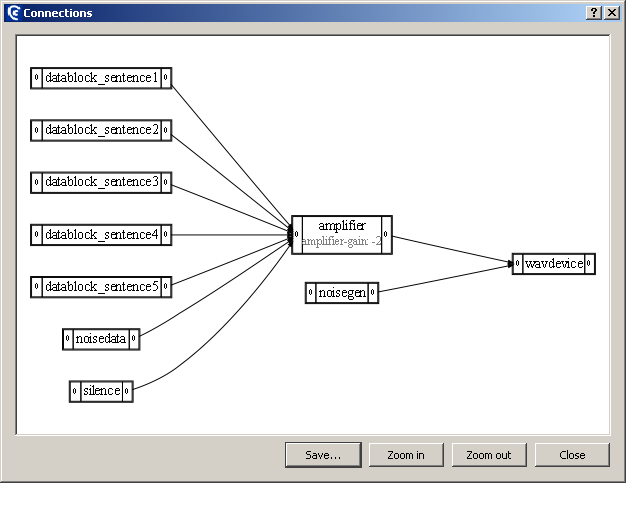
\includegraphics[width=0.8\textwidth]{connectionswindow.png}
 \caption{The connections window}
 \label{fig:connections}
\end{figure}

\subsection{Calibration}
\label{sec:Calibration}

\index{calibration}
In order to present any given stimulus at a known sound pressure level, a calibration gain is applied before the stimulus is played. Calibration is the process of measuring which calibration gain is necessary for a given stimulus to achieve a certain sound pressure level. 
Calibration parameters are set in the\element{calibration} element of the apx file. Here a \element{stimulus} ID and parameters to be calibrated are defined. Since the stimuli used in most experiments are short, it is often helpful to make a longer version of the stimulus for use during calibration. This stimulus must have it’s own \element{datablock} and \element{stimulus} element definitions. 
e.g:

\begin{lstlisting}

<datablock id="datablock_tone">
	<device>wavdevice</device>
	<uri>tone.wav</uri>
</datablock>

<datablock id="datablock_tone_long_calibration">
            <device>wavdevice</device>
            <uri>tone_long_calibration.wav</uri>
</datablock>

<stimulus id="stimulus_tone">
	<datablocks>
	<sequential>
		<datablock id="datablock_tone"/>
	</sequential>
	</datablocks>
	<variableParameters></variableParameters>
	<fixedParameters></fixedParameters>
</stimulus>

<stimulus id="stimulus_tone_long_calibration">
            <datablocks>
                <sequential>
                    <datablock id="datablock_tone_long_calibration "/>
                </sequential>
            </datablocks>
            <variableParameters></variableParameters>
            <fixedParameters></fixedParameters>
        </stimulus>

<calibration profile="Calibprofile_HIB">
        <stimuli>
            <stimulus id="stimulus_calibration_tone"/>
<stimulus id="stimulus_calibration_noise"/>
        </stimuli>
        <parameters>
            <parameter id="gainid_amp_tone">
                <targetamplitude>30</targetamplitude>
                <calibrationamplitude>80</calibrationamplitude>
                <mute>-150</mute>
                <min>-100</min>
                <max>100</max>
            </parameter>
            <parameter id="gainid_amp_noise">
                <targetamplitude>15</targetamplitude>
                <calibrationamplitude>80</calibrationamplitude>
                <mute>-150</mute>
                <min>-100</min>
                <max>100</max>
            </parameter>
        </parameters>
    </calibration>

\end{lstlisting}

The parameter to be calibrated is usually a gain parameter for an amplifier element. In the example there are two stimuli that need to be calibrated. The stimuli have datablock ID’s \id{stimulus_tone} and \id{stimulus_noise}. Since the stimuli are derived from different datablocks and different WAV files, they must be calibrated separately. For this reason, the datablocks are connected to separate amplifier elements with IDs \id{ampid\_sinusoid\_F250} and \id{ampid\_TENnoise}. In this example, these two amplifier gain parameters are calibrated.

Calibration consists of a GUI for calibrating parameters and saving and applying
calibration results. Any stimulus defined in the experiment files can be used as a calibration stimulus.

Typically, calibration is the process of measuring which value of
a digital parameter corresponds to a certain physical magnitude ,
e.g., determining which internal amplification is necessary for a
given wave file to achieve a certain sound pressure level.

\apex provides a GUI to ease calibration (figure~\ref{fig:calibration}).
\apex can only calibrate parameters, i.e., it can set a parameter
to a certain value such that the resulting physical magnitude is
the one defined in the experiment file in the
\element{calibration} element.

Because often the same calibration is useful for a set of
experiment files, calibrations are stored under so-called
\emph{calibration profiles}. The calibration profile to be used
must be specified in the \element{calibration} element. For
example if multiple experiment files are used for speech in noise
tests, the calibration profile could be \xml{SpeechInNoise}.

As it is possible to use \apex on the same computer with the same
experiment files and calibration profile in different contexts (e.g., different types of
headphones, which have different calibration settings), \apex
makes use of the concept \emph{hardware setup}. A hardware setup
associates a label to a certain set of hardware devices. The
current hardware setup can be selected at runtime, i.e., cannot be
specified in the experiment file.

If \element{calibration} is defined in the experiment file and the
calibration profile has not been calibrated before for the current
hardware setup, the calibration window will be shown at the start
of the experiment. 


If the calibration profile was calibrated before, but you wish to
recalibrate or change the current hardware setup, select
\emph{Recalibrate} from the menu, select \emph{Manage profiles}
and add the desired label for the current hardware configuration,
eg. ``RME + headphones'', and click \textbf{Add} and \textbf{OK}.
This configuration will also appear in the \apex window in the
lower right hand corner. Under \textbf{Details...} the different
calibration profiles that have been calibrated before will be
shown (figure~\ref{fig:calibrationprofiles}).

On the left hand side of the main calibration window the
parameters to be calibrated are shown (as specified in the
\element{calibration} element in the experiment file). In this
example the parameter \id{cardgain} is calibrated, i.e. the gain
of the sound card. First allow the calibration stimulus ample time
to be able to measure an accurate value with a measuring device or
use the averaging function of the device. Enter the measured
amplitude (in \textbf{Measured amplitude}) and click on
'\textbf{Correct output parameter}'. Repeat until the intended and
measured values are the same. To save the result, click
\textbf{apply}, and click on the OK button.  \apex will store this
profile and retrieve it each time it is used.


Important
\begin{itemize}

\item Remember to check whether the correct \emph{Hardware setup}
is selected when starting an experiment. \apex will always use the
hardware setup used in the previous experiment unless otherwise
specified.

\item \textbf{Apply} and \textbf{OK}. Each calibrated parameter
needs to be saved by clicking on Apply and after all parameters
are calibrated clicking on OK at the bottom of the dialog.
\end{itemize}

It can be of interest to calibrate at a higher level than the
desired stimulation level, to avoid interference of background
noise. If a yellow message appears, the signal has clipped.

\textbf{Important:} Calibration values are stored as a value of a parameter for a combination of calibration parameter ID, calibration profile name, and hardware setup. When APEX opens an experiment file with a calibration section, it will search an internal database for a value corresponding to this combination. The database is stored in the Windows registry or in a text file under \filename{\~/.config} in Linux. By default the database is specific for the current user. If you want to share calibration values across users, you need to make a profile global using the \filename{calibrationadmin} tool. \todo{explain more?}

Calibration values can be exported and imported to transport them across computers, or simply store them for future reference. This feature is available in the manage hardware setups screen. \todo{explain more?}


\begin{figure}
 \centering
 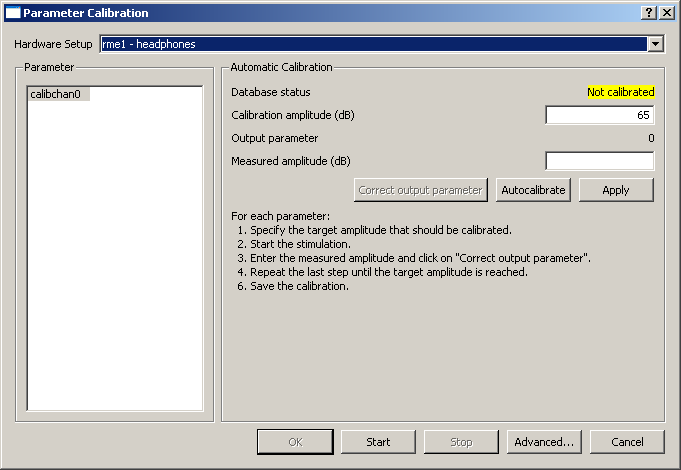
\includegraphics[width=\textwidth]{calibrationwindow.png}
 \caption{The calibration window}
 \label{fig:calibration}
\end{figure}


\begin{figure}
 \centering
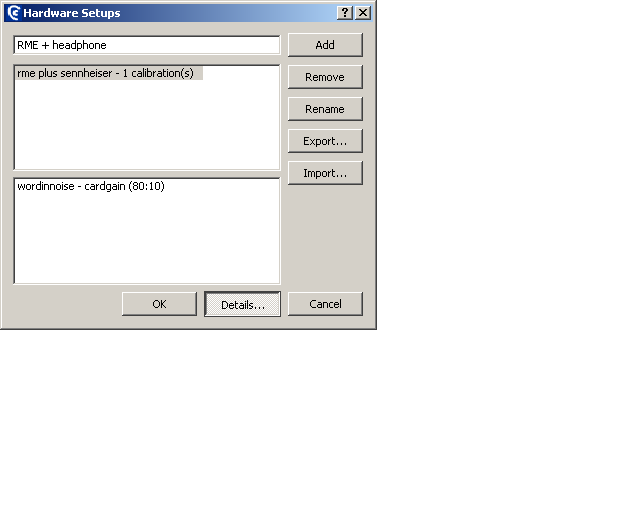
\includegraphics[width=0.8\textwidth]{calibrationwindow2.png}
 \caption{The calibration window showing \emph{Manage profiles}}
 \label{fig:calibrationprofiles}
\end{figure}
\label{sec:Calibration}


 \index{calibration}


\subsection{Results}
\label{sec:Results}


\index{results}

After completion of the experiment a file containing results can be saved to disk. The default results file is in XML and it has the extension \textbf{.apr}. It contains all the
information about the course of the completed experiment(e.g. number of reversals/trials, mean of reversals/trials in case of an adaptive procedure). 
APEX automatically assigns a default name to the results file. Namely, it append \textbf{-results }to the name of the experiment file (e.g. gapdetection-results.apr). APEX will never overwrite an existing results file, but will append a number to the results file in case of an existing results file (e.g. gapdetection-results-1.apx). The subjects name can be appended automatically to the suggested results file by specifying it in the \textbf{<subject/>} element. This is typically modified at the beginning of an experiment using an interactive entry (see section~\ref{sec:Interactive}).

e.g.:

\begin{lstlisting}
<results>
  <subject>John Doe</subject>
</results>
\end{lstlisting}

Please read section~\ref{chap:Results} for more information about displaying and analysing results.

\subsection{Interactive}
\index{Interactive}

\label{sec:Interactive}

Interactive allows the experimenter to modify certain aspects of
the experiment file right before the experiment is started using a
GUI.


\begin{itemize}
\item \element{Entry}
\end{itemize}

\subsection{General}
General defines some general parameters.

\label{sec:General}
\begin{itemize}
\item \element{show_results}

\item \element{saveprocessedresults}
\end{itemize}
\index{General}

\section{Parameters}
\index{parameters}

There are two types of parameters:
\begin{description}

\item [fixed parameter:] a fixed parameter is a property of a
stimulus. It cannot be changed by \apex at runtime and is defined
when the experiment file is created. It can be used by the
procedure to select a stimulus from a list, it can be shown on the
screen or it can be used as a piece of information when analyzing
results

\begin{lstlisting}
<stimuli>
    <fixed_parameters>
      <parameter id="gap"/>
    </fixed_parameters>

    <stimulus id="stimulus1" >
      <datablocks>
        <datablock id="gwith5msinterval" />
      </datablocks>
      <fixedParameters>
            <parameter id="gap">5</parameter>
      </fixedParameters>
    </stimulus>
    ....
</stimuli>
\end{lstlisting}

Fixed parameters are often used by adaptive procedures. If a
certain fixed parameter is selected to be adapted by a procedure,
the stimulus to be presented will be selected using that fixed
parameter. The stimuli are selected amongst those listed in the
current trial. In this example the duration of the gap is varied
in a gap detection task.

 \item [variable parameter:] a variable parameter is a
property of an object of which the value can be changed at
runtime. Variable parameters can be set by various \apex modules.
Examples of modules that can define variable parameters are
AdaptiveProcedure, Calibrator and Screen. Variable parameters can
also be defined for a Stimulus. If a stimulus description contains a
variable parameter, it will be set just before the stimulus is
presented. Examples of modules that can have variable parameters
(to be set by another module) are Filter, Controller and Device.
\end{description}.

\begin{lstlisting}

 <stimuli>
  <fixed_parameters/>
   <stimulus id="stimulus0">
      <description>Stimulus0</description>
      <datablocks>
        <datablock id="datablock0"/>
      </datablocks>
      <variableParameters>
        <parameter id="speaker">3</parameter>
        </variableParameters>
        <fixedParameters/>
    </stimulus>
</stimuli>

\end{lstlisting}


\label{sec:Parameters}

A variable stimulus parameter, is a parameter that will be set
elsewhere just before the stimulus is sent to the device. Take care that a variable parameter is not set by different modules and/or a stimulus, as the resulting behaviour is undefined. 

e.g. In examples 1 and 2 the gain of an amplifier is made a
variable parameter by assigning it ID \id{gain}


\subsection{Apexconfig}
\label{apexconfig}


The \filename{apexconfig.xml} file is a configuration file that
applies to all experiments. It is stored in the folder
\filename{config}, under the main \apex folder. It includes common
names of sound cards and drivers and prefixes that can be referred
to from any experiment file.

If the \filename{apexconfig.xml} is not defined for the current system user
the one in the \apex folder will be used. It is, however, also possible to have
an \filename{apexconfig.xml} file per user. To add an
\filename{apexconfig.xml} file for a specific user, log in as the
user, and copy the apexconfig.xml file to the folder
\filename{C:/Users/LoginName/Application Data/ExpORL}. If the file
\filename{apexconfig.xml} is present in the latter folder, it will
override the \filename{apexconfig.xml} file in the config folder
under main \apex directory. \apex can automatically make this copy when you click the "edit apexconfig file" option in the help menu.

\index{apexconfig}

\section{Using prefixes}

When specifying a prefix in an experiment file (e.g. in
\element{datablocks} or \element{screens}), it is possible, but
not necessary to write out the entire path in the XML file. This
path can also be defined once in the \filename{apexconfig.xml}
file located in the directory \filename{config}.

In other words, a prefix can be specified inline (i.e.: as the
content of the \element{uri_prefix} element) or by specifying the
ID of a prefix in the \apex config file and setting attribute
\attribute{source} to \filename {apexconfig}. You can specify a
complete \element {uri}or part of it.


A relative path given in the \element{uri_prefix} element is
always relative to the path of the experiment file. Since \apex
knows the location of the experiment file, only the folder
containing the wave files (and pictures) must be specified. If for
example the experiment file resides in
\filename{c:/temp/files/experiment.apx}, the prefix \xml{../..}
will point to \filename{c:/temp}.

In the experiment file, it is possible to specify the prefix as a relative path, relative to the location of the apex experiment, as follows:

\begin{lstlisting}
   <uri_prefix>../stimuli</uri_prefix>
\end{lstlisting}

Alternatively, it is possible to specify it as:

\begin{lstlisting}
<uri_prefix source="apexconfig">speechmaterials</uri_prefix>
\end{lstlisting}

The prefix \emph{"speechmaterials"} that you are using in the experiment file is defined in \filename{apexconfig.xml}. Sometimes it is useful to make your own apexconfig file (see section~\ref{sec:apexconfig}). This way, you can create several prefixes that for example refer to a folder containing all your stimuli (several speech materials, noise, modulated stimuli etc.) You can link your prefix with the absolute or relative path of the folder as follows: \\

\begin{lstlisting}
<prefix id="regression">file:../stimuli</prefix>
\end{lstlisting}

It is good practice to avoid using absolute paths in experiment files, as this makes your experiments portable to other computers. 

\label{sec:prefixes}

\index{prefixes}

\index{uri prefix}


\chapter{Examples}
\label{chap:Examples}

In this chapter we describe 4 examples: 1) a closed-set
identification task, 2) an adaptive speech in noise identification
task, and 3) an adaptive just noticeable difference task (gap
detection), and 4) same as 3, but modified to the attention span
and interest of young children. Each example consists of 1) a
general description, 2) the concept, and 3) the implementation in
XML.

It is advised to run the experiment before reading the details.
The experiment files are stored in the \apex directory under
\filename{examples/manual} in the \apex folder, together with
sound files and figures of the respective experiments. Note again:
if the experiment file has the extension ``.apx'' it remains an
XML file that can be edited with OxygenXML. The results file will
automatically have the extension ``.results''. \textbf{(needs to
be done)}.


\section{Overview of examples provided with APEX}

\subsection{calibration}
\subsubsection{calibration/calibration.apx}
\begin{description}
\item[Short] 
 Simple calibration use
\item[Description] 
 The experiment shows how to calibrate using the calibration screen. You can calibrate the left and right channel seperately.
\item[How] 
 Use the calibration element with a calibration profile and an id for each channel (left and right)
\end{description}

\subsubsection{calibration/calibration-automatic-bk2250.apx}
\begin{description}
\item[Short] 
 example of automatic calibration with B\&K SLM 2250 plugin
\item[Description] 
 calibrate left and right ear at the start of the experiment
\item[How] 
 The \textless{}soundlevelmeter\textgreater{} block specifies how to use the sound level meter. If the sound level meter is not found, the regular calibration dialog is shown.
\end{description}

\subsubsection{calibration/calibration-automatic-dummyslm.apx}
\begin{description}
\item[Short] 
 example of automatic calibration with dummy SLM plugin
\item[Description] 
 Allow to experiment with automatic calibration without having a sound level meter handy
\item[How] 
 The \textless{}soundlevelmeter\textgreater{} block specifies how to use the sound level meter.
\end{description}

\subsubsection{calibration/calibration-automatic-localisation.apx}
\begin{description}
\item[Short] 
 Automatic calibration using interface to sound level meter
\item[Description] 
 13-loudspeaker sound source localisation experiment, with automatic calibration through the interface to the B\&K SLM2250 Sound Level Meter
\item[How] 
 Each channel of the sound card has a gain. These gains are specified in the \textless{}calibration\textgreater{} element. Here the \textless{}soundlevelmeter\textgreater{} block specifies how to use the sound level meter. If the sound level meter is not found, the regular calibration dialog is shown.
\end{description}

\subsubsection{calibration/calibration-connections.apx}
\begin{description}
\item[Short] 

\item[Description] 

\item[How] 

\end{description}

\subsection{childmode}
\subsubsection{childmode/childmode-car-full.apx}
\begin{description}
\item[Short] 
 Shows use of child mode: intro and outro movies, child panel
\item[Description] 
 The experiment starts after a silent introductory movie. The child needs to find the animal in one of the three cars. One car has a different sound than the two other cars.
\item[How] 
 Flash elements are introduced that read movie files with extension .swf
\end{description}

\subsubsection{childmode/childmode-extramovies.apx}
\begin{description}
\item[Short] 
 Demonstration of extra movies (snail movie)
\item[Description] 
 The experiment starts after a silent introductory movie. The child needs to find the stimulus in one of the three snails. One snail has a different sound than the two other snails. Childfriendly feedback is provided.
\item[How] 
 Flash elements of snails
\end{description}

\subsubsection{childmode/childmode-full.apx}
\begin{description}
\item[Short] 
 Shows use of child mode: intro and outro movies, child panel, progressbar, shortcuts.
\item[Description] 
 The experiment starts after a silent introductory movie. The child needs to find the stimulus in one of the three eggs. One egg has a different sound than the two other eggs. The progressbar and feedback are also childfriendly.
\item[How] 
 Flash elements are introduced that read movie files with extension.swf, child panel activated by \textless{}panel\textgreater{} in \textless{}childmode\textgreater{} (\textless{}screens\textgreater{}) + button shortcuts are introduced (button 1 = 1, button 2 = 2, button 3 = 3)
\end{description}

\subsubsection{childmode/childmode-full-L34.apx}
\begin{description}
\item[Short] 
 Shows use of child mode: intro and outro movies, child panel, progressbar for L34
\item[Description] 
 The experiment starts after a silent introductory movie. The child needs to find the stimulus in one of the three eggs. One egg has a different sound than the two other eggs.  The progressbar and feedback are also childfriendly.
\item[How] 
 Flash elements, L34 implementation in \textless{}devices\textgreater{}
\end{description}

\subsubsection{childmode/childmode-justmovies.apx}
\begin{description}
\item[Short] 
 Shows use of child mode: without intro and outro movies, but with the normal panel
\item[Description] 
 The child needs to find the stimulus in one of the three eggs. One egg has a different sound than the two other eggs. The same progressbar is used as in adult experiments, feedback is childfriendly.
\item[How] 
 Flash elements, same panel as adult experiments (no childmode selected in \textless{}screens\textgreater{})
\end{description}

\subsubsection{childmode/childmode-movies+intro.apx}
\begin{description}
\item[Short] 
 Shows use of flash movies, but without the actual childmode (no childpanel)
\item[Description] 
 The experiment starts after a silent introductory movie. The child needs to find the stimulus in one of the three eggs. The same progressbar is used as in adult experiments. Feedback is childfriendly.
\item[How] 
 flash elements, same panel as adult experiments (no \textless{}panel\textgreater{}reinforcement.swf\textless{}/panel\textgreater{} in childmode)
\end{description}

\subsubsection{childmode/childmode-nofeedback.apx}
\begin{description}
\item[Short] 
 Shows use of child mode without special feedback movies
\item[Description] 
 The experiment starts after a silent introductory movie. The child needs to find the stimulus in one of the three eggs. One egg has a different sound than the two other eggs.
\item[How] 
 Flash elements, no special feedback with flash elements provided
\end{description}

\subsubsection{childmode/childmode-noprogress.apx}
\begin{description}
\item[Short] 
 Shows use of child mode: intro and outro movies, but without the actual childmode (no childpanel)
\item[Description] 
 The experiment starts after a silent introductory movie. The child needs to find the stimulus in one of the three eggs. One egg has a different sound than the two other eggs. Feedback is childfriendly.
\item[How] 
 Flash elements, no panel or progressbar (\textless{}showpanel\textgreater{}false\textless{}/showpanel\textgreater{} and \textless{}progressbar\textgreater{}false\textless{}/progressbar\textgreater{})
\end{description}

\subsubsection{childmode/childmode-onlyscreen-normalpanel.apx}
\begin{description}
\item[Short] 
 Shows use of child mode: intro and outro movies, but with the normal panel
\item[Description] 
 The experiment starts after a silent introductory movie. The child needs to find the stimulus in one of the three eggs. One egg has a different sound than the two other eggs. The same progressbar is used as in adult experiments. Feedback is childfriendly.
\item[How] 
 Flash elements, same panel as adult experiments (no childmode selected in \textless{}screens\textgreater{})
\end{description}

\subsubsection{childmode/childmode-poll.apx}
\begin{description}
\item[Short] 
  Shows use of child mode: instead of waiting a specific time, 0 is specified as length for intro, outro and feedback, which makes apex wait for the movies to finish.
\item[Description] 
 The experiment starts after a silent introductory movie. The child needs to find the stimulus in one of the three eggs. One egg has a different sound than the two other eggs. The same progressbar is used as in adult experiments.
\item[How] 
 Flash elements, same panel as adult experiments (no childmode selected in \textless{}screens\textgreater{}), length of intro and outro is specified in \textless{}childmode\textgreater{}
\end{description}

\subsubsection{childmode/childmode-shortcuts.apx}
\begin{description}
\item[Short] 
 Shows use of child mode with shortcut keys
\item[Description] 
 The experiment starts after a silent introductory movie. The child needs to find the stimulus in one of the three eggs. One egg has a different sound than the two other eggs. The progressbar and feedback are also childfriendly.
\item[How] 
 Flash elements, button shortcuts are introduced (leftarrow = 1, downarrow = 2, rightarrow = 3)
\end{description}

\subsubsection{childmode/childmode-skipintrooutro.apx}
\begin{description}
\item[Short] 
 Shows use of child mode: intro and outro movies, but without the child panel; also has button shortcuts to skip the intro or outro movie
\item[Description] 
 The experiment starts after a silent introductory movie. The child needs to find the stimulus in one of the three eggs. One egg has a different sound than the two other eggs. Feedback is also childfriendly.
\item[How] 
 The F7 shortcut can be used to skip the intro and outro movies when \textless{}allowskip\textgreater{}true\textless{}/allowskip\textgreater{} in \textless{}general\textgreater{}. Flash elements, button shortcuts are introduced (leftarrow = 1, downarrow = 2, rightarrow = 3, 's' = skipping intro or outro movie),
\end{description}

\subsubsection{childmode/childmode-skipintrooutro-disabled.apx}
\begin{description}
\item[Short] 
 Skip intro or outro movie by hitting 's' on the keyboard is disabled.
\item[Description] 
 The experiment starts after a silent introductory movie. The child needs to find the stimulus in one of the three eggs. One egg has a different sound than the two other eggs. Feedback is childfriendly.
\item[How] 
 Flash elements, skipping is disabled by setting  \textless{}allowskip\textgreater{}false\textless{}/allowskip\textgreater{} in \textless{}general\textgreater{}
\end{description}

\subsubsection{childmode/childmode-snake-full.apx}
\begin{description}
\item[Short] 
 Shows use of child mode: intro and outro movies, child panel, progressbar
\item[Description] 
 The experiment starts after a silent introductory movie. The child needs to find the stimulus in one of the three snakes. One snake has a different sound than the two other snakes. The progressbar and feedback are also childfriendly.
\item[How] 
 Flash elements of snakes, child panel activated by \textless{}panel\textgreater{} in \textless{}childmode\textgreater{} (\textless{}screens\textgreater{})
\end{description}

\subsubsection{childmode/childmode-waitforstart.apx}
\begin{description}
\item[Short] 
 Shows use of child mode, with no shortcut keys and waiting for start before every trial
\item[Description] 
 The experiment starts after a silent introductory movie. The child needs to find the stimulus in one of the three eggs. One egg has a different sound than the two other eggs. The next trial is only presented after selecting Start from the Experiment menu or pressing F5.
\item[How] 
 Flash elements + \textless{}waitforstart\textgreater{} function in \textless{}general\textgreater{}
\end{description}

\subsection{connections}
\subsubsection{connections/connections-all-mixed-monostereo.apx}
\begin{description}
\item[Short] 
 The use of ALL connections
\item[Description] 
 Monaural presentations of digit 1. Level is changed by clicking the buttons quieter and louder
\item[How] 
 Connections defines how the different datablocks and filters are routed to the output device
\end{description}

\subsubsection{connections/connections-byname.apx}
\begin{description}
\item[Short] 
 Try to autoconnect a stereo wavfile to a mono wavdevice by name
\item[Description] 
 Digits are presented dichotically, you can give a verbal response
\item[How] 
 Connections are used to route different datablocks and filters to an output device
\end{description}

\subsubsection{connections/connections-byregexp.apx}
\begin{description}
\item[Short] 
 Try to autoconnect a stereo wavfile to a mono wavdevice using mode=regexp
\item[Description] 
 Dichotic presentation of digits, you can give a verbal response
\item[How] 
 Connections are used to route different datablocks and filters to an output device
\end{description}

\subsubsection{connections/connections-bywildcard.apx}
\begin{description}
\item[Short] 
 Try to autoconnect a stereo wavfile to a mono wavdevice using mode=wildcard
\item[Description] 
 Dichotic presentation of digits, you can give a verbal response
\item[How] 
 Connections are used to route different datablocks and filters to an output device
\end{description}

\subsubsection{connections/connections-negativechannel.apx}
\begin{description}
\item[Short] 
 Test the use of channel -1
\item[Description] 
 If something is connected to channel -1 of the output device, it should be ignored, no output when button wrong is clicked
\item[How] 
 Connections are used to route filters to output devices
\end{description}

\subsection{controller}
\subsubsection{controller/controller-plugincontroller.apx}
\begin{description}
\item[Short] 
 Plugincontroller
\item[Description] 
 Gain of plugin controller varies according to user input
\item[How] 
 the democontroller is used here to demonstrate how a plugin controller can be implemented.
\end{description}

\subsubsection{controller/osccontroller.apx}
\begin{description}
\item[Short] 
\item[Description] 
\item[How] 
\end{description}

\subsubsection{controller/osccontroller\_avatar.apx}
\begin{description}
\item[Short] 
\item[Description] 
\item[How] 
\end{description}

\subsection{datablocks}
\subsubsection{datablocks/datablocks-combination.apx}
\begin{description}
\item[Short] 
 Combination of datablocks using sequential and simultaneous
\item[Description] 
  Play datablocks similtaneously and sequentially
\item[How] 
 Using the \textless{}simultaneous\textgreater{} and \textless{}sequential\textgreater{} tags in \textless{}stimulus\textgreater{}, datablocks can be organised and reused.
\end{description}

\subsubsection{datablocks/datablocks-loop.apx}
\begin{description}
\item[Short] 
 Use the same datablock multiple times in a stimulus
\item[Description] 
 The datablock wavfile "één" is played twice within one stimulus
\item[How] 
 set the number of replications of the datablock by setting the number of the loop, here it is \textless{}loop\textgreater{}2\textless{}/loop\textgreater{}
\end{description}

\subsubsection{datablocks/datablocks-nodevice.apx}
\begin{description}
\item[Short] 
 demonstration of omission of device in datablock
\item[Description] 
 When there is only one device in the experiment, it does not need to be explicitly mentioned in each datablock.
\item[How] 
 APEX will automatically assign the device to each datatblock
\end{description}

\subsubsection{datablocks/datablocks-repeat.apx}
\begin{description}
\item[Short] 
 Use the same datablock multiple times in a stimulus
\item[Description] 
 The datablock wavfile "één" is played four times within one stimulus
\item[How] 
 sequential datablocks within stimulus1
\end{description}

\subsubsection{datablocks/datablocks-silence.apx}
\begin{description}
\item[Short] 
 Combination of silence and signal for 1 stimulus presentation
\item[Description] 
 The stimulus in this example contains first silence (a delay) before you hear "één"
\item[How] 
 Use sequential datablocks that include silence and wavfile/signals, e.g. also possible to put silence datablocks after the wavfile
\end{description}

\subsubsection{datablocks/datablocks-simultaneous.apx}
\begin{description}
\item[Short] 
 Play datablocks simultaneously
\item[Description] 
 Demonstrate the use of simultaneous datablocks in a stimulus
\item[How] 
 When datablocks are listed in the \textless{}simultaneous\textgreater{} element in \textless{}stimulu\textgreater{} they are played simultaneously
\end{description}

\subsection{filters}
\subsubsection{filters/filters-amplifier-defaultparameters.apx}
\begin{description}
\item[Short] 
 Show amplifier default parameters
\item[Description] 
 the stimulus wd1.wav is played in the left ear, when you click the button 'play with default parameters', the stimulus is played again with the same gain (=0) (10 trials)
\item[How] 
 fixed\_parameters
\end{description}

\subsubsection{filters/filters-amplifier-setgain.apx}
\begin{description}
\item[Short] 
 Adapting device parameters: gain of device varies according to user input
\item[Description] 
 the stimulus wd1.wav and noise are played simultaneously in the left ear, when you click the button 'higher'/'lower', the stimulus and the noise are played again with a different gain for the noise (= gain + 2/- 2, see output box 'parameterlist')
\item[How] 
 adaptiveProcedure: gain is adjusted with stepsize = 2
\end{description}

\subsubsection{filters/filters-complexprocessing.apx}
\begin{description}
\item[Short] 
 More complex processing, can be used for testing skips - 2 noise stimuli (sinus \& wivineruis.wav) with different gains (filters)
\item[Description] 
 When you click on 'wrong' you hear in both ears two noise stimuli and in the left ear 2 times a sentence, the same happens when you click on the 'wrong' button again
\item[How] 
 trainingProcedure, creating a sinus as noise-stimulus
\end{description}

\subsubsection{filters/filters-dataloop-2simultaneous.apx}
\begin{description}
\item[Short] 
 Shows use of dataloop generator : uses the same datablock twice (for 2 different dataloops)
\item[Description] 
 When you click on the button 'correct/wrong', in both ears a noise stimulus is played and in the left ear 'one-two'(=stimulus1)/'silence-two'(=stimulus2) is presented - Dataloop: playing noise and according to the users input (correct/wrong) stimulus1 or stimulus2 is presented
\item[How] 
 2 dataloops: noise for trial1 and trial2
\end{description}

\subsubsection{filters/filters-dataloop.apx}
\begin{description}
\item[Short] 
 Shows use of dataloop generator - wivineruis.wav should play !not! continuously over trials (see filters - noisegen - apex:dataloop)
\item[Description] 
 When you click on the button 'wrong/correct', in both ears a noise stimulus is played and in the left ear 'silence-two(twee)'(=stimulus2)/'one-two(een-twee)'(=stimulus1) is presented
\item[How] 
 trainingProcedure - dataloop generator - continuous: false
\end{description}

\subsubsection{filters/filters-dataloop-continuous.apx}
\begin{description}
\item[Short] 
 Shows use of dataloop generator - wivineruis.wav should play continuously over trials (see filters - noisegen - apex:dataloop)
\item[Description] 
 The noise is playing continuously over trials. When you click on the button 'dataloop - silence/dataloop - 1', in both ears a noise stimulus is played and in the left ear 'silence-two(twee)'(=stimulus2)/'one-two(een-twee)'(=stimulus1) is presented
\item[How] 
 trainingProcedure - dataloop generator - continuous: true
\end{description}

\subsubsection{filters/filters-dataloop-jump.apx}
\begin{description}
\item[Short] 
 Shows use of jump parameter of dataloop generator
\item[Description] 

\item[How] 

\end{description}

\subsubsection{filters/filters-dataloop-randomjump.apx}
\begin{description}
\item[Short] 

\item[Description] 

\item[How] 

\end{description}

\subsubsection{filters/filters-noisegen-setgain.apx}
\begin{description}
\item[Short] 
 Basegain of noise: 0 - Aapting device parameters - gain of device varies according to user input
\item[Description] 
 Noise and a stimulus (one-een) are presented simultaneously in the left ear, when you click on 'higher/lower', you hear again the noise and stimulus in the left ear but the gain of the noise is adjusted with +2/-2 (=stepsize, see output box)
\item[How] 
 adaptiveProcedure - stepsize of gain - adapt\_parameter (Procedure) - continuous:true
\end{description}

\subsubsection{filters/filters-plugin.apx}
\begin{description}
\item[Short] 

\item[Description] 
 example already somewhere else as well!
\item[How] 

\end{description}

\subsubsection{filters/filters-plugin-matlabfilter.apx}
\begin{description}
\item[Short] 
 Example using the matlabfilter plugin.
\item[Description] 
  The plugin will use matlab to process data, one buffer at a time. Note that you should make sure your system can find the Matlab eng library.
\item[How] 
 \textless{}plugin\textgreater{}matlabfilter\textless{}/plugin\textgreater{} in \textless{}filters\textgreater{}.
\end{description}

\subsubsection{filters/filters-plugin-scamblespectrumfilter.apx}
\begin{description}
\item[Short] 
 Demonstrate scramblespectrum filter
\item[Description] 
 The scramblespectrum filter will randomize the spectrum to reduce monaural spectral cues in a localisation experiment
\item[How] 
 parameters to the scramblespectrumfilter are specified in \textless{}filter\textgreater{}
\end{description}

\subsubsection{filters/filters-plugin-scamblespectrumfilter\_calibration.apx}
\begin{description}
\item[Short] 

\item[Description] 

\item[How] 

\end{description}

\subsubsection{filters/filters-pulsegen.apx}
\begin{description}
\item[Short] 
        Shows synchronisation for L34 using a soundcard pulse
\item[Description] 
 When you click on send, a pulse is presented in your left ear
\item[How] 
 filters: generator makes a soundcard pulse =\textgreater{} 2 channels of stereo file are mixed into output ch 0, the pulse goes to ch 1 (left ear)
\end{description}

\subsubsection{filters/filters-sinegenerator.apx}
\begin{description}
\item[Short] 
 Test of setting frequency parameter of sine generator - frequency of sinus varies according to user input
\item[Description] 
 A sinus is playing in the left ear when you click on one of the 3 buttons. If you click on 100Hz/1000Hz/defaults, the frequency of the sinus changes to 100Hz/1000Hz/10 000Hz.
\item[How] 
 filter: 1 generator: sinus (10 000Hz) - 3 stimuli: 3x silence with adjusted parameters (frequency: 100Hz/1000Hz/no change) -  continuous: false
\end{description}

\subsubsection{filters/filters-sinegen-setfrequency.apx}
\begin{description}
\item[Short] 
 Regression test for adapting device parameters - gain of device varies according to user input
\item[Description] 
 A sinus is played in the left ear (sinus is played continuously over trials), when you click the button 'higher'/'lower', the sinus is played again with a different frequency for the sinus (= frequency + 100Hz/- 100Hz, see output box 'parameterlist')
\item[How] 
 adaptiveProcedure: frequency (adapt\_parameter) is adjusted with stepsize = 100Hz - datablock/stimulus: silence
\end{description}

\subsubsection{filters/filters-sinegen-setgain.apx}
\begin{description}
\item[Short] 
 Regression test for adapting device parameters - gain of device varies according to user input
\item[Description] 
 A sinus is played in the left ear. The sinus is played continuously over trial but when you click on 'higher/lower' the sinus is played again but the gain of the sinus is adapted with +5/-5 dB.
\item[How] 
 adaptiveProcedure - datablock/stimulus: silence - filter: generator: sinus - continuous: true - adapt\_parameter: gain - (!basegain has to be low enough otherwise there is clipping!)
\end{description}

\subsubsection{filters/filters-singlepulse-defaultparameters.apx}
\begin{description}
\item[Short] 
        Shows synchronisation  using a soundcard pulse
\item[Description] 
 When you click on 'play with default parameters', a pulse is presented in your left ear simultaneously with a stimulus (wd1.wav - een/one)
\item[How] 
 datablock/stimulus + filter: generator makes a soundcard pulse (negative polarity)
\end{description}

\subsubsection{filters/filters-singlepulse-polarity.apx}
\begin{description}
\item[Short] 
        Shows synchronisation for L34 using a soundcard pulse with a negative polarity (filter - pulsegen)
\item[Description] 
 When you click on send, a pulse is presented in your left ear and a stimulus (datablock: \_Input44\_2.wav) is presented in your right ear
\item[How] 
 filters: generator makes a soundcard pulse with a negative polarity
\end{description}

\subsubsection{filters/filters-vocoder.apx}
\begin{description}
\item[Short] 
 Demonstration of vocoder plugin.
\item[Description] 
 Play a sentence either vocoded or unvocoded
\item[How] 
 A vocoder-plugin filter has been added in the connections.
\end{description}

\subsubsection{filters/filters-wavamplifier.apx}
\begin{description}
\item[Short] 
 Regression test for training procedure - Output: number according to last input
\item[Description] 
 When you click on the button 'play': in the left ear/channel: "een", is presented and in the right ear/channel: "twee", 20dB louder compared to the left ear, is presented.
\item[How] 
 filter: amplifier =\textgreater{} basegain (-10) + gain left channel(-10)/right channel(+10)
\end{description}

\subsubsection{filters/filters-wavfadeincos.apx}
\begin{description}
\item[Short] 
 Regression test for fader (begin/end of stimulus is not abrupt)
\item[Description] 
 When you click on the button 'play fade/play NO fade', in both ears a sinus is presented with at the beginning of the stimulus a fade-in/NO fade-in (click)
\item[How] 
 filter: fader in begin (cosine) =\textgreater{} length: 400ms, direction: in (fade-in: begin of stimulus)
\end{description}

\subsubsection{filters/filters-wavfadeinlin.apx}
\begin{description}
\item[Short] 
 Regression test for fader (begin/end of stimulus is not abrupt)
\item[Description] 
 When you click on the button play fade/play NO fade', in both ears a sinus is presented with at the beginning of the stimulus a fade-in/NO fade-in (click)
\item[How] 
 filter: fader(linear) =\textgreater{} length: 400ms, direction: in (fade-in: begin of stimulus)
\end{description}

\subsubsection{filters/filters-wavfadeoutcos.apx}
\begin{description}
\item[Short] 
 Regression test for fader (begin/end of stimulus is not abrupt)
\item[Description] 
 When you click on the button 'play fade/play NO fade', in both ears a sinus is presented with at the end of the stimulus a fade-out/NO fade-in (click)
\item[How] 
 filter: fader(cosine) =\textgreater{} length: 400ms, direction: out (fade-out: end of stimulus)
\end{description}

\subsubsection{filters/filters-wavfadeoutlin.apx}
\begin{description}
\item[Short] 
 Regression test for fader (begin/end of stimulus is not abrupt)
\item[Description] 
 When you click on the button 'play fade/play NO fade', in both ears a sinus is presented with at the end of the stimulus a fade-out/NO fade-in (click)
\item[How] 
 filter: fader(linear) =\textgreater{} length: 400ms, direction: out (fade-out: end of stimulus)
\end{description}

\subsection{general}
\subsubsection{general/general-autosave.apx}
\begin{description}
\item[Short] 
 Automatically save results to apr-file after experiment
\item[Description] 
 Closed-set identification task with automatic saving of results
\item[How] 
 General - autosave
\end{description}

\subsubsection{general/general-exitafter.apx}
\begin{description}
\item[Short] 
 Exit experiment when finished
\item[Description] 
 Closed-set identification task, exit after finish
\item[How] 
 General - exitafter=true
\end{description}

\subsubsection{general/general-prefix-absolutepath.apx}
\begin{description}
\item[Short] 
 Get the datablock prefix from the absolute path
\item[Description] 
 Closed-set identification task
\item[How] 
 datablocks uri\_prefix full path
\end{description}

\subsubsection{general/general-prefix-frommainconfig.apx}
\begin{description}
\item[Short] 
   Get the datablock prefix from the main configfile
\item[Description] 
 Closed-set identification task
\item[How] 
 source=apexconfig
\end{description}

\subsubsection{general/general-prefix-invalid.apx}
\begin{description}
\item[Short] 
 Get the datablock prefix from the main configfile
\item[Description] 
 Invalid prefix id specified: wavfile not found wd1.wav
\item[How] 
 source=apexconfig
\end{description}

\subsubsection{general/general-scriptparameters.apx}
\begin{description}
\item[Short] 
 Demonstrate the use of general/scriptparameters
\item[Description] 
 Digits 1-7 are presented monaurally, you can click on a button to go to the next one
\item[How] 
 Scriptparameters - name=path, scriptparameters.js needed
\end{description}

\subsubsection{general/general-showresults.apx}
\begin{description}
\item[Short] 
 Show results after experiment
\item[Description] 
 When the experiment is finished and the results are saved, you can choose to see the results
\item[How] 
 Results - showafterexperiment=true
\end{description}

\subsubsection{general/general-xmlerror.apx}
\begin{description}
\item[Short] 
 Error in XML file
\item[Description] 

\item[How] 

\end{description}

\subsection{interactive}
\subsubsection{interactive/invalid-entry.apx}
\begin{description}
\item[Short] 
 Change small parameter right before the start of the experiment
\item[Description] 
 GUI is shown with the element to be changed
\item[How] 
 Interactive
\end{description}

\subsubsection{interactive/setgain.apx}
\begin{description}
\item[Short] 
 GUI to change some settings right before the experiment
\item[Description] 
 GUI appears to set/change some settings
\item[How] 
 Interactive
\end{description}

\subsubsection{interactive/subject.apx}
\begin{description}
\item[Short] 
 GUI to change some settings right before the experiment
\item[Description] 
 GUI appears to set/change some settings
\item[How] 
 The name of the subject, in \textless{}results\textgreater{}/\textless{}subject\textgreater{} is set from the interactive dialog that appears before the experiment is loaded.
\end{description}

\subsection{l34}
\subsubsection{l34/addinvalidfilter.apx}
\begin{description}
\item[Short] 
 Try to add wav filter to L34Device
\item[Description] 
 Since it is not possible to add a wav filter to an L34Device, an error occurs
\item[How] 
 see filters and device
\end{description}

\subsubsection{l34/bilateral.apx}
\begin{description}
\item[Short] 
 Test of synchronized bilateral CI setup
\item[Description] 
 Test whether the stimuli are given from the first, the second or both L34 devices
\item[How] 
 Including two L34 devices, stimuli can be presented stimultaneously
\end{description}

\subsubsection{l34/bilateral-singlepulse.apx}
\begin{description}
\item[Short] 
 Test of synchronized bilateral CI setup with pulse stimuli
\item[Description] 
 Test whether the stimuli are given from the first, the second or both L34 devices
\item[How] 
 Including two L34 devices, stimuli can be presented stimultaneously
\end{description}

\subsubsection{l34/invaliddatablock.apx}
\begin{description}
\item[Short] 
 Try to parse invalid datablock, should return error
\item[Description] 
 datablock does not exist in folder stimuli, running the experiment gives an error.
\item[How] 
 uri\_prefix is used to find stimuli, invalid.aseq does not exist
\end{description}

\subsubsection{l34/L34DummySync.apx}
\begin{description}
\item[Short] 
        Shows synchronisation for L34 using a soundcard pulse
\item[Description] 
         2 channels of stereo file are mixed into output ch 0, the pulse goes to ch 1
\item[How] 
 use dummyDeviceType and wavDeviceType and check connections
\end{description}

\subsubsection{l34/L34Sync.apx}
\begin{description}
\item[Short] 
        Shows synchronisation for L34 using a soundcard pulse
\item[Description] 
         2 channels of stereo file are mixed into output ch 0, the pulse goes to ch 1
\item[How] 
 use dummyDeviceType and wavDeviceType and check connections
\end{description}

\subsubsection{l34/loudness\_balancing.apx}
\begin{description}
\item[Short] 
 Loudness balancing between two stimulation CI electrodes
\item[Description] 
 Two signals are presented consecutively in the same CI, at two different stimulation electrodes. One electrode is the reference electrode and has a fixed current level, the comparison electrode has changing levels. The participant has to judge which signal is louder. An adaptive procedure is used to determine the balanced level.
\item[How] 
 Use of adaptiveProcedure, plugindatablocks, balancing.js needed
\end{description}

\subsubsection{l34/mapping1.apx}
\begin{description}
\item[Short] 
 Use default map with current units between 1 and 255
\item[Description] 

\item[How] 
 See defaultmap
\end{description}

\subsubsection{l34/mapping2.apx}
\begin{description}
\item[Short] 
 Use real map to check mapping
\item[Description] 

\item[How] 
 See defaultmap values
\end{description}

\subsubsection{l34/r126wizard.apx}
\begin{description}
\item[Short] 
 R126 is the clinical fitting software
\item[Description] 

\item[How] 
 Use \textless{}defaultmap\textgreater{} \textless{}from\_r126/\textgreater{}
\end{description}

\subsubsection{l34/rfgenxs-bilateral.apx}
\begin{description}
\item[Short] 
 Test of synchronized bilateral CI setup with an RFGenXS
\item[Description] 
 Test whether the stimuli are given on the first, the second or both channels
\item[How] 
 With an RFGenXS, stimuli can be presented stimultaneously
\end{description}

\subsubsection{l34/setvolume.apx}
\begin{description}
\item[Short] 
 Change volume of CI stimuli (send simple XML file to L34 device)
\item[Description] 
 Change the volume of the CI stimuli to 10,50,70 or 100 current units
\item[How] 
 Add variable parameter id=l34volume, see device: volume 100 is default
\end{description}

\subsubsection{l34/simpleaseq.apx}
\begin{description}
\item[Short] 

\item[Description] 

\item[How] 

\end{description}

\subsubsection{l34/simpleaseq-dummy.apx}
\begin{description}
\item[Short] 

\item[Description] 

\item[How] 

\end{description}

\subsubsection{l34/simpleaseq-examples.apx}
\begin{description}
\item[Short] 
 power-up test?
\item[Description] 

\item[How] 

\end{description}

\subsubsection{l34/simpleaseq-sp12.apx}
\begin{description}
\item[Short] 

\item[Description] 

\item[How] 

\end{description}

\subsubsection{l34/triggertest.apx}
\begin{description}
\item[Short] 

\item[Description] 

\item[How] 

\end{description}

\subsubsection{l34/wordsaseq.apx}
\begin{description}
\item[Short] 

\item[Description] 

\item[How] 

\end{description}

\subsection{manual}
\subsubsection{manual/closedsetword.apx}
\begin{description}
\item[Short] 
 Closed-set identification of words in noise with figures
\item[Description] 
 A word is presented in noise and the subject responds by clicking on one of the 4 figures on the screen, repeated 3 times. Initial SNR is set via interactive GUI.
\item[How] 
 full experiment
\end{description}

\subsubsection{manual/gapdetection.apx}
\begin{description}
\item[Short] 
 Gap detection
\item[Description] 

\item[How] 

\end{description}

\subsubsection{manual/gapdetectionchild.apx}
\begin{description}
\item[Short] 
 gap detection for children
\item[Description] 

\item[How] 

\end{description}

\subsubsection{manual/opensetidentification.apx}
\begin{description}
\item[Short] 
 Open set identification task
\item[Description] 
 A word is presented in noise and the subject responds by typing the word, repeated 3 times. Initial SNR is set via interactive GUI.
\item[How] 
 Full experiment
\end{description}

\subsubsection{manual/sentenceinnoise.apx}
\begin{description}
\item[Short] 
 Sentences in noise task
\item[Description] 
 A sentence is presented in noise, the subject responds verbally, the test leader can indicatie whether the response was correct or incorrect, repeated 4 times. Initial SNR is set via interactive GUI.
\item[How] 
 Full experiment
\end{description}

\subsubsection{manual/trainingprocedure.apx}
\begin{description}
\item[Short] 
 Training for constant procedure
\item[Description] 
 A stimulus is presented after the user had indicated the trial by pressing a button on the screen
\item[How] 
 apex:trainingProcedure
\end{description}

\subsection{parameters}
\subsubsection{parameters/parameters-connection-filter.apx}
\begin{description}
\item[Short] 
 Change the channel of a connection + stimulus has gain
\item[Description] 
 Click on the right (or left button) to hear the sound in your right ear (or left ear).
\item[How] 
 Training procedure, Fixed (stimulus) and variable parameters (channel) + possibility in code to change the gain of the stimuli with filter (amplifier)
\end{description}

\subsubsection{parameters/parameters-connection-soundcard.apx}
\begin{description}
\item[Short] 
 Change the channel of a connection using a parameter
\item[Description] 
 Click on the right (or left button) to hear the sound in your right ear (or left ear)
\item[How] 
 training procedure, Fixed (stimulus) and variable parameters (channel)
\end{description}

\subsubsection{parameters/parameters-device-allchannels.apx}
\begin{description}
\item[Short] 
 Change parameter (gain) of device channel
\item[Description] 
 gain of device varies in BOTH channels according to user input (1 button = louder, 1 button = quieter)
\item[How] 
 adaptive procedure, fixed (stimulus) and variable (gain) parameters, stepsize of 2 dB
\end{description}

\subsubsection{parameters/parameters-device-singlechannel.apx}
\begin{description}
\item[Short] 
 Change parameter (gain) of device channel
\item[Description] 
 Gain of device varies in LEFT channel according to user input (1 button = louder, 1 button = quieter)
\item[How] 
 Adaptive procedure, fixed (stimulus) and variable (gain) parameters, stepsize of 2 dB
\end{description}

\subsubsection{parameters/parameters-filter.apx}
\begin{description}
\item[Short] 
 Change parameter (gain) of device channel
\item[Description] 
 gain of device varies in BOTH channel according to user input (1 button = louder, 1 button = quieter) + gain is visible on the screen
\item[How] 
 adaptive procedure, fixed (stimulus) and variable (gain) parameters, stepsize of 2 dB, Parameterlists are introduced that show Left or Right gain on the screen
\end{description}

\subsubsection{parameters/parameters-filter-channel.apx}
\begin{description}
\item[Short] 
 Change parameter (gain) of device channel
\item[Description] 
 gain of device varies in RIGHT channel according to user input (1 button = louder, 1 button = quieter) + gain is visible on screen
\item[How] 
 adaptive procedure, fixed (stimulus) and variable (gain) parameters, stepsize of 2 dB, Parameterlists are introduced that show Left or Right gain on the screen
\end{description}

\subsubsection{parameters/parameters-filter-channel-probe.apx}
\begin{description}
\item[Short] 
  Change parameter (gain) of device channel
\item[Description] 
 gain of device varies in LEFT channel according to user input (1 button = louder, 1 button = quieter) + gain is visible on screen
\item[How] 
 adaptive procedure, fixed (stimulus) and variable (gain) parameters, stepsize of 10 dB, Parameterlists are introduced that show Left or Right gain on the screen. Additionally there is a probe filter that saves the output to disk.
\end{description}

\subsubsection{parameters/parameters-restore.apx}
\begin{description}
\item[Short] 
 Demonstrate restoring parameter values
\item[Description] 
 When a parameter is set from a stimulus, and subsequently a stimulus is played in which the parameter is not set, it should be restored to its default value
\item[How] 
 Parameter gain is set in stimulus1, and is not set in stimulus2. Therefore a gain of 0dB should be applied for stimulus2
\end{description}

\subsubsection{parameters/parameters-spinbox.apx}
\begin{description}
\item[Short] 
 Adjust noise manually while presenting speech and noise
\item[Description] 
 gain of noise varies in right channel according to user input (1 button = arrow up, 1 button = arrow down) while the stimulus stays the same.
\item[How] 
 constant procedure, Fixed (stimulus) and variable (noise gain), stepsize of 1 dB, noise is generated by filter
\end{description}

\subsubsection{parameters/parameters-wavfadeinout.apx}
\begin{description}
\item[Short] 
 Set parameters of fader
\item[Description] 
 The fader filter allows to apply an up and down ramp to a channel
\item[How] 
 There are two faders in \textless{}filters, faderin and faderout. Their parameters are set from the stimuli.
\end{description}

\subsection{procedure}
\subsubsection{procedure/adaptive-1up-1down.apx}
\begin{description}
\item[Short] 
 1up-1down Adaptive procedure: Frequency of ups-downs is the same - Experiment stops after 6 reversals
\item[Description] 
 When you click on the button 'correct or wrong', you hear a stimulus 'wd1.wav (een/one)' in both ears. When you click again, the gain of the stimulus decreases/increases according to the button (correct/false)
\item[How] 
 adaptiveProcedure - stop\_after\_type: reversals - nUp/nDown - adapt\_parameter (gain: gain of stimulus) -
\end{description}

\subsubsection{procedure/adaptive-1up-2down.apx}
\begin{description}
\item[Short] 
 1up-2down Adaptive procedure: Frequency of ups-downs is NOT the same - Experiment stops after 6 reversals
\item[Description] 
 When you click on the button 'correct or wrong', you hear a stimulus 'wd1.wav (een/one)' in both ears. When you click again, the gain of the stimulus StaysTheSame/Decreases/Increases according to the button (correct/false) and the number of ups and downs
\item[How] 
 adaptiveProcedure - stop\_after\_type: reversals - nUp/nDown - adapt\_parameter (gain: gain of stimulus)
\end{description}

\subsubsection{procedure/adaptive-2up-1down.apx}
\begin{description}
\item[Short] 
 2up-1down Adaptive procedure: Frequency of ups-downs is NOT the same - Experiment stops after 6 reversals
\item[Description] 
 When you click on the button 'correct or wrong', you hear a stimulus 'wd1.wav (een/one)' in both ears. When you click again, the gain of the stimulus StaysTheSame/Decreases/Increases according to the button (correct/false) and the number of ups and downs
\item[How] 
 adaptiveProcedure - stop\_after\_type: reversals - nUp/nDown - adapt\_parameter (gain: gain of stimulus)
\end{description}

\subsubsection{procedure/adaptive\_stopafter\_presentations.apx}
\begin{description}
\item[Short] 
 Stop after a specified number of presentations (3) - should in this case stop after 6 trials (presentation: every trial is presented once =\textgreater{} 2 trials =\textgreater{} 2x3 = 6)
\item[Description] 
 When you click on the button 'correct or wrong', you hear a stimulus 'wd1.wav (een/one)' in both ears. When you click again, the gain of the stimulus StaysTheSame/Decreases/Increases according to the button (correct/false) and the number of ups and downs
\item[How] 
 adaptiveProcedure - stop\_after\_type: presentations - adapt\_parameter (gain: gain of stimulus)
\end{description}

\subsubsection{procedure/adaptive\_stopafter\_presentations\_invalid.apx}
\begin{description}
\item[Short] 
 Error message because \#presentations is not equal to \#stop\_after
\item[Description] 
 Point of interest if you want to stop the experiment after some presentations! =\textgreater{} \#presentations = \#stop\_after
\item[How] 
 procedure: presentations - stop\_after
\end{description}

\subsubsection{procedure/adaptive\_stopafter\_reversals.apx}
\begin{description}
\item[Short] 
 Stop after a specified number of reversals (6) - changes between correct-false
\item[Description] 
 When you click on the button 'correct or wrong', you hear a stimulus 'wd1.wav (een/one)' in both ears. When you click again, the gain of the stimulus Decreases/Increases according to the button (correct/false) and the stepsizes changes after 3 reversals
\item[How] 
 adaptiveProcedure - stop\_after\_type: reversals - adapt\_parameter (gain: gain of stimulus) - stepsize: change\_after: reversals
\end{description}

\subsubsection{procedure/adaptive\_stopafter\_trials.apx}
\begin{description}
\item[Short] 
 Stop after a specified number of trials (10)
\item[Description] 
 When you click on the button 'correct or wrong', you hear a stimulus 'wd1.wav (een/one)' in the left ear. When you click again, the gain of the stimulus Decreases/Increases according to the button (correct/false)
\item[How] 
 adaptiveProcedure - stop\_after\_type: trials - adapt\_parameter (gain: gain of stimulus)
\end{description}

\subsubsection{procedure/adjustment-pluginprocedure.apx}
\begin{description}
\item[Short] 
 Adjustment of stimuli with a pluginprocedure
\item[Description] 
 There are 6 buttons:
\item[How] 
 adaptiveProcedure - stop\_after\_type: trials - adapt\_parameter (gain: gain of stimulus)
\end{description}

\subsubsection{procedure/adp1.apx}
\begin{description}
\item[Short] 
 Regression test for ADP - Experiment stops after 4 reversals
\item[Description] 
 adaptive procedure, one of the following sequences are played: noise een noise, een noise noise, noise noise een =\textgreater{} answer: one of the three sequences. Stepsize changes after 2 trials =\textgreater{} stepsize determines the parameter 'snr'
\item[How] 
 adaptiveProcedure - adapt\_parameter (snr: snr (order, not in dB) - intervals - stepsize determines the change in snr (1-2-3) not the value in dB
\end{description}

\subsubsection{procedure/adp2.apx}
\begin{description}
\item[Short] 
 Regression test for ADP - Experiment stops after 10 reversals
\item[Description] 
 adaptive procedure, one of the following sequences are played: noise een noise, een noise noise, noise noise een =\textgreater{} answer: one of the three sequences. Stepsize changes after 2 trials =\textgreater{} stepsize determines the parameter 'snr'
\item[How] 
 adaptiveProcedure - adapt\_parameter (snr: snr (order, not in dB) - intervals - stepsize determines the change in snr (1-2-3) not the value in dB
\end{description}

\subsubsection{procedure/afc-choices.apx}
\begin{description}
\item[Short] 
 Regression test - 4 Intervals - 4 Choices, select interval 2-3
\item[Description] 
 Four intervals are possible= 'noise noise noise een', 'noise noise een noise', 'noise een noise noise' and 'een noise noise noise'. However only possibility number "2" and "3" are selected
\item[How] 
 constantProcedure - intervals- count/possibilities: 4, select(ion): 2 and 3
\end{description}

\subsubsection{procedure/afc-uniquestandard.apx}
\begin{description}
\item[Short] 
 Regression test for Intervals, Standard(reference signal), Uniquestandard(true/false = If uniquestandard is true and multiple standards are defined per trial, Apex will try to present another standard in each interval of the trial)
\item[Description] 
 In each trial, the 3 standards should be used (uniquestandard = true)
\item[How] 
 constantProcedure - intervals- uniquestandard: true
\end{description}

\subsubsection{procedure/aid1.apx}
\begin{description}
\item[Short] 
 Regression test - Different stimuli can occur during one trial (according to the difficulty of the experiment ('snr') (- no connections or gain!)
\item[Description] 
 adaptive procedure, one of the following stimuli are played: 'een', 'twee', 'drie', 'vier' or 'vijf' =\textgreater{} If you click correct/false the experiment becomes more difficult/easy corresponding with the 'snr' parameter - the larger the values of snr, the easier the experiment
\item[How] 
 adaptiveProcedure - adapt\_parameter (snr: snr (order, not in dB) - different stimuli (trial) - stepsize determines the change in snr (1-2-3-4-5) - changes afther 5 trials
\end{description}

\subsubsection{procedure/aid-selectrandom.apx}
\begin{description}
\item[Short] 
 Regression test - Different stimuli can occur during one trial (according to the difficulty of the experiment ('snr')
\item[Description] 
 adaptive procedure, one of the following stimuli are played: 'een', 'twee', 'drie', 'vier' or 'vijf', each with a different gain =\textgreater{} If you click correct/false the experiment becomes more difficult/easy corresponding with the 'snr' parameter
\item[How] 
 adaptiveProcedure - adapt\_parameter (snr: snr (order, not in dB) - different stimuli (trial) - stepsize determines the change in snr (1-2-3-4-5), gain(filters)
\end{description}

\subsubsection{procedure/choices-randomstimulus-randomstandard.apx}
\begin{description}
\item[Short] 
\item[Description] 
\item[How] 
\end{description}

\subsubsection{procedure/continuous-waitbeforefirst.apx}
\begin{description}
\item[Short] 
 Shows how to start continuous filters etc before the first trial is presented
\item[Description] 
 The noise is playing continuously over trials (dataloop)  - the noise starts 5s before the first trial (presenting: wd1.wav: 'een') begins
\item[How] 
 procedure: time\_before\_first\_trial: in seconds - filters: dataloop - continuous: true
\end{description}

\subsubsection{procedure/cst-multistimulus.apx}
\begin{description}
\item[Short] 
 multiple stimuli per trial - one should be chosen randomly - 2 presentations (2trials =\textgreater{} 2x2 = 4)
\item[Description] 
 The experiment has 2 trials (trial1: button 1-2-3 - trial2: button a-b-c) =\textgreater{} In trial1/trial2=\textgreater{} correct answer is always: button1,buttonb.
\item[How] 
 constantProcedure - 2 trials with !each! 3 different stimuli but with the !same! buttons
\end{description}

\subsubsection{procedure/extrasimple.apx}
\begin{description}
\item[Short] 
 Click on the corresponding button - Stop after 2 presentations (2trials =\textgreater{} 2x2 = 4)
\item[Description] 
 The experiment has 2 trials with different stimuli (trial1: house - trial2: mouse) =\textgreater{} In trial1/trial2 =\textgreater{} correct answer is: house/mouse (stimulus is heard in the left ear)
\item[How] 
 constantProcedure - 2 trials with different stimuli corresponding with the buttons
\end{description}

\subsubsection{procedure/fixedparameternotfound.apx}
\begin{description}
\item[Short] 
 Errormessage - fixed parameter with id="test" not defined
\item[Description] 
 example of an error message about an undefined fixed parameter of a stimulus
\item[How] 
 stimuli - fixed parameters
\end{description}

\subsubsection{procedure/heartrainprocedure.apx}
\begin{description}
\item[Short] 
 Regression test for heartrainprocedure.js
\item[Description] 
 example of an error message about an undefined fixed parameter of a stimulus
\item[How] 
 stimuli - fixed parameters
\end{description}

\subsubsection{procedure/heartrainprocedure\_short.apx}
\begin{description}
\item[Short] 
\item[Description] 
\item[How] 
\end{description}

\subsubsection{procedure/idn1.apx}
\begin{description}
\item[Short] 
 Matching of stimuli and buttons - Different trials (+ answers) - 1 presentations (6 trials)
\item[Description] 
 auditive stimulus 1 2 3 4 5 6 - input: buttons 1 2 3 4 5 6 =\textgreater{} match the stimulus with the button
\item[How] 
 6 trials with each trial a different correct answer - 6 stimuli and 6 buttons - order: sequential
\end{description}

\subsubsection{procedure/idn1-mono.apx}
\begin{description}
\item[Short] 
 Matching of stimulus and button - 5 presentations (1 trial)
\item[Description] 
 auditive stimulus in right ear '1' - input: buttons 1 2 3 4 5 6 =\textgreater{} match the stimulus with the button (stimulus1 =\textgreater{} button1)
\item[How] 
 1 trial - 6 stimuli and 6 buttons - 1 correct answer
\end{description}

\subsubsection{procedure/idn1-skip.apx}
\begin{description}
\item[Short] 
 skip = 2: Number of trials that will be presented before the actual presentations start.
\item[Description] 
 skip=2 and presentations=2 =\textgreater{} first 2 trials and then 2*6trials = 12 trials. If the order is sequential, the skipped trials will be the first skip trials from the trial list, repeated if necessary.
\item[How] 
 2 presentations - 6 trials - skip = 2 (6 stimuli - 6 buttons)
\end{description}

\subsubsection{procedure/idn1-waitforstart.apx}
\begin{description}
\item[Short] 
 Demonstrate use of wait for start
\item[Description] 
 The next trial is only presented after selecting Start from the Experiment menu or pressing F5.
\item[How] 
 \textless{}waitforstart\textgreater{} function in \textless{}general\textgreater{}
\end{description}

\subsubsection{procedure/idn2.apx}
\begin{description}
\item[Short] 
 Matching of stimuli and buttons - Different trials (+ answers) - 1 presentations (6 trials)
\item[Description] 
 auditive stimulus 1 2 3 4 5 6 - input: buttons 1 2 3 4 5 6 =\textgreater{} match the stimulus with the button
\item[How] 
 6 trials with each trial a different correct answer - 6 stimuli and 6 buttons - order: random
\end{description}

\subsubsection{procedure/idn2-skip.apx}
\begin{description}
\item[Short] 
 skip = 3: Number of trials that will be presented before the actual presentations start.
\item[Description] 
 skip=3 and presentations=2 =\textgreater{} first 3 trials and then 2*6trials = 12 trials. If the order is random, the skipped trials will be picked from the trial list without replacement, repeating this procedure if necessary.
\item[How] 
 2 presentations - 6 trials - skip = 3 (6 stimuli - 6 buttons)
\end{description}

\subsubsection{procedure/input-during-stimulus.apx}
\begin{description}
\item[Short] 
 Input during stimulus is allowed
\item[Description] 
 skip=3 and presentations=2 =\textgreater{} first 3 trials and then 2*6trials = 12 trials. If the order is random, the skipped trials will be picked from the trial list without replacement, repeating this procedure if necessary.
\item[How] 
 Input during stimulus: true - trials with buttons (input) - stimuli (output)
\end{description}

\subsubsection{procedure/kaernbach.apx}
\begin{description}
\item[Short] 
 1up-1down Kaernbach procedure: Frequency of ups-downs is the same - Up stepsize is 1, down stepsize is 7 - Experiment stops after 6 reversals
\item[Description] 
 When you click on the button 'correct or wrong', you hear a stimulus 'wd1.wav (een/one)' in both ears. When you click again, the gain of the stimulus decreases/increases according to the button (correct/false)
\item[How] 
 adaptiveProcedure - stop\_after\_type: reversals - nUp/nDown - adapt\_parameter (gain: gain of stimulus) -
\end{description}

\subsubsection{procedure/multiparameters-fixed.apx}
\begin{description}
\item[Short] 
 Adaptation of multiple parameters (order(fixed) \& gain(adapt))
\item[Description] 
 Two buttons: louder - quieter =\textgreater{} louder: increasing of order and gain with stepsize=2, quieter: decreasing of order and gain with stepsize=2 (see output box)
\item[How] 
 Adapt\_parameter =\textgreater{} order \& gain - stepsize for gain(filter) \& order(stimuli) = 2
\end{description}

\subsubsection{procedure/multiparameters-invalid.apx}
\begin{description}
\item[Short] 
 Error message - parameter you want to be adapted is a fixed parameter (2nd adapt\_parameter: order: is a fixed parameter)
\item[Description] 
 error message: only first adaptive parameter can be a fixed parameter
\item[How] 
 Adapt\_parameter =\textgreater{} gain(adapt) \& order(fixed)
\end{description}

\subsubsection{procedure/multiparameters-variable.apx}
\begin{description}
\item[Short] 
 Adaptation of multiple parameters: GainL \& GainR
\item[Description] 
 2 buttons: louder - quieter - when you click on louder/quieter the gain in right and left channel is increased/decreased with 2 dB (stepsize) - see output box
\item[How] 
 Adapt\_parameter =\textgreater{} gainL(adapt) \& gainR(adapt)
\end{description}

\subsubsection{procedure/multiprocedure-aid.apx}
\begin{description}
\item[Short] 
 Multiprocedure - 2 adaptiveprocedures with each their own parameters, procedure and trials
\item[Description] 
 2 procedures =\textgreater{} procedure1/procedure2: 1trial - button\_correct/button\_wrong - When you click correct, the experiment in the next trial of the same procedure becomes more difficult (you hear a higher number =\textgreater{} larger value of snr = stimulus (twee, drie, vier, vijf: stepsize:1)
\item[How] 
 procedure =\textgreater{} multiProcedure - larger\_is\_easier =\textgreater{} snr(not in dB): larger value: easier (so if you click on the wrong\_button =\textgreater{} the experiment becomes easier)
\end{description}

\subsubsection{procedure/multiprocedure.apx}
\begin{description}
\item[Short] 
 Multiprocedure - 2 constantprocedures with each their own parameters, procedure and trials
\item[Description] 
 2 procedures =\textgreater{} procedure1/procedure2: 3 trials - button1/button4 - button2/button5 - button3/button6 but different stimuli in each trial (Match the stimulus with the button)
\item[How] 
 procedure =\textgreater{} multiProcedure
\end{description}

\subsubsection{procedure/multiprocedure-choices.apx}
\begin{description}
\item[Short] 
 Multiprocedure - 2 constantprocedures with each their own parameters, procedure and trials - 2 different choices of intervals
\item[Description] 
 2 procedures =\textgreater{} procedure1/procedure2: 1trial - 3intervals - Match the stimulus (place of stimulus within noise) with the correct button
\item[How] 
 procedure =\textgreater{} multiProcedure - intervals/choices - 3 choices - standardstimulus:noise
\end{description}

\subsubsection{procedure/multiprocedure-choices-corrector.apx}
\begin{description}
\item[Short] 
 Multiprocedure - 2 constantprocedures with each their own parameters, procedure and trials, \#presentations
\item[Description] 
 2 procedures =\textgreater{} procedure1: 3presentations/1trial =\textgreater{} 3x - 3intervals: Match the stimulus (place of stimulus within noise) with the correct button
\item[How] 
 procedure =\textgreater{} multiProcedure - intervals/choices - standardstimulus:noise
\end{description}

\subsubsection{procedure/multiprocedure-constant-train.apx}
\begin{description}
\item[Short] 
 Multiprocedure - 2procedures (1constant - 1training) with each their own parameters, procedure and trials
\item[Description] 
 2 procedures =\textgreater{} constantprocedure1: 4presentations/1trial =\textgreater{} 4x - 3intervals: Match the stimulus (place of stimulus within noise) with the correct button
\item[How] 
 procedure =\textgreater{} multiProcedure - intervals/choices - standardstimulus:noise - constantProcedure - TrainingProcedure
\end{description}

\subsubsection{procedure/multiprocedure-idn.apx}
\begin{description}
\item[Short] 
 Multiprocedure - 2constantprocedures with each their own parameters, procedure and trials
\item[Description] 
 2 procedures =\textgreater{} constantprocedure1: order: onebyone - 4presentations/1trial =\textgreater{} 4x - 3intervals: Match the stimulus (place of stimulus within noise) with the correct button
\item[How] 
 procedure =\textgreater{} multiProcedure - intervals/choices - standardstimulus:noise - constantProcedure
\end{description}

\subsubsection{procedure/multiprocedure-mixed.apx}
\begin{description}
\item[Short] 
 Multiprocedure - 2constantprocedures with the SAME procedure, parameters and trials
\item[Description] 
 2 procedures =\textgreater{} constantprocedure1: 1presentations/3trials =\textgreater{} 3x - 3buttons: 1-2-3 Match the stimulus (place of stimulus within noise) with the correct button
\item[How] 
 procedure =\textgreater{} multiProcedure - constantProcedure
\end{description}

\subsubsection{procedure/multiprocedure-onebyone.apx}
\begin{description}
\item[Short] 
 Multiprocedure-order! - 3constantprocedures with the SAME procedure, parameters and trials (different stimuli)
\item[Description] 
 2 procedures =\textgreater{} constantprocedure1: 2presentations/1trial =\textgreater{} 2x - 2buttons: name of procedure \& number: click on number (=1) if you have heard the stimulus (corresponding with the number)
\item[How] 
 procedure =\textgreater{} multiProcedure: order: ONEBYONE - constantProcedure
\end{description}

\subsubsection{procedure/multiprocedure-random.apx}
\begin{description}
\item[Short] 
 Multiprocedure-order! - 3constantprocedures with the SAME procedure, parameters and trials (different stimuli)
\item[Description] 
 2 procedures =\textgreater{} constantprocedure1: 2presentations/1trial =\textgreater{} 2x - 2buttons: name of procedure \& number: click on number (=1) if you have heard the stimulus (corresponding with the number)
\item[How] 
 procedure =\textgreater{} multiProcedure: order: RANDOM - constantProcedure
\end{description}

\subsubsection{procedure/multiprocedure-train-train.apx}
\begin{description}
\item[Short] 
 Multiprocedure-order - 2trainingProcedures with DIFFERENT procedure, parameters and trials (different stimuli)
\item[Description] 
 2 procedures =\textgreater{} trainingProcedure1: 3trials =\textgreater{} 3x???? - 3buttons: click on a button and hear the corresponding stimulus
\item[How] 
 procedure =\textgreater{} multiProcedure: order: ONEBYONE- trainingProcedure
\end{description}

\subsubsection{procedure/multiscreen-idn1.apx}
\begin{description}
\item[Short] 
 Multiscreen - 1 procedure with for the first trials: screen 1 and the last trials: screen 2 =\textgreater{} Same outcome as sequential Multiprocedure
\item[Description] 
 6 trials - 1 presentation: 3 buttons(screen1): 1-2-3 and 3 buttons(screen2): 4-5-6 =\textgreater{} Match the stimulus with the corresponding button
\item[How] 
 procedure =\textgreater{} 1procedure but several screens: multiscreen- constantProcedure
\end{description}

\subsubsection{procedure/multistandard-unique.apx}
\begin{description}
\item[Short] 
 Multiple standards - Unique standard
\item[Description] 
 2 trials: trial1 = match one of the button with the noise-stimulus (standards/reference-signals = numbers)
\item[How] 
 2 trials - constantProcedure
\end{description}

\subsubsection{procedure/noanswer.apx}
\begin{description}
\item[Short] 
 Show warning if no answer is defined for a stimulus
\item[Description] 
 Error message =\textgreater{} Cannot show feedback because: no screen was found for (button turns red)
\item[How] 
 procedure - trial1 - no answer (see comment)
\end{description}

\subsubsection{procedure/nostandardfound.apx}
\begin{description}
\item[Short] 
 Show warning if no answer is defined for a stimulus
\item[Description] 
 Error message =\textgreater{} Cannot show feedback because: no screen was found for (button turns red)
\item[How] 
 procedure - trial1 - no answer (see comment)
\end{description}

\subsubsection{procedure/open-set-constant.apx}
\begin{description}
\item[Short] 
 Open set experiment - Constant stimuli
\item[Description] 
 6 trials (1 presentation) - You hear a stimulus (1-2-3-4-5-6) in both ears - Typ the answer/stimulus (een, twee, drie, ...) in the textbox below 'answer'.
\item[How] 
 trial - answer\textgreater{}ANSWER THAT THE SUBJECT HAS TO TYPE\textless{} - corrector xsi:type="apex:isequal"
\end{description}

\subsubsection{procedure/pause\_between\_stimuli.apx}
\begin{description}
\item[Short] 
  a pause of 500ms should be introduced between the stimulus and the standards
\item[Description] 
 1 trials (10 presentations =\textgreater{} 10x) - You hear a stimulus (1-2-3-4-5-6) in both ears - Typ the answer/stimulus (een, twee, drie, ...) in the textbox below 'answer'.
\item[How] 
 pause between stimuli (in seconds)
\end{description}

\subsubsection{procedure/pluginprocedure.apx}
\begin{description}
\item[Short] 
 Pluginprocedure =\textgreater{} script: testprocedure
\item[Description] 
 When you click on a button with a certain number, the next time you have to click on the number you just have heard - parameter: stepsize \& startvalue
\item[How] 
 pluginProcedure with a certain script
\end{description}

\subsubsection{procedure/pluginprocedure-matrixtest.apx}
\begin{description}
\item[Short] 
\item[Description] 
\item[How] 
\end{description}

\subsubsection{procedure/randomchannel.apx}
\begin{description}
\item[Short] 
 Randomgenerator test
\item[Description] 
 the stimulus "een" \& "twee" are played simultaneously but randomly in the left or right channel according the value returnd by random1
\item[How] 
 trainingProcedure - randomgenerator - connections - stimuli:datablocks: simultaneous
\end{description}

\subsubsection{procedure/repeatuntillcorrect-endaftertrials.apx}
\begin{description}
\item[Short] 
 The first selected trial (of the first presentation) shoud be repeatedly presented (stop after 5 presentations, several trials)
\item[Description] 
 5 presentations x 5 trials = 25x - When you click correct =\textgreater{} the next trial begins / When you click wrong, the first trial of the first presentation is repeated
\item[How] 
 repeat\_first\_until\_correct: true
\end{description}

\subsubsection{procedure/repeatuntillcorrect-multitrial.apx}
\begin{description}
\item[Short] 
 The first selected trial (of the first presentation) shoud be repeatedly presented (stop after 5 reversals, multiple trials)
\item[Description] 
 5 trials, stop after 5 reversals - When you click correct =\textgreater{} the next trial begins / When you click wrong, the first trial of the first presentation is repeated
\item[How] 
 adaptiveprocedure - REPEAT-FIRST-UNTIL-CORRECT: TRUE - adapt\_parameter
\end{description}

\subsubsection{procedure/repeatuntillcorrect-singletrial.apx}
\begin{description}
\item[Short] 
 The first selected trial shoud be repeatedly presented: DOESN'T WORK! =\textgreater{} single trial + adapt\_parameter
\item[Description] 
 1 trial, stop after 5 reversals - When you click correct =\textgreater{} the next trial begins / When you click wrong, the first trial begins
\item[How] 
 adaptiveprocedure - repeat\_first\_until\_correct: true - ADAPT\_PARAMETER
\end{description}

\subsubsection{procedure/selectrandom.apx}
\begin{description}
\item[Short] 
 Test of random stimulus output when more than one stimulus defined in the experiment
\item[Description] 
 Random selection of stimuli in a trial if there are more than one (=\textgreater{} sequential presentation of stimuli =\textgreater{} more trials) - When you click on 1, 'een', 'twee', 'drie' is presented randomly in both ears
\item[How] 
 constantprocedure - more than 1 stimulus in 1 trial =\textgreater{} random selection of the stimulus
\end{description}

\subsubsection{procedure/simple.apx}
\begin{description}
\item[Short] 
 Randomgenerator test
\item[Description] 
 the stimulus "house"/"mouse" are played in the left channel =\textgreater{} click the right button (house/mouse)
\item[How] 
 constantProcedure - stimuli - datablocks
\end{description}

\subsubsection{procedure/soundquality.apx}
\begin{description}
\item[Short] 
 Interval - select element ok, number 2
\item[Description] 

\item[How] 

\end{description}

\subsubsection{procedure/time-between-trials.apx}
\begin{description}
\item[Short] 
 Demonstrates the use of feedback to enforce a pauze between trials
\item[Description] 
 If you click on a button, you hear a stimulus (1-2-3-4-5-6) in both ears =\textgreater{} click on the button corresponding with the stimulus
\item[How] 
 feedback length (in ms)
\end{description}

\subsubsection{procedure/train1.apx}
\begin{description}
\item[Short] 
 Trainingprocedure: demonstrate the presentation of a stimulus with a number according to last input
\item[Description] 
 when you click on 1/2/3/4/5/6 =\textgreater{} you hear een/twee/drie/vier/vijf/zes
\item[How] 
 trainingProcedure with 6 trials and buttons
\end{description}

\subsubsection{procedure/train2.apx}
\begin{description}
\item[Short] 
 Show the presentation of a stimulus with a random number out of the possible choices according to last input
\item[Description] 
 3 buttons: 1-2  3-4  5-6 =\textgreater{} when you click on 5-6, you hear either 5 or 6
\item[How] 
 trainingProcedure - multiple trials =\textgreater{} button5 is the answer of the trial corresponding with stimulus5 \& stimulus6
\end{description}

\subsubsection{procedure/trial-nostimulus.apx}
\begin{description}
\item[Short] 
 Make a trial whithout a stimulus
\item[Description] 
 when you click on stimulus =\textgreater{} apex shuts down
\item[How] 
 no stimuli - datablock
\end{description}

\subsubsection{procedure/uniform-double.apx}
\begin{description}
\item[Short] 
 Random generator test - gain of stimulus is randomly chosen
\item[Description] 
 You hear 'een' in your left ear - the gain of this stimulus changes randomly, each time you click the button '1'
\item[How] 
 random generator - type: DOUBLE (fractional number, e.g. 0.1) - parameter =\textgreater{} see filter
\end{description}

\subsubsection{procedure/uniform-int.apx}
\begin{description}
\item[Short] 
 Random generator test - gain of stimulus is randomly chosen
\item[Description] 
 You hear 'een' in your left ear - the gain of this stimulus changes randomly, each time you click the button '1'
\item[How] 
 random generator - type: WHOLE(fractional number, e.g. -5) - parameter =\textgreater{} see filter
\end{description}

\subsection{randomgenerator}
\subsubsection{randomgenerator/multi-interval.apx}
\begin{description}
\item[Short] 
 Randomgenerator: random gain of each datablock of a multi-interval stimulus
\item[Description] 
 The stimulus "één één één" is heard each time by pressing on the "1" button, and the gain of each "één" has a random gain
\item[How] 
 The id of the gain is set to be the parameter of the randomgenerator, three intervals are defined in procedure
\end{description}

\subsubsection{randomgenerator/randomchannel.apx}
\begin{description}
\item[Short] 
 Randomgenerator: random channel for stimulus
\item[Description] 
 The stimulus "één" is played on randomly the left or right channel
\item[How] 
 The value returnd by random1 decides whether it is channel 0 or channel 1, see \textless{}randomgenerators\textgreater{}
\end{description}

\subsubsection{randomgenerator/uniform-double.apx}
\begin{description}
\item[Short] 
 Randomgenerator: random gain of stimulus presented in 1 channel, possibility to use non-integer values (double type)
\item[Description] 
 The stimulus "één" is heard in the right channel each time by pressing on the "1" button, and the gain of "één" has a random gain
\item[How] 
 See \textless{}randomgenerators\textgreater{}, the id of the gain is set to be the parameter of the randomgenerator, minimum value contains a decimal value
\end{description}

\subsubsection{randomgenerator/uniform-int.apx}
\begin{description}
\item[Short] 
 Randomgenerator: random gain of stimulus presented in 1 channel, only possible to use integer values
\item[Description] 
 The stimulus "één" is heard in the left channel each time by pressing on the "1" button, and the gain of "één" has a random gain
\item[How] 
 See \textless{}randomgenerators\textgreater{}, the id of the gain is set to be the parameter of the randomgenerator, minimum and maximum values are integers
\end{description}

\subsubsection{randomgenerator/uniform-int-invalid.apx}
\begin{description}
\item[Short] 
 Randomgenerator should have integer values, similar to uniform-int.apx
\item[Description] 
 Warning (no error) appears in messages window because random generator limits are not integer
\item[How] 
 Randomgenerator max value is 2.5
\end{description}

\subsubsection{randomgenerator/uniform-smallint.apx}
\begin{description}
\item[Short] 
 Randomgenerator: random gain of stimulus presented in 1 channel, only possible to use integer values, only small range is used
\item[Description] 
 The stimulus "één" is heard in the left channel each time by pressing on the "1" button, and the gain of "één" has a random gain (small range in this case)
\item[How] 
 See \textless{}randomgenerators\textgreater{}, the id of the gain is set to be the parameter of the randomgenerator, minimum and maximum values are integers
\end{description}

\subsection{results}
\subsubsection{results/results-adaptive-saveprocessedresults.apx}
\begin{description}
\item[Short] 
 Demonstrate the use of result parameters
\item[Description] 
 The parameters under 'results' will be written to the results file.
\item[How] 
 Use of rtresults-test-procedureparameter.html
\end{description}

\subsubsection{results/results-confusionmatrix.apx}
\begin{description}
\item[Short] 
 Demonstrate the use of a confusionmatrix
\item[Description] 
 Results are converted into a confusionmatrix
\item[How] 
 Default results file for a confusionmatrix
\end{description}

\subsubsection{results/results-procedureparameter-after.apx}
\begin{description}
\item[Short] 
 Demonstrate the use of result parameters
\item[Description] 
 Results are shown after the experiment is done.
\item[How] 
 Results: show results after experiment
\end{description}

\subsubsection{results/results-procedureparameter-during.apx}
\begin{description}
\item[Short] 
 Demonstrate the use of real-time results
\item[Description] 
 Real-time results are shown during the experiment in a separate window
\item[How] 
 Results: show results during experiment
\end{description}

\subsubsection{results/results-psignifit.apx}
\begin{description}
\item[Short] 
 Demonstrate the use of 'psignifit' results
\item[Description] 
 APEX contains an implementation of the psignifit library, which can fit psychometric functions to data
\item[How] 
 Psignifit is called from the resultsviewer and the SRT and slope are shown numerically
\end{description}

\subsubsection{results/results-resultparameters.apx}
\begin{description}
\item[Short] 
 Demonstrate the use of resultparameters
\item[Description] 
 Resultparameters specified in \textless{}results\textgreater{}/\textless{}resultparameters\textgreater{} will be passed on to the resultviewer
\item[How] 
 These parameters will be made available in a hash params. 
\end{description}

\subsubsection{results/results-resultparams-localization-polarplot.apx}
\begin{description}
\item[Short] 

\item[Description] 

\item[How] 

\end{description}

\subsubsection{results/results-saveprocessedresults.apx}
\begin{description}
\item[Short] 
 Demonstrate the use of the saveprocessedresults tag
\item[Description] 
 Results in CSV format will be appended to the results file, for easy importing in other software
\item[How] 
 \textless{}saveprocessedresults\textgreater{} is set to true
\end{description}

\subsubsection{results/results-subject.apx}
\begin{description}
\item[Short] 
 Demonstrate how you can add the subjects name to the results file
\item[Description] 
 When the subject types his/her name in the interactive, this will automatically appear in the results file and be appended to the results filename
\item[How] 
 subject function in 'results', 'interactive' entry is added
\end{description}

\subsection{screen}
\subsubsection{screen/button-shortcuts.apx}
\begin{description}
\item[Short] 
 shows how to use shortcuts to answer
\item[Description] 
 The screen shows different buttons: you can either click on them, or use a predefined shortcut button on the keyboard
\item[How] 
 shortcuts are implemented for the buttons
\end{description}

\subsubsection{screen/currentfeedback.apx}
\begin{description}
\item[Short] 
 highlighting of the played stimulus
\item[Description] 
 the currently playing stimulus/button is highlighted
\item[How] 
 \textless{}showcurrent\textgreater{}true
\end{description}

\subsubsection{screen/feedback-answer.apx}
\begin{description}
\item[Short] 
 feedback with picture and highlighting  of the CLICKED element
\item[Description] 
 When clicking a button, a feedback picture (thumb up or down) is shown in the right panel and the CLICKED button is highlighted.
\item[How] 
 \textless{}feedback\_on\textgreater{} clicked
\end{description}

\subsubsection{screen/feedback-both.apx}
\begin{description}
\item[Short] 
 highlighted stimulus + feedback with picture and highlighting
\item[Description] 
 The currently playing stimulus/button is highlighted. When clicking a button, a feedback picture (thumb up or down) is shown in the right panel and the correct button is highlighted.
\item[How] 
 \textless{}showcurrent\textgreater{} true, \textless{}feedback\textgreater{} true
\end{description}

\subsubsection{screen/feedback-ledfeedback.apx}
\begin{description}
\item[Short] 

\item[Description] 

\item[How] 

\end{description}

\subsubsection{screen/feedback-ledfeedback-localization.apx}
\begin{description}
\item[Short] 

\item[Description] 

\item[How] 

\end{description}

\subsubsection{screen/feedback-ledfeedback-showcurrent.apx}
\begin{description}
\item[Short] 

\item[Description] 

\item[How] 

\end{description}

\subsubsection{screen/feedback-multistimboth.apx}
\begin{description}
\item[Short] 
 highlighted stimulus + feedback with picture and highlighting for multiple stimuli
\item[Description] 
 The currently playing stimulus/button is highlighted. When clicking a button, a feedback picture (thumb up or down) is shown in the right panel and the correct button is highlighted.
\item[How] 
 \textless{}showcurrent\textgreater{} true, \textless{}feedback\textgreater{} true
\end{description}

\subsubsection{screen/feedback-multistimnormal.apx}
\begin{description}
\item[Short] 
 feedback with picture and highlighting for multiple stimuli
\item[Description] 
 When clicking a button, a feedback picture (thumb up or down) is shown in the right panel and the correct button is highlighted.
\item[How] 
 \textless{}feedback\textgreater{} true
\end{description}

\subsubsection{screen/feedback-multistimshowcurrent.apx}
\begin{description}
\item[Short] 
 highlighted stimulus for multiple stimuli
\item[Description] 
 the currently playing stimulus/button is highlighted
\item[How] 
 \textless{}showcurrent\textgreater{} true
\end{description}

\subsubsection{screen/feedback-nohighlight.apx}
\begin{description}
\item[Short] 
 feedback without highlighting
\item[Description] 
 When clicking a button, a feedback picture (thumb up or down) is shown in the right panel and NO elements are highlighted.
\item[How] 
 \textless{}feedback\_on\textgreater{}: none
\end{description}

\subsubsection{screen/feedback-normal.apx}
\begin{description}
\item[Short] 
 feedback with picture and highlighting
\item[Description] 
 When clicking a button, a feedback picture (thumb up or down) is shown in the right panel and the correct button is highlighted.
\item[How] 
 \textless{}feedback\textgreater{} true
\end{description}

\subsubsection{screen/feedback-onlywait.apx}
\begin{description}
\item[Short] 
 no visual feedback
\item[Description] 
 No feedback is given after clicking the correct/wrong button (no highlighting/picture). Subject has to wait between trials.
\item[How] 
 \textless{}feedback length= ...\textgreater{} false
\end{description}

\subsubsection{screen/feedback-plugin.apx}
\begin{description}
\item[Short] 
 Feedback using a plugin
\item[Description] 
 Own feedback can be tested if dummyfeedbackplugin is changed
\item[How] 
 dummyfeedbackplugin
\end{description}

\subsubsection{screen/feedback-showcurrent.apx}
\begin{description}
\item[Short] 
 highlighted stimulus
\item[Description] 
 the currently playing stimulus/button is highlighted
\item[How] 
 \textless{}showcurrent\textgreater{} true
\end{description}

\subsubsection{screen/fgcolor.apx}
\begin{description}
\item[Short] 
 shows how to change the font color of a button/label
\item[Description] 
 A label and button with a different font color are shown on the screen
\item[How] 
 \textless{}fgcolor\textgreater{}
\end{description}

\subsubsection{screen/flash-disabled.apx}
\begin{description}
\item[Short] 
 Shows full use of flash movies, but without the actual childmode. Shows how to disable a button.
\item[Description] 
 the middle egg should not be clickable (disabled)
\item[How] 
 \textless{}disabled\textgreater{}true
\end{description}

\subsubsection{screen/flash-flashfeedback.apx}
\begin{description}
\item[Short] 
 Shows full use of flash movies, but without the actual childmode
\item[Description] 
 Corresponding flash movies are shown during presentation of the stimuli and after clicking the correct/wrong button.
\item[How] 
 introduce flash elements: \textless{}flash\textgreater{}, \textless{}uri\textgreater{}, \textless{}feedback\textgreater{}
\end{description}

\subsubsection{screen/flash-normalfeedback.apx}
\begin{description}
\item[Short] 
 Pictures instead of buttons
\item[Description] 
 Three eggs instead of buttons are shown.
\item[How] 
 flashelements for screen
\end{description}

\subsubsection{screen/fullscreen.apx}
\begin{description}
\item[Short] 
 shows how to conduct an experiment in full screen modus
\item[Description] 
 A typical experiment is shown, but the Windows titlebar/taskbar/... is hidden
\item[How] 
 \textless{}fullscreen\textgreater{}true\textless{}fullscreen\textgreater{}
\end{description}

\subsubsection{screen/general-itiscreen-annoyingtext.apx}
\begin{description}
\item[Short] 
 shows how to use an intertrial screen
\item[Description] 
 A screen is shown between two trials.
\item[How] 
 \textless{}screens\textgreater{} \textless{}general\textgreater{} \textless{}intertrialscreen\textgreater{}iti
\end{description}

\subsubsection{screen/general-itiscreen-picture.apx}
\begin{description}
\item[Short] 
 shows how to use an intertrial picture
\item[Description] 
 A picture is shown between two trials.
\item[How] 
 \textless{}screens\textgreater{} \textless{}general\textgreater{} \textless{}intertrialscreen\textgreater{}iti
\end{description}

\subsubsection{screen/layout-arc.apx}
\begin{description}
\item[Short] 
 example of different arc layouts for buttons
\item[Description] 
 Buttons are placed in several semi-circles on the screen
\item[How] 
 \textless{}arcLayout\textgreater{} upper, lower, left, right, full
\end{description}

\subsubsection{screen/layout-arc-invalidwidth.apx}
\begin{description}
\item[Short] 
 Shows problems with arc layout for buttons
\item[Description] 
 Error when loading the experiment: something went wrong with the placing of the buttons.
\item[How] 
 \textless{}arcLayout\textgreater{} The number of x-values can't exceed the width of the arc. In this case, the width has to be changed to 9 (instead of 2)
\end{description}

\subsubsection{screen/layout-arcs.apx}
\begin{description}
\item[Short] 
 example of different arc layouts for buttons
\item[Description] 
 Buttons are placed in several semi-circles on the screen
\item[How] 
 \textless{}arcLayout\textgreater{} upper, lower, left, right, full
\end{description}

\subsubsection{screen/layout-arc-single.apx}
\begin{description}
\item[Short] 
 example of simple archwise organisation of buttons
\item[Description] 
 Buttons are placed archwise/in a semi-circle on the screen.
\item[How] 
 \textless{}arcLayout\textgreater{} upper, lower, left or right
\end{description}

\subsubsection{screen/layout-grid.apx}
\begin{description}
\item[Short] 
 example of gridlayout
\item[Description] 
 buttons are placed in a grid
\item[How] 
 \textless{}gridLayout\textgreater{}
\end{description}

\subsubsection{screen/layout-grid-nested.apx}
\begin{description}
\item[Short] 
 example of nested gridlayout
\item[Description] 
 buttons are placed in nested grids
\item[How] 
 \textless{}gridLayout\textgreater{} in \textless{}gridLayout\textgreater{}
\end{description}

\subsubsection{screen/layout-grid-rowcol.apx}
\begin{description}
\item[Short] 
 shows the use of the row and col attributes instead of x and y
\item[Description] 
 first screen you see is made with col \& row, second screen with x \& y
\item[How] 
 \textless{}gridLayout\textgreater{} replacing "x" \& "y" by "row" \& "col". col = column in the grid, is the same as x. row = row in the grid, is the same as y
\end{description}

\subsubsection{screen/layout-grid-rowcol-invalid.apx}
\begin{description}
\item[Short] 
 shows wrong usage of the row and col attributes
\item[Description] 
 first screen you see is made with col \& row, second screen with x \& y
\item[How] 
 \textless{}gridLayout\textgreater{} col should not be used together with x! col is the same as x, refers to column in the grid
\end{description}

\subsubsection{screen/layout-grid-stretchfactors.apx}
\begin{description}
\item[Short] 
 shows how to change the size of the buttons
\item[Description] 
 Buttons showed on the screen have different sizes/stretchfactors.
\item[How] 
 Stretch factor for the columns/rows: a list of integers separated by comma's. The width of the columns/rows will be proportional to the numbers.
\end{description}

\subsubsection{screen/layout-grid-stretchfactors-invalid.apx}
\begin{description}
\item[Short] 
 Shows problems with changing the size of the buttons
\item[Description] 
 Error when loading the experiment: something went wrong when changing the size of the buttons.
\item[How] 
 The number of the column stretch factors has to be equal to its width.
\end{description}

\subsubsection{screen/layout-hlayout.apx}
\begin{description}
\item[Short] 
 shows horizontal layout
\item[Description] 
 buttons are placed next to each other, in a horizontal layout
\item[How] 
 \textless{}hLayout\textgreater{}
\end{description}

\subsubsection{screen/layout-mixed.apx}
\begin{description}
\item[Short] 
 example of mixed layouts
\item[Description] 
 buttons are placed in semi-circles and grids on the screen
\item[How] 
 \textless{}arcLayout\textgreater{}, \textless{}gridLayout\textgreater{}
\end{description}

\subsubsection{screen/nomenu.apx}
\begin{description}
\item[Short] 
 shows how to hide the menu bar
\item[Description] 
 A typical experiment is shown, but the menu bar on top of the screen is hidden.
\item[How] 
 \textless{}showmenu\textgreater{}false\textless{}showmenu\textgreater{}
\end{description}

\subsubsection{screen/panel-feedbackpictures.apx}
\begin{description}
\item[Short] 
 shows how to implement a feedback picture, other than the traditional thumb
\item[Description] 
 A green square is shown as feedback when clicking the correct button, a red square is shown when you give a wrong answer
\item[How] 
 \textless{}feedback\_picture\_positive\textgreater{} \& \textless{}feedback\_picture\_negative\textgreater{}
\end{description}

\subsubsection{screen/panel-feedbackpictures-filenotfound.apx}
\begin{description}
\item[Short] 
 shows error message for feedback picture
\item[Description] 
 Experiment doesn't load, because the feedback pictures are not found.
\item[How] 
 Wrong naming of feedback pictures / pictures don't exist
\end{description}

\subsubsection{screen/panel-nopanel.apx}
\begin{description}
\item[Short] 
 shows how to hide the panel
\item[Description] 
 A typical experiment is shown, but the panel on the right side is hidden. Start the experiment by pressing F5.
\item[How] 
 \textless{}showpanel\textgreater{}false\textless{}showpanel\textgreater{}
\end{description}

\subsubsection{screen/panel-showrepeatbutton.apx}
\begin{description}
\item[Short] 
 shows the use of a repeatbutton
\item[Description] 
 A repeatbutton is shown on the screen, just above the progressbar. When clicking the button, the last stimulus is repeated.
\item[How] 
 \textless{}repeatbutton\textgreater{}true\textless{}repeatbutton\textgreater{}
\end{description}

\subsubsection{screen/panel-showstatuspicture.apx}
\begin{description}
\item[Short] 
 shows the use of a statuspicture
\item[Description] 
 A statuspicture (dot) is shown, just above the progress bar. The dot changes color: red when presenting the stimulus, green when waiting for an answer
\item[How] 
 \textless{}statuspicture\textgreater{}true\textless{}statuspicture\textgreater{}
\end{description}

\subsubsection{screen/panel-showstopandrepeatbutton.apx}
\begin{description}
\item[Short] 
 shows how to use a stopbutton \& repeatbutton
\item[Description] 
 A red stopbutton and a repeatbutton are displayed on the screen, just above the progressbar. When clicking the stopbutton, all output is immediately stopped \& apex is shut down. When clicking the repeatbutton, the last stimulus is repeated.
\item[How] 
 \textless{}stopbutton\textgreater{} \& \textless{}repeatbutton\textgreater{}
\end{description}

\subsubsection{screen/panel-showstopbutton.apx}
\begin{description}
\item[Short] 
 shows how to use the stopbutton
\item[Description] 
 A red stopbutton is displayed on the screen, just above the progressbar. When clicking this button, all output is immediately stopped \& apex is shut down
\item[How] 
 \textless{}stopbutton\textgreater{}true\textgreater{}stopbutton\textgreater{}
\end{description}

\subsubsection{screen/prefix-apexconfig.apx}
\begin{description}
\item[Short] 
 shows how to use an 'apexconfig' as a prefix for a filename
\item[Description] 
  idem
\item[How] 
 \textless{}uri\_prefix source="apexconfig"\textgreater{}pictures\textless{}/uri\_prefix\textgreater{}
\end{description}

\subsubsection{screen/prefix-inline.apx}
\begin{description}
\item[Short] 
 shows how to use an 'inline' as a prefix for a filename
\item[Description] 
 idem
\item[How] 
 \textless{}uri\_prefix\textgreater{}../../pictures\textless{}/uri\_prefix\textgreater{}
\end{description}

\subsubsection{screen/screenelements-all.apx}
\begin{description}
\item[Short] 
 example of a multitude of screenelements
\item[Description] 

\item[How] 

\end{description}

\subsubsection{screen/screenelements-allbutflash.apx}
\begin{description}
\item[Short] 
 assembly of different kinds of screenelements
\item[Description] 
 Different labels and buttons are shown on the screen. First row containg a button and answerlabel, second row containing a label and a parameterlist, last row a textedit and picture
\item[How] 
 \textless{}button\textgreater{}, \textless{}answerlabel\textgreater{}, \textless{}label\textgreater{}, \textless{}parameterlist\textgreater{}, \textless{}textEdit\textgreater{}, \textless{}picture\textgreater{}
\end{description}

\subsubsection{screen/screenelements-answerlabel.apx}
\begin{description}
\item[Short] 
 shows the use of an answerlabel
\item[Description] 
 An answerlabel is shown on the screen, containing the correct answer for the current trial.
\item[How] 
 add \textless{}answerlabel\textgreater{} to \textless{}gridLayout\textgreater{}
\end{description}

\subsubsection{screen/screenelements-button-disabled.apx}
\begin{description}
\item[Short] 
 shows how to disable a button
\item[Description] 
 Two buttons are shown on the screen: nothing happens when clicking the disabled one
\item[How] 
 \textless{}disabled\textgreater{} true
\end{description}

\subsubsection{screen/screenelements-checkbox.apx}
\begin{description}
\item[Short] 
 shows how to use a checkbox
\item[Description] 
 Checkboxes are shown on the screen: if a checkbox is clicked, the subject is assumed to have responded to the trial
\item[How] 
 \textless{}checkBox\textgreater{}
\end{description}

\subsubsection{screen/screenelements-html.apx}
\begin{description}
\item[Short] 
 how to use a html page
\item[Description] 
 a html page is shown on the screen
\item[How] 
 \textless{}html\textgreater{} \textless{}page\textgreater{}
\end{description}

\subsubsection{screen/screenelements-label.apx}
\begin{description}
\item[Short] 
 shows how to add text to a label
\item[Description] 
 screen shows a large label filled with text
\item[How] 
 \textless{}label\textgreater{} \textless{}text\textgreater{}
\end{description}

\subsubsection{screen/screenelements-label-bgcolor.apx}
\begin{description}
\item[Short] 
 shows how to change background and font color of a label/button
\item[Description] 
 screen shows different labels/buttons with a different background color or font color
\item[How] 
 \textless{}bgcolor\textgreater{} changes the background color, \textless{}fgcolor\textgreater{} changes the font color
\end{description}

\subsubsection{screen/screenelements-label-html.apx}
\begin{description}
\item[Short] 
 shows how to use a bold font by using html code
\item[Description] 
 screen shows the text written in html code
\item[How] 
 \&lt;b\textgreater{}  text  \&lt;/b\textgreater{}
\end{description}

\subsubsection{screen/screenelements-label-resize.apx}
\begin{description}
\item[Short] 
 shows how to resize the text on a label
\item[Description] 
 screen shows different labels, with and without resizing of the text
\item[How] 
 \textless{}text\textgreater{} split text into different lines with 'enter' \& '\&\#xd;
\end{description}

\subsubsection{screen/screenelements-matrix.apx}
\begin{description}
\item[Short] 
 example of a matrix layout for buttons
\item[Description] 
 Screen shows buttons in a 2x2 matrix. After listening to the stimulus, you have to select one button in each column before clicking OK.
\item[How] 
 \textless{}matrix\textgreater{}
\end{description}

\subsubsection{screen/screenelements-parameterlabel.apx}
\begin{description}
\item[Short] 
 shows how to implement a parameterlabel on the screen
\item[Description] 
 A parameterlabel is shown on the screen, i.e. a label containg the value of a parameter.
\item[How] 
 screen: \textless{}parameterlabel\textgreater{}, stimuli: define parameter
\end{description}

\subsubsection{screen/screenelements-parameterlist.apx}
\begin{description}
\item[Short] 
 shows how to implement a parameterlist on the screen
\item[Description] 
 Parameters of the played stimuli are shown on the screen. This example shows two different parameterlists (two different trials).
\item[How] 
 \textless{}parameterlist\textgreater{}
\end{description}

\subsubsection{screen/screenelements-picture-changepicture.apx}
\begin{description}
\item[Short] 
 example of a picture-button
\item[Description] 
 Click the picture after listening to the stimulus
\item[How] 
 \textless{}picture\textgreater{}
\end{description}

\subsubsection{screen/screenelements-picture-notfound.apx}
\begin{description}
\item[Short] 
 shows error message for picture
\item[Description] 
 experiment doesn't load, error message: picture not found
\item[How] 
 wrong \textless{}uri\textgreater{} ('abc'-picture doesn't exist, can't be found in the pictures-folder)
\end{description}

\subsubsection{screen/screenelements-pictures.apx}
\begin{description}
\item[Short] 
 shows how to implement different pictures in the screen
\item[Description] 
 4 pictures are shown
\item[How] 
 \textless{}picture\textgreater{}
\end{description}

\subsubsection{screen/screenelements-pictures-disabled.apx}
\begin{description}
\item[Short] 
 shows how to disable a picture-button
\item[Description] 
 4 pictures are shown on the screen, one is disabled (number 4)
\item[How] 
 \textless{}picturelabel\textgreater{} instead of \textless{}picture\textgreater{} + picture 4 is not included in the button group
\end{description}

\subsubsection{screen/screenelements-pictures-feedback.apx}
\begin{description}
\item[Short] 

\item[Description] 

\item[How] 

\end{description}

\subsubsection{screen/screenelements-pictures-invalid.apx}
\begin{description}
\item[Short] 
 shows error message for picture
\item[Description] 
 experiment doesn't load, error message: picture invalid
\item[How] 
 wrong file extension for picture (xxx in stead of .png)
\end{description}

\subsubsection{screen/screenelements-pictures-resize2.apx}
\begin{description}
\item[Short] 
 example of screen layout with pictures
\item[Description] 
 Screen shows 4 pictures, after hearing a stimulus you should click one
\item[How] 
 \textless{}picture\textgreater{}
\end{description}

\subsubsection{screen/screenelements-pictures-resize.apx}
\begin{description}
\item[Short] 
 example of screen layout with pictures
\item[Description] 
 Screen shows 4 pictures, after hearing a stimulus you should click one
\item[How] 
 \textless{}picture\textgreater{}
\end{description}

\subsubsection{screen/screenelements-samename.apx}
\begin{description}
\item[Short] 
 Check whether everything is OK when two screenelements in different screens have the same name
\item[Description] 
 /
\item[How] 
 /
\end{description}

\subsubsection{screen/screenelements-slider.apx}
\begin{description}
\item[Short] 
 shows how to implement a vertical slider on the screen
\item[Description] 
 Slider is shown on the screen. Sliding the bar doens't change anything to the presented stimuli.
\item[How] 
 \textless{}slider\textgreater{}
\end{description}

\subsubsection{screen/screenelements-slider-horizontal.apx}
\begin{description}
\item[Short] 
 shows how to implement a horizontal slider on the screen
\item[Description] 
 Slider is shown on the screen. Sliding the bar doens't change anything to the presented stimuli.
\item[How] 
 \textless{}slider\textgreater{}
\end{description}

\subsubsection{screen/screenelements-spinbox.apx}
\begin{description}
\item[Short] 
 example of a spinbox
\item[Description] 
 a spinbox is an input field that only accepts numbers and has 2 buttons to respectively increase or decrease its value
\item[How] 
 add \textless{}spinBox\textgreater{} to Layout, define: startvalue, minimum \& maximum
\end{description}

\subsubsection{screen/screenelements-spinbox-parameter.apx}
\begin{description}
\item[Short] 
 example of a spinbox with adjustable parameter
\item[Description] 
 a spinbox is an input field that only accepts numbers and has 2 buttons to respectively increase or decrease its value
\item[How] 
 add \textless{}spinBox\textgreater{} to Layout, define: startvalue, minimum \& maximum, parameter to be adjusted
\end{description}

\subsubsection{screen/screenplugin-emptyresult.apx}
\begin{description}
\item[Short] 
 shows example of error message
\item[Description] 
 Demonstrate a screen generated by javascript, show error message because of invalid xml
\item[How] 
 wrong naming of source \textless{}pluginscreens\textgreater{}
\end{description}

\subsubsection{screen/stylesheet-elements.apx}
\begin{description}
\item[Short] 
 example of a different screenstyle
\item[Description] 
 screen has an other background color, buttons changed color, highlighting changed, ...
\item[How] 
 \textless{}style\_apex\textgreater{}
\end{description}

\subsubsection{screen/textinput-font.apx}
\begin{description}
\item[Short] 
 example of font input
\item[Description] 
 screen shows two 'input fields' with different fonts
\item[How] 
 \textless{}textEdit\textgreater{} \textless{}font\textgreater{}
\end{description}

\subsubsection{screen/textinput-inputmasks.apx}
\begin{description}
\item[Short] 
 example of various restricted inputs
\item[Description] 
 Screen shows four 'entry fields', but input is restricted (for example, only numbers allowed)
\item[How] 
 \textless{}textEdit\textgreater{}, \textless{}inputmask\textgreater{} (Defined in the Qt documentation!)
\end{description}

\subsubsection{screen/textinput-setfocus.apx}
\begin{description}
\item[Short] 
 example of restricted input
\item[Description] 
 Screen shows two 'entry fields', but input is restricted (for example, only numbers allowed)
\item[How] 
 \textless{}textEdit\textgreater{}, \textless{}inputmask\textgreater{} numbers = only numeric input will be allowed
\end{description}

\subsection{screenplugin}
\subsubsection{screenplugin/screenplugin-emptyresult.apx}
\begin{description}
\item[Short] 
\item[Description] 
\item[How] 
\end{description}

\subsection{soundcard}
\subsubsection{soundcard/soundcard-asio-multiplecard.apx}
\begin{description}
\item[Short] 
 Demonstrate the usage of multiple soundcards
\item[Description] 
 two soundcards are defined in \textless{}devices\textgreater{}
\item[How] 
 an extra soundcard is defined in \textless{}devices\textgreater{}, each with their own parameters
\end{description}

\subsubsection{soundcard/soundcard-cardname-inline.apx}
\begin{description}
\item[Short] 
 Specify the name of the sound card to be used
\item[Description] 
 Specify the sound card to be used.
\item[How] 
 The name of the sound card to be used can be specified in devices/device/card.  A list of devices in your system can be obtained by running apex from the commandline with parameter --soundcards
\end{description}

\subsubsection{soundcard/soundcard-clipping.apx}
\begin{description}
\item[Short] 
 Demonstrate what happens when the output clips
\item[Description] 
 The output clips of the first two trials of this experiment
\item[How] 
 In the results file, the following will be shown to indicate clipping occured: \textless{}device id="soundcard"\textgreater{}  \textless{}clipped channel="0"/\textgreater{} \textless{}/device\textgreater{}
\end{description}

\subsubsection{soundcard/soundcard-defaultsettings.apx}
\begin{description}
\item[Short] 
 Demonstrate default wavdevice settings
\item[Description] 
 Shows default settings in 'devices'
\item[How] 
 Devices: type of soundcard, number of channels (2), gain (0), samplerate (44100)
\end{description}

\subsubsection{soundcard/soundcard-driver-asio.apx}
\begin{description}
\item[Short] 
 Demonstrate the usage of different drivers and their parameters
\item[Description] 
 In this example asio is used as a driver (basicwav-coreaduio/jack/portaudio show examples of different drivers)
\item[How] 
 Devices: \textless{}driver\textgreater{}asio\textless{}/driver\textgreater{}
\end{description}

\subsubsection{soundcard/soundcard-driver-coreaudio.apx}
\begin{description}
\item[Short] 
 Demonstrate the usage of different drivers and their parameters
\item[Description] 
 In this example coreaudio is used as a driver (basicwav-asio/jack/portaudio show examples of different drivers)
\item[How] 
 Devices: \textless{}driver\textgreater{}coreaudio\textless{}/driver\textgreater{}
\end{description}

\subsubsection{soundcard/soundcard-driver-jack.apx}
\begin{description}
\item[Short] 
 Demonstrate the usage of different drivers and their parameters
\item[Description] 
 In this example jack is used as a driver (basicwav-coreaduio/asio/portaudio show examples of different drivers)
\item[How] 
 Devices: \textless{}driver\textgreater{}jack\textless{}/driver\textgreater{}
\end{description}

\subsubsection{soundcard/soundcard-driver-portaudio.apx}
\begin{description}
\item[Short] 
 Demonstrate the usage of different drivers and their parameters
\item[Description] 
 In this example portaudio is used as a driver (basicwav-coreaduio/jack/asio show examples of different drivers)
\item[How] 
 Devices: \textless{}driver\textgreater{}asio\textless{}/driver\textgreater{}
\end{description}

\subsubsection{soundcard/soundcard-gain-invalidchannel.apx}
\begin{description}
\item[Short] 
 Demonstrate the misapplication of adjusting gain to the wrong channel
\item[Description] 
 Gain is applied to the wrong channel (channel = 10, when there are only 2 channels)
\item[How] 
 Devices:  \textless{}gain channel="10"\textgreater{}0\textless{}/gain\textgreater{} -\textgreater{} it should be channel="0" of channel="1", because there are only 2 channels defined.
\end{description}

\subsubsection{soundcard/soundcard-mono-2channel.apx}
\begin{description}
\item[Short] 
 Demonstrate what happens when you use wavdevice with one channel not connected
\item[Description] 
 When you only use one of two defined channels you will not get an error, only a message: "not every inputchannel of soundcard is connected"
\item[How] 
 Devices: 2 channels defined, only 1 used in \textless{}connections\textgreater{}
\end{description}

\subsubsection{soundcard/soundcard-portaudio-6channels.apx}
\begin{description}
\item[Short] 
 Demonstrate the usage of multiple channels
\item[Description] 
 Add more channels to your experiment
\item[How] 
 set more channels (e.g. \textless{}channels\textgreater{}6\textless{}/channels, for 6 channels\textgreater{} and make connections with them so that the right stimulus is send to the right channel
\end{description}

\subsubsection{soundcard/soundcard-portaudio-bigbuffersize.apx}
\begin{description}
\item[Short] 

\item[Description] 

\item[How] 
 \textless{}buffersize\textgreater{}8192\textless{}/buffersize\textgreater{} is used
\end{description}

\subsubsection{soundcard/soundcard-portaudio-cardnotfound.apx}
\begin{description}
\item[Short] 
 Demonstrate the misapplication of \textless{}card\textgreater{}
\item[Description] 
 \textless{}card\textgreater{} specifies the name of the sound card. If you use the wrong cardname, you will get an error when you try to open your experiment in apex.
\item[How] 
 wrong card name used in \textless{}card\textgreater{} -\textgreater{} 'Soundmax' should be default or Soundmax should be defined in apexconfig.xml
\end{description}

\subsubsection{soundcard/soundcard-portaudio-interactivecard.apx}
\begin{description}
\item[Short] 
 Demonstrate the misapplication of \textless{}card\textgreater{}
\item[Description] 
 \textless{}card\textgreater{} specifies the name of the sound card to be used. If you use the wrong cardname, you will get an error when you try to open your experiment in apex.
\item[How] 
 wrong card name used in \textless{}card\textgreater{} -\textgreater{} 'invalid' should be default or an other name defined in apexconfig.xml
\end{description}

\subsubsection{soundcard/soundcard-wav-padzero.apx}
\begin{description}
\item[Short] 
 Demonstrate the use of padzero
\item[Description] 
 Add the given number of empty (filled with zero's) buffers to the output on the end of a stream. This avoids dropping of the last frames on some soundcards.
\item[How] 
 Devices: Add padzero function (e.g. \textless{}padzero\textgreater{}2\textless{}/padzero\textgreater{})
\end{description}

\subsection{xmlplugin}
\subsubsection{xmlplugin/autostimulus.apx}
\begin{description}
\item[Short] 
 Demonstrate datablocks and stimuli generated by javascript
\item[Description] 
 The datablocks and stimuli are automatically generated in this experiment using javascript
\item[How] 
 using plugindatablocks and pluginstimuli, setting the pluginparameters and referring to the wanted javascript in \textless{}general\textgreater{} (here autostimulus.js)
\end{description}

\subsubsection{xmlplugin/autotrials.apx}
\begin{description}
\item[Short] 
 Demonstrate trials, datablocks and stimuli generated by javascript
\item[Description] 
 The trials, datablocks and stimuli are automatically generated in this experiment using javascript
\item[How] 
 using plugintrials, plugindatablocks and pluginstimuli, setting the pluginparameters and referring to the wanted javascript in \textless{}general\textgreater{} (here autostimulus.js)
\end{description}

\subsubsection{xmlplugin/datablockplugin.apx}
\begin{description}
\item[Short] 
 Demonstrate a datablock generated by javascript
\item[Description] 
 The datablock is automatically generated in this experiment using javascript
\item[How] 
 using plugindatablocks and referring to the wanted javascript  in \textless{}datablocks\textgreater{} (here datablockgenerator.js)
\end{description}

\subsubsection{xmlplugin/datablockplugin\_l34.apx}
\begin{description}
\item[Short] 
 Demonstrate generating XML code for L34 directly from plugindatablocks and pluginstimuli
\item[Description] 
 The datablocks are automatically generated in this experiment using javascript
\item[How] 
 using plugindatablocks, pluginstimuli, setting the pluginparameters and referring to the wanted javascript in \textless{}datablocks\textgreater{} and \textless{}stimuli\textgreater{} (here datablockgenerator\_l34.js)
\end{description}

\subsubsection{xmlplugin/screenplugin.apx}
\begin{description}
\item[Short] 
 Demonstrate a screen generated by javascript
\item[Description] 
 The screen is automatically generated in this experiment using javascript
\item[How] 
 using pluginscreens, setting the pluginparameters and referring to the wanted javascript in \textless{}screens\textgreater{} (here screengenerator.js)
\end{description}

\subsubsection{xmlplugin/screenplugin-inlibrary.apx}
\begin{description}
\item[Short] 
 Demonstrate the misapplication of a screen generated by javascript
\item[Description] 
 The screen is not generated in this experiment because the script source is invalid. You will get an error message when you try to open the experiment.
\item[How] 
 script source refers to \textless{}general\textgreater{} instead of the script itself. It should be: \textless{}script source="screengenerator-library"/\textgreater{} in \textless{}screens\textgreater{} OR \textless{}scriptlibrary\textgreater{}screengenerator-library.js\textless{}/scriptlibrary\textgreater{} in \textless{}general\textgreater{}
\end{description}

\subsubsection{xmlplugin/screenplugin-invalidscript.apx}
\begin{description}
\item[Short] 
 Demonstrate the misapplication of a screen generated by  javascript
\item[Description] 
 The screen is not generated in this experiment because the defined javascript is empty.
\item[How] 
 invalidxml.js is an empty/invalid javascript so no screen can be generated.
\end{description}

\subsubsection{xmlplugin/screenplugin-invalidxml.apx}
\begin{description}
\item[Short] 
 Demonstrate the misapplication of a screen generated by javascript
\item[Description] 
 The screen is not generated in this experiment because the defined javascript is empty. You will get an error when you try to open the experiment.
\item[How] 
 the javascript contains an error so no screen can be generated.
\end{description}

\subsubsection{xmlplugin/screenplugin-multiscreen.apx}
\begin{description}
\item[Short] 
 Demonstrate a screen generated by javascript
\item[Description] 
 The screen is automatically generated in this experiment using javascript
\item[How] 
 using pluginscreens, setting the pluginparameters and referring to the wanted javascript in \textless{}screens\textgreater{} (here screengenerator-multiscreen.js)
\end{description}

\subsubsection{xmlplugin/stimulusplugin.apx}
\begin{description}
\item[Short] 
 Demonstrate stimuli generated by javascript
\item[Description] 
 The stimuli are automatically generated in this experiment using javascript
\item[How] 
 using pluginstimuli, setting the pluginparameters and referring to the wanted javascript in \textless{}stimuli\textgreater{} (here stimulusgenerator.js)
\end{description}



\newpage
\section{Example 1: Closed-set identification of words in noise with
figures}

\subsection{General description of the experiment} See
\filename{examples/manual/closedsetword.apx}. This is an example
of a closed-set identification test for children. A word (wave
file) is presented and the child responds by clicking on one of
four figures on the screen(figure~\ref{fig:closedset}).
Subsequently, a new set of figures is shown, and again, a word
corresponding to one of these figures is routed to the sound card.
This is repeated 3 times. The three words are embedded in noise at
a certain signal-to-noise ratio. In this example the level of the
noise is fixed and the level of the word varies. At the beginning
of the experiment \apex queries for the SNR (signal to noise
ratio, in dB). After having entered this value four figures will
appear. Press Start to start the experiment and to hear the first
stimulus (speech in noise). After the experiment has finished the
results are written to a results file and the percentage correct
is determined.

\index{Example: closed-set identification}

\begin{figure}
 \centering
%% 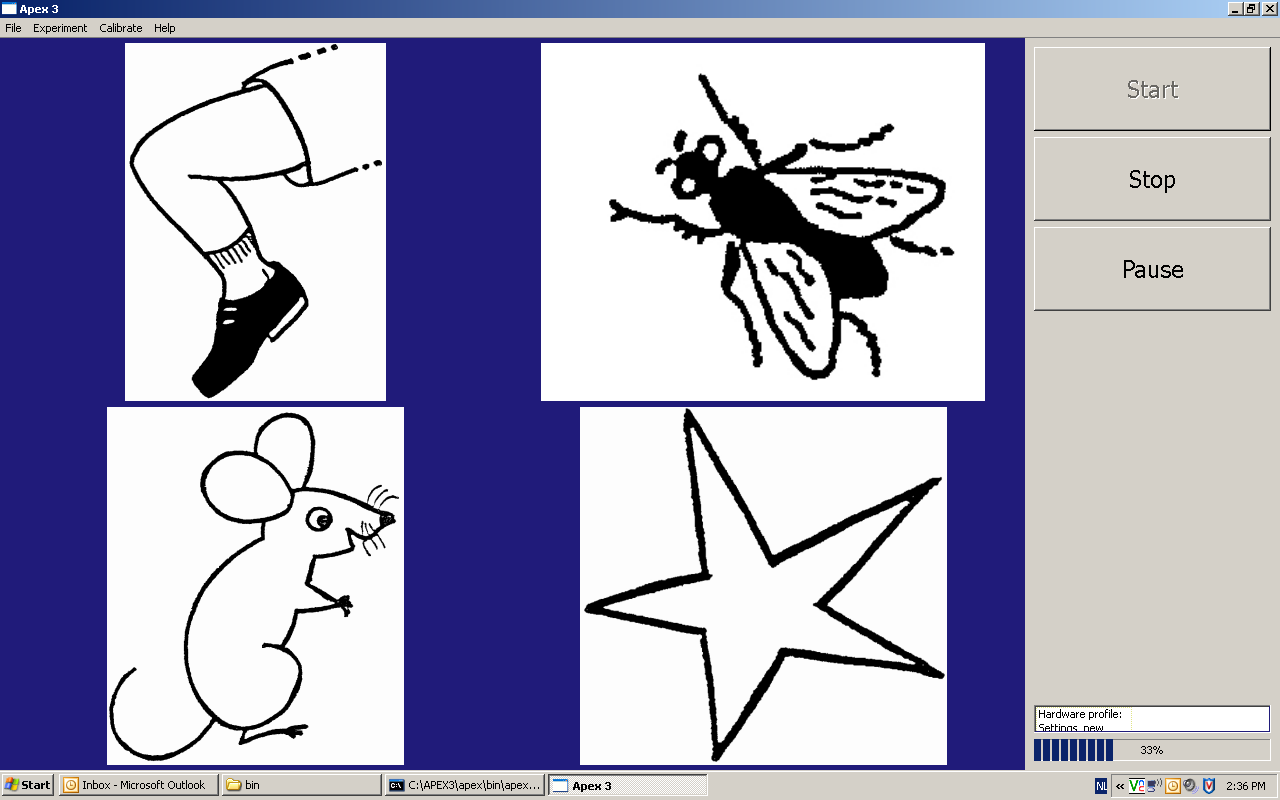
\includegraphics[width=\textwidth]{example1closedset.png}
 \caption{Example of closed-set identification experiment}
 \label{fig:closedset}
\end{figure}

\subsection{Conceptual}
The experiment as described in the previous paragraph should first
be translated to concepts understood by \apex. The main concepts
in this example are \textbf{datablock}, \textbf{stimulus},
\textbf{screen} and \textbf{procedure}. For each of the 3 words to
be presented to the subject, a wave file is available on disk. For
each wave file, a datablock is defined, and for each resulting
datablock a stimulus is defined. Everything that is defined is
assigned an ID, to be able to refer to it later on. Therefore, now
we have 3 stimuli with IDs \id{stimulus_star}, \id{stimulus_mouse}
and \id{stimulus_fly}.

We should also define the things to be shown on the screen during
the experiment. This is done by defining a screen for each word.
Each screen contains 4 pictures, of which one corresponds to the
word. Each screen again gets an ID, in this case we name the
screen by the pictures it contains. Therefore we now have 3
screens with ID \id{screenstar_horse_vase_moon},
\id{screenknee_fly_mouse_star} and \id{screenmouse_fly_star_moon}.

To indicate the order in which the words should be presented, and
together with which screen, a procedure is defined. In the
procedure a number of trials is defined. Recall that a trial is
the combination of a screen, a stimulus and a correct answer.
Therefore a trial is a way to link each of our stimuli with a
screen.

Now only the output logic remains to be defined. The idea is to
continuously present a noise signal and to set the level of the
words such that a certain SNR is obtained. To achieve this, we
define 2 filters, the first one is a generator (i.e., a filter
without input channels) that will generate the noise signal. The
other one is an amplifier, which will amplify or attenuate the
words to obtain the desired SNR.

In the following sections each of the elements of the \xml{XML}
file necessary to implement the latter concepts will be described
in detail. The first one is \element {procedure}.

\subsection{Detailed description of various elements}
\begin{lstlisting}
  <procedure xsi:type="apex:constantProcedureType">
    <parameters>
      <presentations>1</presentations>
      <order>sequential</order>
    </parameters>
    <trials>
      <trial id="trial_star">
        <answer>picturestar</answer>
        <screen id="screenstar_horse_vase_moon"/>
        <stimulus id="stimulus_star"/>
      </trial>
      <trial id="trial_fly">
        <answer>picturefly</answer>
        <screen id="screenknee_fly_mouse_star"/>
        <stimulus id="stimulus_fly"/>
      </trial>
      <trial id="trial_mouse">
        <answer>picturemouse</answer>
        <screen id="screenmouse_fly_star_moon"/>
        <stimulus id="stimulus_mouse"/>
      </trial>
    </trials>
  </procedure>
\end{lstlisting}

The attribute \xml{xsi:type="apex:constantProcedureType"}
indicates that a constant stimuli procedure is used. This means
that the procedure will select the next trial from the trial list
and that it completes after every trial has been presented a
certain number of times.
\begin{itemize}

\item \element{parameters} defines the behavior of the procedure
\begin{itemize}

\item \element{presentations} every trial is presented once

\item \element{order} \xml{sequential} the three trials are
presented sequentially, in the order that is specified in the
experiment file
\end{itemize}
\index{presentations} \index{order}

\item \element{trials} contains different \element{trial} elements
to specify a trial. After selecting a trial the
\element{procedure} will show the specified screen and send the
stimulus to the device. Each trial is given an ID (arbitrary
name), eg \id{TrialStar}, such that it can be referred to later on
or viewed in the results file.

\item \element{answer} the correct answer, to be used by \apex to
determine whether the subject's response is correct. Here, the
subject gets the opportunity to click on one of 4 pictures. The
result from the screen (the subject's response) will be the ID of
the element of the screen that was clicked. Therefore, in this
example, we specify the ID of the picture corresponding to the
stimulus that is presented.
\end{itemize}

A trial must be defined for all the words of the experiment.

\index{trial} \index{answer} \index{screen} \index{stimulus}

\begin{lstlisting}
    <corrector xsi:type="apex:isequal"/>
\end{lstlisting}
\index{corrector}

The corrector checks whether the response is correct or not. The
attribute \xml{xsi:type="apex:isequal"} compares whether the two
input values are exactly the same. In this example
\element{corrector} compares the answer specified under trial and
the ID corresponding to the picture that has been clicked.

\begin{lstlisting}
<screens>
    <uri_prefix>closedset</uri_prefix>
    <reinforcement>
      <progressbar>true</progressbar>
      <feedback length="600">false</feedback>
    </reinforcement>
    <screen id="screenstar_horse_vase_moon">
      <gridLayout height="2" width="2">
        <picture id="picturestar" row="1" col="1">
          <path>star.jpg</path>
        </picture>
        <picture id="picturehorse" row="2" col="1">
          <path>horse.jpg</path>
        </picture>
        <picture id="picturevase" row="1" col="2">
          <path>vase.jpg</path>
        </picture>
        <picture id="picturemoon" row="2" col="2">
          <path>moon.jpg</path>
        </picture>
            </gridLayout>
      <buttongroup id="buttongroup1">
        <button id="picturestar"/>
        <button id="picturehorse"/>
        <button id="picturevase"/>
        <button id="picturemoon"/>
                </buttongroup>
      <default_answer_element>buttongroup1</default_answer_element>
    </screen>
    <screen id="screenknee_fly_mouse_star">
      <gridLayout height="2" width="2">
        <picture id="pictureknee" row="1" col="1">
          <path>knee.jpg</path>
        </picture>
        <picture id="picturefly" row="2" col="1">
          <path>fly.jpg</path>
        </picture>
        <picture id="picturemouse" row="1" col="2">
          <path>mouse.jpg</path>
        </picture>
        <picture id="picturestar" row="2" col="2">
          <path>star.jpg</path>
        </picture>
      </gridLayout>
      <buttongroup id="buttongroup2">
        <button id="pictureknee"/>
        <button id="picturefly"/>
        <button id="picturemouse"/>
        <button id="picturestar"/>
      </buttongroup>
      <default_answer_element>buttongroup2</default_answer_element>
    </screen>
    <screen id="screenmouse_fly_star_moon">
      <gridLayout height="2" width="2">
        <picture id="picturemouse" row="1" col="1">
          <path>mouse.jpg</path>
        </picture>
        <picture id="picturefly" row="2" col="1">
          <path>fly.jpg</path>
        </picture>
        <picture id="picturestar" row="1" col="2">
          <path>star.jpg</path>
        </picture>
        <picture id="picturemoon" row="2" col="2">
          <path>moon.jpg</path>
        </picture>
      </gridLayout>
      <buttongroup id="buttongroup3">
        <button id="picturemouse"/>
        <button id="picturefly"/>
        <button id="picturestar"/>
        <button id="picturemoon"/>
      </buttongroup>
      <default_answer_element>buttongroup3</default_answer_element>
    </screen>
  </screens>
\end{lstlisting}

\element{screens} contains several \element{screen} elements that
can be referred to elsewhere in the experiment file (e.g., in
\element{procedure} above).

\begin{itemize}
\item \element{uri_prefix} a relative path is specified here
(relative with respect to the experiment file). Since \apex knows
the location of the experiment file, only the folder containing
the wave files and pictures must be specified. It is also possible
to give the absolute path, starting at the root. There are 3 ways
to specify a prefix: by directly specifying an absolute path, by
directly specifying a path relative to the experiment file or by
referring to a prefix stored in \filename{apexconfig.xml}. Please
refer to section~\ref{sec:prefixes} for more information.

\item \element{reinforcement} includes

\begin{itemize}

\item \element{progressbar} As the value is \xml{true} a
progressbar will be displayed in the right hand bottom corner of
the screen that indicates how many trials have been completed and
how many remain.

\item \element{feedback length} duration of time after response
(in msec) that \apex waits before presenting the next trial.
During this interval, feedback can be displayed. In this case, no
feedback (thumb up, thumb down) is given as the value is
\xml{false}.

\end{itemize}
\end{itemize}

\begin{itemize}
\item \element{screen} For each word to be presented, a screen is
defined. Each screen has an ID by which it can be referred to
elsewhere in the experiment file (e.g. in \element{trials} to
associate it with a stimulus).
\begin{itemize}

\item \element{gridLayout} specifies how the four figures will be
arranged on the screen. A GridLayout creates a regular grid on the
screen with the specified number of rows and columns. In this
example there are 2 rows and 2 columns. Each figure is defined by
means of a \element{picture} element. Such a definition can be
seen as associating a graphics file with an ID and specifying at
what position of the layout it should be shown. In this case, jpeg
files are used, but other formats are also possible (e.g., png,
bmp, gif).

\begin{itemize}
\item \element{picture}


\element{uri} since the prefix as specified under
\element{uri_prefix} is preprended to each \element {uri}  it
suffices to give the name of the .jpeg file in \element{path}. The
path is relative to the experiment file.

\end{itemize}
\end{itemize}
\begin{itemize}
\item \element{buttongroup} defines a group of screen elements,
namely those (four figures) that are displayed on the screen. The
ID is defined before.

\item \element{default_answer_element} As many elements can be
defined in a screen, \apex has no way to know which element
contains the subject's response. If, for example, a text box is
shown and 2 buttons, it is unclear which is to be used to
determine whether the answer is correct or not. Therefore, in
\element{default_answer_element} the element is designated that
contains the subject's response. In the case of screen elements
that are clicked in order to respond, the example is further
complicated by the fact that we cannot specify just one of the
elements (buttons, pictures), but the response rather comes from a
group of elements. This is when a \element{buttongroup} can be
used to group together different screen elements.
\end{itemize}
\end{itemize}
\index{screens} \index{uri prefix} \index{reinforcement}
\index{progressbar} \index{feedback length} \index{screen}
\index{gridlayout} \index{picture} \index{path}
\index{buttongroup} \index{default answer element}

In this example 5 datablocks are defined, 3 for the word files, 1
for the noise and 1 for silence.

\begin{lstlisting}
 <datablocks>
    <uri_prefix>closedset/</uri_prefix>
    <datablock id="datablock_star">
      <device>wavdevice</device>
      <uri>star.wav</uri>
    </datablock>
    <datablock id="datablock_fly">
      <device>wavdevice</device>
      <uri>fly.wav</uri>
    </datablock>
    <datablock id="datablock_mouse">
      <device>wavdevice</device>
      <uri>mouse.wav</uri>
    </datablock>
    <datablock id="noisedata">
      <device>wavdevice</device>
      <uri>noise.wav</uri>
    </datablock>
    <datablock id="silence">
      <device>wavdevice</device>
      <uri>silence:500</uri>
    </datablock>
  </datablocks>
\end{lstlisting}
\index{datablocks}

\element{datablocks} contains 5 \element{datablock} elements and a
prefix.
\begin{itemize}
\item \element{uri_prefix} a relative path is specified here. It
is also possible to give the absolute path, starting at the root
(see section~\ref{sec:prefixes}).

\item \element{datablock} For each wave file a datablock is made,
with an ID.  \item Each datablock is associated to a
\element{device} (by means of the ID of the device). In datablock
\id{silence} the special syntax is demonstrated for creating a
datablock containing only silence (i.e., all samples are zeros).
This is done to prevent the speech and noise from starting at the
same time. The length of the silence datablock is specified in ms
after the prefix \xml{silence}. It is added before the signal, not
before the noise.

\end{itemize}
\index{datablocks} \index{uri prefix} \index{datablock}
\index{device} \index{uri}

A datablock must be made for all wave files used in the
experiment, including the noise (that will be used by the noise
generator).



In the next sections, the output logic will be defined.
Figure~\ref{fig:ex1-output} gives an overview of the building
blocks that are used in this example. On the left hand side the
datablocks are shown. In the middle the noise generator and the
amplifier and on the right hand side the sound card. As the words
are to be amplified or attenuated according to the desired SNR,
the corresponding datablocks are routed through the amplifier.

\begin{figure}
 \centering
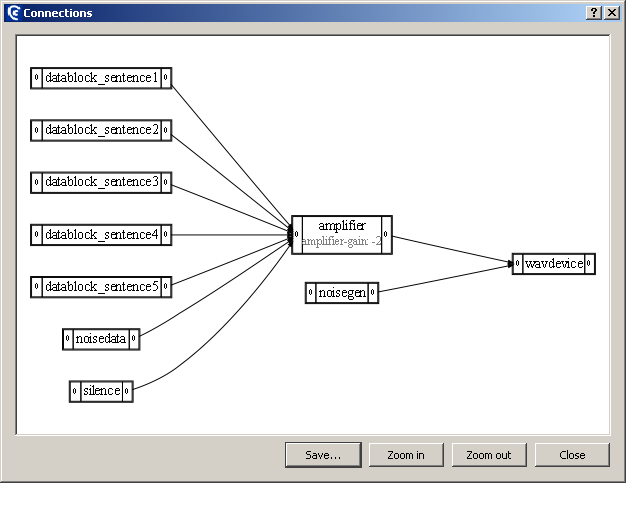
\includegraphics[width=0.5\textwidth]{connectionswindow.png}
 \caption{The connection window}
 \label{fig:ex1-output}
\end{figure}

In the next element the output device is specified.

\begin{lstlisting}
 <devices>
    <device id="wavdevice" xsi:type="apex:wavDeviceType">
      <driver>portaudio</driver>
      <card>default</card>
      <channels>1</channels>
      <samplerate>44100</samplerate>
    </device>
  </devices>

\end{lstlisting}
\index{devices}

All devices defined in the experiment file are grouped in
\element{devices}. In this example there is only 1
\element{device} element. Its ID is set to \id{soundcard}. As an
ID is unique for an entire experiment file, it can be used later
on to refer to this device.

\begin{itemize}
\item  The \xml{xsi:type="apex:wavDeviceType"} attribute tells
\apex that a sound card is used. The experiment only starts if all
devices can be opened.

\item \element{driver} specifies the software driver to be used
for sound output. If unsure, set it to \xml{portaudio}.

\item \element{card} specifies the name of the sound card to be
used. The system default card can be used by specifying
\xml{default} as a card name. Other card names can be defined in
\filename{apexconfig}.

\item \element{channels} specifies the number of channels of the
sound card to be used. The number of channels is restricted to the
selected sound card, with a maximum of 2 for portaudio.

\item \element{samplerate} the sampling rate of the sound card;
Not all sampling rates are supported by all devices, and some
drivers automatically convert the sampling rate. Check your sound
card documentation. The sample rate of the sound card should
correspond to the sampling rates of all datablocks used with it.
If not, an error message will be shown.

\end{itemize}

\index{device} \index{driver} \index{card} \index{channels}
\index{gain} \index{samplerate}

Filters must be defined whenever the signal (or noise) is
manipulated. In this example the level of the noise remains
constant and the signal is amplified or attenuated using an
amplifier filter (loop of \element{datablock}).

\begin{lstlisting}
<filters>
    <filter xsi:type="apex:dataloop" id="noisegen"> (*@\label{xml:filter1}@*)
      <device>wavdevice</device>
      <channels>1</channels>
      <continuous>false</continuous>
      <datablock>noisedata</datablock>
      <basegain>-5</basegain>
      <gain id="noisegain">0</gain>
      <randomjump>true</randomjump>
    </filter>
    <filter xsi:type="apex:amplifier" id="amplifier">  (*@\label{xml:filter2}@*)
      <device>wavdevice</device>
      <channels>1</channels>
      <basegain>-5</basegain>
      <gain id="gain">0</gain>
    </filter>
  </filters>
\end{lstlisting}
\index{filter}

\element{filters} contains individual \element{filter} elements,
which specify a filter, or as a special case a generator (i.e., a
filter without input channels).
\begin{itemize}

\item \element{filter} on line~\ref{xml:filter1} the attribute
\xml{xsi:type="apex:dataloop"} tells \apex that a dataloop
generator has to be created. This is a generator that takes a
datablock and loops it infinitely. The datablock to be looped is
specified by its ID \id{noisedata}. The dataloop generator itself
is assigned the ID \id{noisegen}.


\item \element{filter} on line~\ref{xml:filter2} the attribute
\xml{xsi:type="apex:amplifier"} tells \apex that an amplifier is
to be created. The gain of this amplifier will be varied to change
the amplitude of the words and thus the SNR. It is assigned ID
\id{amplifier}. The gain of the amplifier is made a variable
parameter by assigning it ID \id{gain}
\begin{itemize}
\item \element{device} The device with which the filter is
associated \item \element{channels} The number of channels of the
filter. The available number of channels is dependent on the type
of filter. An amplifier can have any number of channels.

\item If \element{continuous} is set to \xml{true}, the filter or generator
will keep on running in between two trials (i.e., when the subject is responding).
 In this example it stops when the stimulus stops playing (\xml{false}).

\item \element{datablock} The datablock with ID noisedata,
specified under \element{datablocks} will be looped.

\item \element{basegain} the total gain of the amplifier is
basegain+gain. Basegain cannot be a parameter, gain can be a
parameter. The total gain of the complete output system should not
be larger than 0 to avoid clipping of the signal. This is why
basegain = -5.

\item \element{gain} extent to which the signal is amplified.

\item If \element{randomjump} is set to \xml{true}, when the dataloop is started, it will jump to a random sample in the datablock. Thereafter it is looped.
\end{itemize}
\end{itemize}

\index{filters} \index{filter} \index{device} \index{channels}
\index{continuous} \index{datablock} \index{basegain} \index{gain}
\index{randomjump}

\begin{lstlisting}
<stimuli>
    <stimulus id="stimulus_star">
      <datablocks>
        <sequential>
          <datablock id="silence"/>
          <datablock id="datablock_star"/>
          <datablock id="silence"/>
        </sequential>
      </datablocks>
    </stimulus>
    <stimulus id="stimulus_fly">
      <datablocks>
        <sequential>
          <datablock id="silence"/>
          <datablock id="datablock_fly"/>
          <datablock id="silence"/>
        </sequential>
      </datablocks>
    </stimulus>
    <stimulus id="stimulus_mouse">
      <datablocks>
        <sequential>
          <datablock id="silence"/>
          <datablock id="datablock_mouse"/>
          <datablock id="silence"/>
        </sequential>
      </datablocks>
    </stimulus>
  </stimuli>
\end{lstlisting}
\index{stimuli} \index{datablocks}


\element{stimuli} contains different \element{stimulus}, each with
an ID \element{stimulus}

\begin{itemize}\item \element{datablocks}
can be combined in \element{sequential} order (as opposed to
\element{simultaneous}.
\end{itemize}

This is repeated for all the stimuli in the experiment.

\index{stimuli} \index{stimulus} \index{datablocks}
\index{sequential}

\begin{lstlisting}
<connections>
    <connection>
      <from>
        <id>_ALL_</id>
        <channel>0</channel>
      </from>
      <to>
        <id>amplifier</id>
        <channel>0</channel>
      </to>
    </connection>
    <connection>                (*@\label{xml:cha}@*)
      <from>
        <id>amplifier</id>
        <channel>0</channel>
      </from>
      <to>
        <id>wavdevice</id>
        <channel>0</channel>
      </to>
    </connection>               (*@\label{xml:chb}@*)
    <connection>                (*@\label{xml:chc}@*)
      <from>
        <id>noisegen</id>
        <channel>0</channel>
      </from>
      <to>
        <id>wavdevice</id>
        <channel>0</channel>
      </to>
    </connection>               (*@\label{xml:chd}@*)
  </connections>

\end{lstlisting}
\index{connections}

\index{channel}

\element{connections} defines how the different datablocks and
filters are routed to the output device. The ID \id{_ALL_} stands
for all the datablocks. In this example they are routed to the
first channel of the filter with ID {amplifier} (defined under
\element{filters}). In the amplifier the signal is amplified or
attenuated and sent to the wavdevice on lines~\ref{xml:cha}
to~\ref{xml:chb}. At the same time the noise, generated by a
generator with ID noisegen, is sent to the same channel of the
wavdevice. The channels are numbered from 0 onwards. The level of
the noise remains constant and does not pass through an amplifier
(lines~\ref{xml:chc} to~\ref{xml:chd}).

A visual representation of connections can be obtained by choosing
``Show stimulus connections'' under ``Experiment''in the main
\apex menu (top left menu bar).



\begin{lstlisting}
<results>
   <xsltscript>idn.xsl</xsltscript>
</results>
\end{lstlisting}

Even if \element{results} is not specified in the experiment file
\apex will deliver a results file in XML.
\begin{itemize}
\item \element{xsltscript}  a script can transform the XML data to
an easier readable format; this script can be stored in folder
\filename{scripts} under \apex. For more information please read
section~\ref{sec:Using XSLT transforms}.
\end{itemize}
\index{results} \index{xsltscript}

\begin{lstlisting}
<interactive>
   <entry type="int" description="SNR in dB"
    expression="/apex:apex/filters/filter[@id='amplifier']/gain"
    default="0"/>
 </interactive>
\end{lstlisting}

If a small part of an experiment file has to be changed right
before the start of an experiment (e.g. a start value, a gain
value, the subject's name), \apex can show the experimenter a
small \ac{gui} containing the elements to be changed. This is
accomplished by defining the \element{interactive} element in the
experiment file.

In this example we will modify the gain of the filter with ID
\id{amplifier} to a value that is entered by the experimenter at
the start of the experiment.

It is only possible to change the value of an existing element of the experiment file, elements cannot be added. For each element to be changed, an \element{entry} should be defined under \element{interactive}. \element{entry} has  four attributes that should be defined:

\begin{itemize}
\item \attribute{type} specifies the type of input element that
will be shown. If it is \xml{int}, a spinbox\footnote{A spinbox is
an input field that only accepts numbers and has 2 buttons to
respectively increase or decrease its value} will be shown. If it
is \xml{string} a plain text box will be shown. In this case a
spinbox will be shown as a gain is always numeric. \item
\attribute{description} defines the text to be shown in the
\ac{gui} next to the input element, such that the experimenter
knows exactly what to fill in. \item \attribute{expression}
defines the element of the experiment file to be changed. It is
specified by a so-called XPath expression \footnote{see
\url{http://www.w3.org/TR/xpath}}. For a description of XPath, we
refer to the according standard or a good XML book.

\oxygen{OxygenXML can generate XPath expressions for you. First
point the cursor to the target element, then click the right mouse
button and select. An XPath expression to the clicked location is
now in the clipboard and can be pasted at the appropriate place
using the paste function.} \item \attribute{default} specifies the
default value to be shown in the input element.
\end{itemize}

\index{interactive} \index{entry type} \index{expression}

\begin{lstlisting}
<general>
    <showresults>true</showresults>
    <saveprocessedresults>true</saveprocessedresults>
</general>
\end{lstlisting}

\element{general} defines some general parameters. Saving
processed results in a results file is only possible if a
XSLT-script is defined. See section~\ref{sec:Using XSLT
transforms}.

\begin{itemize}
\item \element{showresults} If \xml {true} a window will appear
after completion of the experiment asking whether the results
should be shown on screen.

\item \element{saveprocessedresults} If \xml {true} the
experimenter will be asked whether the processed results must be
appended to the results file.
\end{itemize}

\index{general} \index{showresults} \index{saveprocessedresults}

\newpage
\section{Example 2: Identification of speech in noise using an adaptive method}

\subsection{General description of the experiment}
See \filename{examples/manual/sentenceinnoise.apx}. This is an
example of an adaptive speech in noise test. It determines the
 \ac{srt}, the 50 percent correct point, using
the 1-down, 1-up method described by \citet{PM79}. In this
adaptive procedure the first sentence is repeated with increasing
level until it is identified correctly. Subsequently, the SRT is
determined by increasing or decreasing the level in steps of 2 dB,
according to the last response. Other decision procedures (eg
2-down 1-up) can also be implemented using \apex. In this example
the 5 sentences are scored on the basis of their keywords. The
keywords are indicated in bold on the screen. The
experimenter/clinician is seated in front of the screen and
decides whether the subject has repeated the keywords (of the
sentence) correctly, after which the correct or incorrect button
is clicked(figure~\ref{fig:sentencenoise}). No feedback is
provided. The starting level is given in signal-to noise ratio
(the level of the noise remains the same, that of the signal
varies). In this example speech and noise are routed to the same
channel, i.e. one speaker or one earpiece of the headphone. The
results are written to a results file.

\begin{figure}
 \centering
 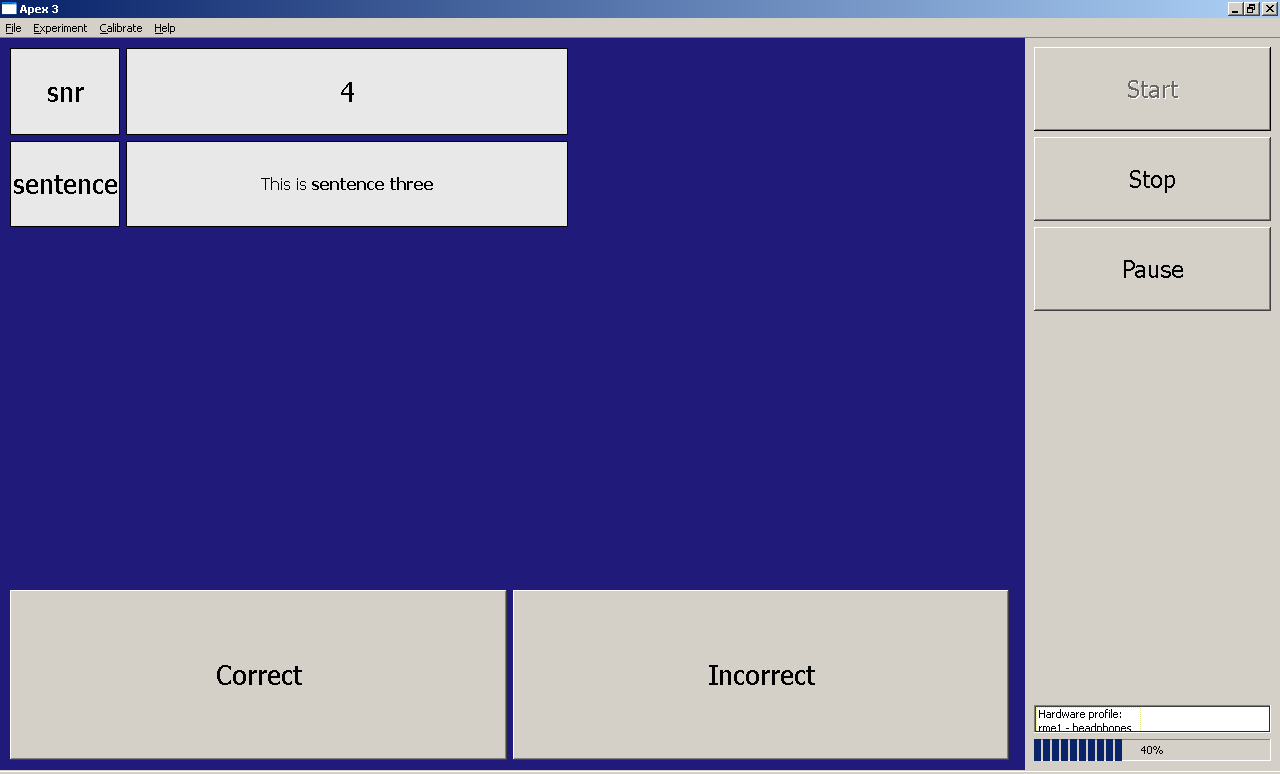
\includegraphics[width=\textwidth]{example2sentenceinnoise.png}
 \caption{Example of adaptive sentence in noise experiment}
 \label{fig:sentencenoise} \todo{bold werkt niet correct?}

\end{figure}
\subsection{Conceptual}
The experiment as described in the previous paragraph should first
be translated to concepts understood by \apex. The main concepts
in this example are \textbf{datablock}, \textbf{stimulus},
\textbf{screen}, \textbf{procedure}, a \textbf{variable} parameter
(to change the gain) and \textbf{fixed Parameter} to show a
sentence on the screen. For each sentence a datablock is defined,
and for each resulting datablock a stimulus is defined. As always,
everything that is defined, is assigned an ID, to be able to refer
to it later on. In this example there are 5 stimuli with IDs
\id{stimulus_sentence1}, \id{stimulus_sentence2},
\id{stimulus_sentence3}, \id{stimulus_sentence4} and
\id{stimulus_sentence5}. The procedure defines a number of trials.
Recall that a trial is the combination of a screen (always the
same in this example), a stimulus and a response.

As we are dealing with an adaptive procedure a fixed or variable
parameter is adapted. In this example a variable parameter is
adapted to change the gain of the sentence, and a fixed parameter
is used to show a sentence on the screen. The screen also shows
the signal-to-noise ratio (SNR) under test and the response
alternatives ``correct'' and ``incorrect''.

Now only the output logic remains to be defined. The idea is to
continuously present a noise signal and to vary the level of the
sentences adaptively. To achieve this, we define 2 filters, the
first one is a generator (i.e., a filter without input channels)
that will generate the noise signal. The other one is an
amplifier, which will amplify or attenuate the sentences to obtain
the desired SNR. Both are connected to one channel of the
wavdevice.

In the following sections each of the elements of the XML file
necessary to implement the latter concepts will be described in
detail.

\subsection{Detailed description of various elements}

\begin{lstlisting}
<procedure xsi:type="apex:adaptiveProcedure">
  <parameters>
    <presentations>1</presentations>
    <order>sequential</order>
    <corrector xsi:type="apex:isequal"/>
    <nUp>1</nUp>
    <nDown>1</nDown>
    <adapt_parameter>gain</adapt_parameter>
    <start_value>0</start_value>
    <stop_after_type>presentations</stop_after_type>
    <stop_after>1</stop_after>
    <larger_is_easier>true</larger_is_easier>
    <repeat_first_until_correct>true</repeat_first_until_correct>
    <stepsizes><stepsize begin="0" size="2"/></stepsizes>
  </parameters>

  <trials>
    <trial id="trial_sentence1">
         <answer>button_correct</answer>
         <screen id="screen"/>
         <stimulus id="stimulus_sentence1"/>
    </trial>

    <trial id="trial_sentence2">
         <answer>button_correct</answer>
         <screen id="screen"/>
         <stimulus id="stimulus_sentence2"/>
    </trial>

    <trial id="trial_sentence3">
        <answer>button_correct</answer>
        <screen id="screen"/>
        <stimulus id="stimulus_sentence3"/>
    </trial>

    <trial id="trial_sentence4">
        <answer>button_correct</answer>
        <screen id="screen"/>
        <stimulus id="stimulus_sentence4"/>
    </trial>

    <trial id="trial_sentence5">
        <answer>button_correct</answer>
        <screen id="screen"/>
        <stimulus id="stimulus_sentence5"/>
    </trial>
  </trials>
</procedure>
\end{lstlisting}


The attribute \xml{xsi:type="adaptiveProcedureType"} of
\element{procedure} refers to a procedure in which a parameter is
changed according to the response of the subject. In this example
the gain of the amplifier is adapted. The procedure selects the
next trial from the trial list and it completes after every trial
has been presented a certain number of times.

\begin{itemize}
\item \element{parameters} defines the behavior of the procedure

\begin{itemize}

\item \element{presentations} every trial is presented once

\item \element{order} the trials are presented sequentially, in
the order that is specified in the experiment file (if
\xml{random} would be specified, they would be presented in random
order).

\item \element{corrector} the corrector checks whether the response is correct or not. The
attribute \xml{xsi:type="apex:isequal"} compares whether the two
input values are exactly the same. In this example
\element{corrector} compares the answer specified under trial  (\id{button_correct}) and
the ID corresponding to the picture that has been clicked (either \id{button_correct} or \id{button_incorrect}).

\item \element{nUp} the level is increased after n (here 1)
incorrect response(s); cf \element{larger_is_easier}

\item \element{nDown} the level is decreased after n (here 1)
correct response(s); cf \element{larger_is_easier}

\item \element{adapt_parameter} to be adapted

\item \element{start_value} the experiment starts with gain=0
(input of user). The value here will be replaced by the entry
value. Please refer to section~\ref{sec:Interactive} for more
information.

\item \element{stop_after_type} the experiment stops after a
specified number of presentations of each trial is completed (it
is also possible to stop after \element{reversals}.

\item \element{stop_after} the experiment stops after 1
presentation of each trial

\item \element{larger_is_easier} If \xml{true}, then larger values
of the parameter are easier than smaller values. It is used to
determine \element{nUp} and \element{nDown}.

\item \element{repeat_first_until_correct} the first trial is
repeated with increasing gain until it is identified correctly.

\item \element{stepsizes} from the beginning of the experiment
(begin=0) the stepsize is 2 dB.
\end{itemize}

\item \element{trials} contains different \element{trial} elements
to specify a trial. Once a trial is selected, \element{procedure}
will show the specified screen and send the stimulus to the
device. Each trial is given an ID (arbitrary name), eg
\id{trialsentence1}, such that it can be referred to later on or
viewed in the results file. A trial must be defined for all the
sentences of the experiment.

\item \element{answer} the correct answer, to be used by \apex to
determine whether the subject's response is correct. In this
example the experimenter will click on ``correct'' or
``incorrect''. The result from the screen will be the ID of the
element of the screen that was clicked (\id{button_correct} or
\id{button_incorrect}).

\end{itemize}

\index{parameters}

\index{procedure}

\index{presentations}

\index{order}

\index{corrector}

\index{nUp}

\index{nDown}

\index{adapt parameter}

\index{start value}

\index{stop after type}

\index{stop after}

\index{larger is easier}

\index{repeat first until}

\index{stepsizes}

\index{trial}

\index{answer}

\begin{lstlisting}
<screens>
        <reinforcement>
            <progressbar>true</progressbar>
            <feedback length="600">false</feedback>
        </reinforcement>

        <screen id="screen">
       <gridLayout height="2" width="1" id="main_layout" rowstretch="1,2">
               <gridLayout width="4" height="4" columnstretch="1,4,2,2"
               rowstretch="1,1,2,2" id="parameter_layout" row="1" col="1">

    <label id="snrlabel" row="1" col="1">
    <text>snr</text>
    </label>

    <parameterlabel id="snr" row="2" col="1">
      <parameter>gain</parameter>
    </parameterlabel>

    <label id="sentence" row="1" col="2">
    <text>sentence</text>
    </label>

    <parameterlabel id="sentence" row="2" col="2">
    <fontsize>12</fontsize>
    <parameter>sentence</parameter>
    </parameterlabel>

    </gridLayout>

    <gridLayout height="1" width="2" id="answer_layout" x="1" y="2">
    <button x="1" y="1" id="button_correct">
    <text>Correct</text>
     </button>
    <button x="2" y="1" id="button_wrong">
    <text>Incorrect</text>
    </button>

    </gridLayout>
    </gridLayout>
    <buttongroup id="buttongroup">
    <button id="button_correct"/>
    <button id="button_wrong"/>
    </buttongroup>
    <default_answer_element>buttongroup</default_answer_element>
    </screen>
    </screens>>
\end{lstlisting}

\element{screens} contains \element{screen} element that is
referred to in \element{procedure}.

\begin{itemize}
\item \element{reinforcement} includes elements on progress and
feedback
\begin{itemize}

\item \element{progressbar} If the value is \xml {true} a progress
bar will be displayed in the right hand bottom corner of the
screen that indicates the percentage of trials that have been completed.

\item \element{feedback length} duration of the time after
response (in msec) that \apex waits before presenting the next
trial. During this interval feedback can be displayed. In this
example, no feedback (thumb up, thumb down) is given as the value
is \xml{false}.
\end{itemize}

\item \element{screen} the screen has an ID by which it can be
referred to in each trial. In this example the screen displays
four blocks in the top left corner to indicate the SNR and the
sentence. In addition, the labels ``Correct'' and ``Incorrect''
are displayed on the buttons at the bottom of the screen (cfr
screenshot, figure...).
\begin{itemize}

\item \element{gridlayout} places elements in an irregular grid.
The screen is divided into sections according to the values. In
this example there are two nested layouts. The main layout divides the screen in two main rows (height = 2, width = 1).
The parameter layout divides the first of these rows in four rows and four columns, of which only the two first ones are filled.
The answer layout divides the second main row in two columns, each with one button.
The stretch factor for the columns is a list of integers, separated by
comma's. There should be as many integers as columns. The width of
the columns is proportional to the numbers. With \xml{width="1"},
and \xml{height="2"} \xml{rowstretch="1,2"} implies that the
second row will be twice as wide as the first one. If
\xml{width="4"}, and \xml{height="4"} and
\xml{columnstretch="1,4,2,2"} the second column will be four times
as wide as the first and two times as wide as the 3rd and 4th.
With \xml{columnstretch="1,1,2,2"} the 3rd and 4th rows will be
twice as wide as the 1st and 2nd.

\item \element{label} the labels on the left are fixed and display
the \element{text} ``SNR'' and ``Sentence''. The button
``Correct'' and ``Incorrect'' are indicated at the bottom of the
screen

\item \element{parameterlabel} the blocks on the right display the values
of the fixed parameters. Gain is the (variable) SNR level, and
sentence is a fixed parameter, defined in \element{stimulus}

\item \element{font size} can be specified in points

\item \element{buttongroup} defines a group of screen elements
(those that are displayed on the screen). As many elements can be
defined in a screen, \apex has no way to know which element
contains the subject's response. Therefore, in
\element{default_answer_element} the element is designated that
contains the subject's response. In the case of screen elements
that are clicked in order to respond, the example is further
complicated by the fact that we cannot specify just one of the
elements (one button, one picture), but that the response rather comes
from a group of elements. This is when a \element{buttongroup} can
be used to group together different screen elements.


\end{itemize}
\end{itemize}
\index{screens} \index{reinforcement} \index{progressbar}
\index{feedback} \index{screen} \index{gridlayout} \index{label}
\index{parameter label} \index{font size} \index{buttongroup}
\index{default answer element}

\begin{lstlisting}
<datablocks>
  <uri_prefix>sentences/</uri_prefix>
  <datablock id="datablock_sentence1">
    <device>wavdevice</device>
    <uri>sent1.wav</uri>
  </datablock>
  <datablock id="datablock_sentence2">
    <device>wavdevice</device>
    <uri>sent2.wav</uri>
  </datablock>
  <datablock id="datablock_sentence3">
    <device>wavdevice</device>
    <uri>sent3.wav</uri>
  </datablock>
  <datablock id="datablock_sentence4">
    <device>wavdevice</device>
    <uri>sent4.wav</uri>
  </datablock>
  <datablock id="datablock_sentence5">
    <device>wavdevice</device>
    <uri>sent5.wav</uri>
  </datablock>
  <datablock id="noisedata">
    <device>wavdevice</device>
    <uri>noise.wav</uri>
  </datablock>
  <datablock id="silence">
    <device>wavdevice</device>
    <uri>silence:500</uri>
  </datablock>
</datablocks>
\end{lstlisting}


\element{datablocks} contains a list of \element{datablock}
elements and a prefix.
\begin{itemize}
\item \element{uri_prefix} a relative path is specified here
(relative with respect to the experiment file). Since \apex knows
the location of the experiment file, only the folder containing
the wave files and pictures must be specified. It is also possible
to give the absolute path, starting at the root. There are 3 ways
to specify a prefix: by directly specifying an absolute path, by
directly specifying a path relative to the experiment file or by
referring to a prefix stored in \filename{apexconfig.xml}. Please
refer to section~\ref{sec:prefixes} for more information. \todo{necessary to repeat all this information here, not enough to refer to prefixes section? (Lot)}

\item \element{datablock} for each wave file a datablock is made,
with an ID.

In datablock \id{silence} the special syntax is
demonstrated for creating a datablock containing only silence
(i.e., zeros). This is done to put silence before and after the
sentence, to prevent the speech and noise from
starting at the same time. The length of the silence datablock is
specified in ms after the prefix \xml{silence}. It is added before the signal (in element \element{stimulus}), not
before the noise.

\begin{itemize}
\item the datablock is associated with the sound card with ID
\id{wavdevice}, as defined in the \element{devices} section.

\item \element{uri} the URI is appended to the prefix defined
above

\end{itemize}
\end{itemize}
\index{uri prefix}

\index{datablocks}

\index{datablock}

\index{device}

\index{uri}


\begin{lstlisting}
<devices>
    <device id="wavdevice" xsi:type="apex:wavDeviceType">
    <driver>portaudio</driver>
    <card>default</card>
    <channels>1</channels>
    <samplerate>44100</samplerate>
    </device>
</devices>
\end{lstlisting}

All devices defined in the experiment file are grouped in
\element{devices}.The ID is set to \id{wavdevice}. As an ID is
unique for an entire experiment file, it can be used later on to
refer to this device (eg in datablocks).

\begin{itemize}
\item \element{device} the \xml{xsi:type="apex:wavDeviceType"}
attribute tells \apex that a sound card is used. The experiment
only starts if all devices can be opened.

\item \element{driver} specifies the software driver to be used
for sound output. If unsure, set it to \xml{portaudio}.

\item \element{card} specifies the name of the sound card to be
used. The system default card can be used by specifying
\xml{default} as a card name. Other card names can be defined in
\filename{apexconfig.xml}.

\item \element{samplerate} the sampling frequency of the sound
card. Not all sampling rates are supported by all devices, and
some drivers automatically convert the sampling rate. Check your
sound card documentation. The sample rate of the sound card should
correspond to the sampling rates of all \element{datablocks} used
with it.
\end{itemize}

\index{device} \index{driver} \index{card} \index{channels}
\index{gain} \index{samplerate}

\begin{lstlisting}
<filters>
<filter xsi:type="apex:dataloop" id="noisegen">
    <device>wavdevice</device>
    <channels>1</channels>
    <continuous>false</continuous>
    <datablock>noisedata</datablock>
    <basegain>-5</basegain>
    <gain>0</gain>
    <randomjump>true</randomjump>
    </filter>
<filter xsi:type="apex:amplifier" id="amplifier" >
    <device>wavdevice</device>
    <channels>1</channels>
    <basegain>-5</basegain>
    <gain id="gain">0</gain>
</filter>
</filters>
\end{lstlisting}

\element{filters} contains individual \element{filter} elements,
which specify a filter, or as a special case a generator (i.e., a
filter without input channels).

\begin{itemize}

\item The attribute \xml{xsi:type="apex:dataloop"} tells \apex
that a dataloop generator has to be created. This is a generator
that takes a datablock and loops it infinitely. The datablock to
be looped is specified by its ID \id {noisedata}.

\item \element{filter} on line~\ref{xml:filter2} the attribute
\xml{xsi:type="apex:amplifier"} tells \apex that an amplifier has
to be created. The gain of this amplifier will be varied to change
the amplitude of the words and thus the SNR. It is assigned ID
\id{amplifier}. The gain of the amplifier is made a variable
parameter by assigning it ID \id{gain}

\begin{itemize}

\item \element{device} the device with which the filter is
associated

\item \element{channels} The number of channels of the filter. The
available number of channels depends on the type of filter. An
amplifier can have any number of channels.

\item \element{continuous} If set to \xml{false} the noise is
presented during the speech, but not during the subject's
response.

\item \element{datablock} the datablock with ID noisedata,
specified under \element{datablocks} will be looped.

\item \element{basegain}:  the total gain of the amplifier is
basegain+gain. The total gain of the complete output system should
not be larger than 0 to avoid clipping of the signal. This is why
basegain = -5.

\item \element{gain} the gain value that is changed. E.g. if the
targetamplitude is 65 dB SPL (see Calibration) the signal and
noise have equal amplitude if gain = 0. Gain is changed by other
modules.

\item If \element{randomjump} is set to \xml{true}, when the
dataloop is started, it will jump to a random sample in the
datablock. Thereafter it is looped.

\end{itemize}

\end{itemize}
\index{filters} \index{filter} \index{device} \index{channels}
\index{continuous} \index{datablock} \index{basegain} \index{gain}
\index{randomjump}

\begin{lstlisting}
<stimuli>
  <fixed_parameters>
    <parameter id="sentence"/>
  </fixed_parameters>

  <stimulus id="stimulus_sentence1">
    <datablocks>
    <sequential>
        <datablock id="silence"/>
        <datablock id="datablock_sentence1"/>
        <datablock id="silence"/>
    </sequential>
    </datablocks>

  <fixedParameters>
    <parameter id="sentence">This is <b> sentence </b> <b>one</b></parameter>
  </fixedParameters>
  </stimulus>

  <stimulus id="stimulus_sentence2">
    <datablocks>
    <sequential>
        <datablock id="silence"/>
        <datablock id="datablock_sentence2"/>
        <datablock id="silence"/>
    </sequential>
    </datablocks>

  <fixedParameters>
    <parameter id="sentence">This is <b> sentence </b> <b>two</b></parameter>
    </fixedParameters> </stimulus>

  <stimulus id="stimulus_sentence3">
    <datablocks>
    <sequential>
        <datablock id="silence"/>
        <datablock id="datablock_sentence3"/>
        <datablock id="silence"/>
    </sequential>
    </datablocks>

<fixedParameters>
<parameter id="sentence">This is <b> sentence </b> <b>three</b></parameter>
</fixedParameters>
</stimulus>

<stimulus id="stimulus_sentence4">
    <datablocks>
    <sequential>
        <datablock id="silence"/>
        <datablock id="datablock_sentence4"/>
        <datablock id="silence"/>
    </sequential>
    </datablocks>

<fixedParameters>
<parameter id="sentence">This is <b> sentence </b> <b>four</b></parameter>
</fixedParameters>
</stimulus>

<stimulus id="stimulus_sentence5">
    <datablocks>
    <sequential>
        <datablock id="silence"/>
        <datablock id="datablock_sentence5"/>
        <datablock id="silence"/>
    </sequential>
    </datablocks>

   <fixedParameters> <parameter id="sentence">This is <b> sentence
   </b> <b>five</b> </parameter> </fixedParameters> </stimulus>
</stimuli>
\end{lstlisting}

\element{stimuli} contains different \element{stimulus}, each with
an ID.

\begin{itemize}
\item \element{fixedParameters} is used here to be able to show
the sentence under test on the Screen. Fixed parameters are
discussed in section~\ref{sec:Parameters}.


\begin{itemize}
\item \element {parameter} the fixed parameter is defined here and
should also be defined in each \element {stimulus}
\end{itemize}

\item \element{stimulus} Each stimulus gets an ID (referred to in
\element {trial})
\begin{itemize}

\item \element{datablocks} here one refers to the
\element{datablock} described before; it includes the sentence
file.

\begin{itemize}
\item \element{sequential} The sequence of \element{datablocks} is
indicated here.
\end{itemize}

\item \element{fixedParameters} sets the fixed parameter for each
\element{stimulus}.

\item \element{b} indicates which words (the keywords) should
appear in bold on screen.
\end{itemize}
\end{itemize}

This is repeated for all the sentences.

\index{stimuli}

\index{fixed parameters}

\index{stimulus}

\index{datablocks}

\index{sequential}

\index{parameter}



\begin{lstlisting}
<connections>
    <connection>
        <from>
        <id>_ALL_</id>
        <channel>0</channel>
        </from>
        <to>
        <id>amplifier</id>
        <channel>0</channel>
        </to>
    </connection>
    <connection>                (*@\label{xml:ch1}@*)
        <from>
        <id>amplifier</id>
        <channel>0</channel>
        </from>
        <to>
        <id>wavdevice</id>
        <channel>0</channel>
        </to>
    </connection>               (*@\label{xml:ch2}@*)
    <connection>                (*@\label{xml:ch3}@*)
        <from>
        <id>noisegen</id>
        <channel>0</channel>
        </from>
        <to>
        <id>wavdevice</id>
        <channel>0</channel>
        </to>
        </connection>           (*@\label{xml:ch4}@*)
</connections>
\end{lstlisting}

\index{connections} \index{channel}

\begin{itemize}
\item \element{connections} defines how the different datablocks
and filters are routed to the output device. The ID \id{_ALL_}
stands for all the datablocks. In this example they are routed to
the first channel of the filter with ID {amplifier} (defined under
\element{filters}). In the amplifier the signal is amplified or
attenuated and sent to the wavdevice on lines~\ref{xml:ch1}
to~\ref{xml:ch2}. At the same time the noise, generated by a
generator with ID noisegen, is sent to the same channel of the
wavdevice. The channels are numbered from 0 onwards. The level of
the noise remains constant and does not pass through an amplifier
(lines~\ref{xml:ch3} to ~\ref{xml:ch4}). Although noisedata is a
\element{datablock} and connected to \emph{amplifier} it is not
specified in \element{stimulus} and does not pass through
\emph{amplifier}.
\end{itemize}

A visual representation of connections can be obtained by choosing
``Show stimulus connections'' under ``Experiment''in the main
\apex menu (top left menu bar).


\begin{lstlisting}
 <results>
  <page>apex:resultsviewer.html</page>
  <resultparameters>
   <parameter name="reversals for mean">4</parameter>
  </resultparameters>
  <showduringexperiment>false</showduringexperiment>
  <showafterexperiment>true</showafterexperiment>
  <saveprocessedresults>true</saveprocessedresults>
 </results>
\end{lstlisting}


\element{results} Even if \element{results} is not specified in
the experiment file \apex will save a results file in XML.

\todo{new part, to check!}
\begin{itemize} 
\item \element{page} URL of the html page to show in the results window. The page should have the appropriate java script methods embedded. More example pages can be found in the \apex resultsviewer folder.
\item \element{resultparameters} Parameters to be passed to the results page. Each parameter will be set in hash params. In this example, the result will be calculated as the mean of the variable parameter (gap) at the last 4 reversals.  \todo{what is hash params? (lot)}
\item \element{showduringexperiment} If true, an extra window will be created which will show the results of the current experiment while the experiment is being executed. Javascript embedded in the page will be executed upon each new trial.
\item \element{showafterexperiment} If true, when the experiment is finished, a dialog box will appear querying whether results should be shown. If the answer is affirmative, a new window will be opened and the results will be shown after javascript processing.
\item \element{saveprocessedresults} If \xml {true} the
experimenter will be asked whether the processed results must be
appended to the results file. This will only work if the results are successfully saved to disk and your javascript code supports this transformation.
\end{itemize}

\index{results} \index{page} \index{resultparameters} \index{showduringexperiment} \index{showafterexperiment} \index{saveprocessedresults}


\begin{lstlisting}
<interactive> <entry type="int" description="SNR start value"
  expression="/apex:apex/procedure/parameters/start_value" default="4" />
</interactive>
\end{lstlisting}

If a small part of an experiment file has to be changed right
before the start of an experiment (e.g. a start value, a gain
value, the subject's name), \apex can show the experimenter a
small \ac{gui} containing the elements to be changed. This is
accomplished by defining the \element{interactive} element in the
experiment file.

In this example we will modify the gain of the filter with ID
\id{amplifier} to a value that is entered by the experimenter at
the start of the experiment.

\begin{itemize}
\item \element{entry type} a value is entered, here corresponding
to SNR in dB. It is also possible to enter a string, e.g. name of
the subject (see Reference Manual).

\item \element{expression} the interactive window will show 4 as
default value; more than one entry may be defined.
\end{itemize}

\index{interactive}

\index{entry type}

\index{expression}

\newpage
\section{Example 3: Gap detection: determining the Just Noticeable Difference}

\todo{example needs modifications, corrector and choices = outdated? modified own version to create new figure }

\subsection{General description of the experiment}
See \filename{examples/manual/gapdetection.apx}. This is an
example of a gap detection task: two stimuli are presented to the
listener in random order, a stationary noise and an interrupted
noise. During the presentation the intervals are highlighted. The
subject's task is to indicate the interval with the
interruption(figure~\ref{fig:gapdetection}). Feedback is provided
(thumb up, thumb down) and the minimal detectable gap is
determined by means of an adaptive procedure (here 2-down, 1-up).
Stimuli (wave files) are generated off line. This example only
includes 5 wave files. Usually many more are generated. The
results are written to a text file.


\begin{figure}
 \centering
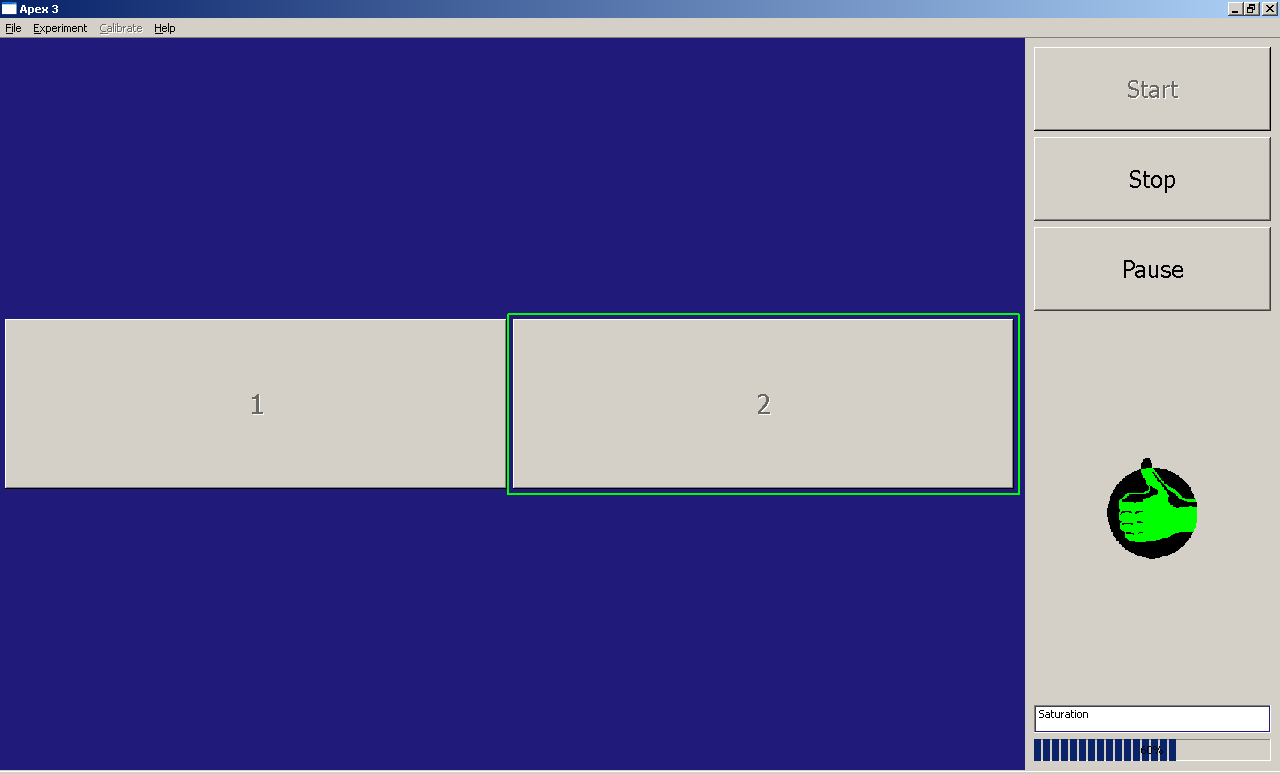
\includegraphics[width=\textwidth]{example3gapdetection.png}
 \caption{Example of adaptive gap detection experiment}
 \label{fig:gapdetection}
\end{figure}

\subsection{Conceptual}
The experiment as described in the previous paragraph should first
be translated to concepts understood by \apex. The main concepts
used here are \textbf{procedure}, \textbf{screens},
\textbf{datablocks} and \textbf{stimuli}.

For each wave file (noise with or without a gap) a \element
{datablocks} is defined, and for each datablock a \element
{stimulus} is defined. In this example there are 5 wave files,
with gap sizes ranging between 1 and 5 ms. Their IDs are
\id{g5ms}, \id{g4ms}, \id{g3ms},\id{g2ms} and \id{g1ms}. In an
adaptive procedure either a fixed or variable parameter is
defined. In this example a fixed parameter is used, i.e. the gap
size in the stimulus. The wave files with different gap sizes are
stored on disk, and are assigned a certain gap value. This gap
value is used to determine the gap threshold. Also, a \element
{screen} is defined that shows the two response intervals
indicating ``1'' and ``2''.

To indicate the order in which the stimuli should be presented a
\element {procedure} is defined. An adaptive procedure is defined
containing 1 \element {trial} with five variable stimuli (with
gap) and the standard stimulus without the gap. Recall that a
\element {trial} is the combination of a \element {screen} (always
the same in this example), a stimulus and a correct answer. The
standard and stimuli occur randomly in one of both intervals.

Now only the output logic remains to be defined. The idea is to
present the standard and a variable stimulus after each other, and
the stimulus to be presented depends on the response of the
subject. Filters are not used since the signals are not changed.

In the following sections each of the elements of the XML file
necessary to implement the latter concepts will be described in
detail.

\subsection{Detailed description of various elements}

\todo{modifications: to check, corrector?}
\begin{lstlisting} 
<procedure xsi:type="apex:adaptiveProcedure">
   <parameters>
     <presentations>1</presentations>
     <order>sequential</order>
     <intervals count="2">
	<interval number="1" element="button1"/>
	<interval number="2" element="button2"/>
	</intervals>
     <pause_between_stimuli>1000</pause_between_stimuli>
     <nUp>1</nUp>
     <nDown>2</nDown>
     <adapt_parameter>gap</adapt_parameter>
     <start_value>5</start_value>
     <stop_after_type>reversals</stop_after_type>
     <stop_after>5</stop_after>
     <min_value>0</min_value>
     <max_value>5</max_value>
     <larger_is_easier>true</larger_is_easier>
     <stepsizes>
       <change_after>reversals</change_after>
       <stepsize  begin="0" size="2"/>
       <stepsize begin="2" size="1"/>
     </stepsizes>
  </parameters>

  <trials>
    <trial id="trial1" >
     <screen id="screen1" />
     <stimulus id="stimulus1" />
     <stimulus id="stimulus2"/>
     <stimulus id="stimulus3"/>
     <stimulus id="stimulus4"/>
     <stimulus id="stimulus5"/>
     <standard id="standard"/>
    </trial>
  </trials>
</procedure>
\end{lstlisting}


\element{procedure} The attribute
\xml{xsi:type="adaptiveProcedureType"} refers to a procedure in which a parameter is changed according to
the response of the subject. In this example 1 trial is defined
with different stimuli from which the adaptive procedure chooses.

\begin{itemize}
\item \element{parameters} defines the behavior of the procedure
(eg., nr of presentations, order of presentation, response
strategy).

\begin{itemize}
\item \element{presentation} every trial is presented once.

\item \element{order} applies to the order of the trials. Since there is only 1
\element{trial}, it does not matter here wether the order is
specified as \element{sequential} or \element{random}.

\item \element{corrector} the corrector checks whether the
response is correct or not. In this example the number of choices
in \element{procedure} was 2. This means that \element{procedure}
will present the target stimulus in either interval 1 or 2.
\element{procedure} informs \element{corrector} about the correct
interval. \element{Corrector} also receives the clicked button from the
screen and looks up the corresponding number in the
\element{interval} element above and compares it with the number it
received from \element{procedure}. \todo{check}

\item \element{alternatives} number of alternatives to choose from
(here: 2 intervals) and the IDs of the buttons (defined under \element{screens} they correspond to.

\item \element{pause_between_stimuli} a pause of 1000 ms will be
introduced between successive wave files;

\item \element{nUp} number of items after incorrect trials to
increase the gap

\item \element{nDown} number of items after correct trials to
decrease the gap

\item \element{min_value} the gap size cannot be smaller than 0.

 \item \element{max_value} the gap size cannot be larger than 5

\item \element{adapt_parameter} the parameter to change, here the
``gap'', see also \element{fixed_parameters}

\item \element{start_value} the gap at which to start, here 5, see
under \element{stimulus}

\item \element{stop_after_type} reversals (it can also stop after
a number of presentations or trials)

\item \element{stop_after} number of reversals after which the
procedure is stopped

\item \element{rev_for_mean} the number of reversals that are used
for the average threshold

\item \element{larger_is_easier} here \xml{true} (the smaller the
gap, the more difficult the task)

\item \element{stepsizes} the stepsize

\end{itemize}

\begin{itemize}
\item\element{change_after} the \element{stepsize} is changed
after a specified number of reversals. In this example a stimulus
is skipped until the second reversal (start at 5, then 3, etc).
Thereafter no stimulus is skipped.

\end{itemize}

\item \element{trials} only 1 trial is defined

\begin{itemize}

\item \element{trial} the ID of the trial

\item\element{screen} the ID of the screen

\item \element{stimulus} the ID of the stimulus

\item \element{standard} the ID of the standard

\end{itemize}
\end{itemize}

\index{parameters}

\index{presentation}

\index{order}

\index{corrector}

\index{alternatives}

\index{pause between stimuli}

\index{nUp}

\index{nDown}

\index{adapt parameter}

\index{start value}

\index{stop after type}

\index{min value}

\index{max value}

\index{larger is easier}

\index{stepsize}

\index{trials}

\index{screen}

\index{stimulus}

\index{standard}



\begin{lstlisting}
<screens>
  <reinforcement>
    <progressbar>true</progressbar>
    <feedback length="300">true</feedback>
    <showcurrent>true</showcurrent>
  </reinforcement>

  <screen id="screen1" >
    <gridLayout height="1" width="2" id="main_layout">
      <button x="1" y="1" id="button1" >
       <text>1</text>
      </button>
      <button x="2" y="1" id="button2" >
       <text>2</text>
      </button>
    </gridLayout>
  <buttongroup id="buttongroup1">
     <button id="button1"/>
     <button id="button2"/>
  </buttongroup>
    <default_answer_element>buttongroup1</default_answer_element>
 </screen>
</screens>
\end{lstlisting}

\begin{itemize}
\item \element{screens} contains several screen elements that can
be referred to elsewhere in the experiment file (e.g. in
\element{procedure} above).


\item \element{reinforcement} includes elements on progress and
feedback

\begin{itemize}

\item \element{progressbar} if \xml {true} a progress bar will be
displayed in the right hand bottom corner of the screen. The
progress bar can indicate the percentage of trials that have been done or it
shows when a reversal occurs in an adaptive procedure. In the
latter case the progress bar will increase at every reversal while
the number of trials varies.

\item \element{feedback length} duration of the time after
response (in msec) that \apex waits before presenting the next
trial. During this interval feedback can be displayed.

\item \element{showcurrent} if \xml{true} the interval is highlighted while a
signal is presented.
\end{itemize}

\item \element{screen} each screen has an ID by which it can be
referred to elsewhere in the experiment. In this example the
screen displays two intervals.

\begin{itemize}


\item \element{gridlayout}places elements in an irregular grid.
The screen is divided into sections according to the values. In
this example there is an equal number of rows (x) and columns (y).

Gridlayout defines a group of screen elements (those that are
displayed on the screen).

\begin{itemize}
\item \element{button} for each interval a button is specified;
this button (interval) displays a number on the screen

\item \element{text} the left interval denotes ``1'', the right
one denotes ``2''.

\end{itemize}

\item \element{buttongroup} defines a group of screen elements
(those that are displayed on the screen). As many elements can be
defined in a screen, \apex has no way to know which element
contains the subject's response. Therefore, in
\element{default_answer_element} the element is designated that
contains the subject's response. In the case of screen elements
that are clicked in order to respond, the example is further
complicated by the fact that we cannot specify just one of the
elements (one button, one picture), but that the response rather comes
from a group of elements. This is when a \element{buttongroup} can
be used to group together different screen elements.

\end{itemize}
\end{itemize}



\index{screens}

\index{reinforcement}

\index{progressbar}

\index{feedback length}

\index{showcurrent}

\index{screen}

\index{gridlayout}

\index{button}

\index{text}

\index{buttongroup}

\index{default answer element}

\begin{lstlisting}
<datablocks>
  <uri_prefix>Gapfiles</uri_prefix>
    <datablock id="g5ms" >
      <device>wavdevice</device>
      <uri>g5.wav</uri>
    </datablock>

    <datablock id="g4ms" >
      <device>wavdevice</device>
      <uri>g4.wav</uri>
    </datablock>

    <datablock id="g3ms"  >
      <device>wavdevice</device>
      <uri>g3.wav</uri>
    </datablock>

    <datablock id="g2ms" >
      <device>wavdevice</device>
      <uri>g2.wav</uri>
    </datablock>

    <datablock id="g1ms"  >
      <device>wavdevice</device>
      <uri>g1.wav</uri>
    </datablock>

    <datablock id="datablockref">
      <device>wavdevice</device>
      <uri>ref500.wav</uri>
    </datablock>
  </datablocks>
\end{lstlisting}


\element{datablocks} contains a list of \element{datablock}
elements and a prefix.

\begin{itemize}
\item \element{uri_prefix}: a relative path is specified here.
Since \apex knows the location of the experiment file, only the
folder containing the wave files and pictures must be specified.



\item \element{datablock} for each wave file a unique datablock is
defined by an ID. The standard signal (uninterrupted noise) must
also be specified here.

\item \element{device} each datablock includes the audio device to
which the signal is routed

\item \element{uri} since the path is defined in
\element{uri_prefix} it is not necessary to specify the entire
path again

\index{datablocks} \index{uri prefix} \index{datablock}
\index{device} \index{uri}

\end{itemize}
\begin{lstlisting}
<devices>
 <device id="wavdevice" xsi:type="apex:wavDeviceType">
 <driver>portaudio</driver>
 <card>default</card>
 <channels>2</channels>
 <gain>0</gain>
 <samplerate>44100</samplerate>
 </device>
</devices>
\end{lstlisting}


\element{devices} all devices defined in the experiment file are
grouped in the \element{devices}. Only 1 \element{device} is used
in this example. The ID is set to soundcard. As an ID is unique
for an entire experiment file, it can be used later on to refer to
this device.

\begin{itemize}
\item \element{device} the \xml{xsi:type="apex:wavDeviceType"}
attribute tells \apex that a sound card is used. The experiment
only starts if all devices can be opened.

\item \element{driver} specifies the software driver to be used
for sound output. If unsure, set it to \xml{portaudio}.

\item \element{card} specifies the name of the sound card to be
used. The system default card can be used by specifying
\xml{default} as a card name. Other card names can be defined in
ApexConfig.

\item \element{channels} 2 channels are specified here, because
the signal is stereo.

\item \element{samplerate} the sampling frequency of the wave
files. Not all sampling rates are supported by all devices, and
some drivers automatically convert the sampling rate. Check your
sound card documentation. The sample rate of the sound card should
correspond to the sampling rates of all datablocks used with it.

\end{itemize}

\index{devices}

\index{driver}

\index{card}

\index{channels}

\index{gain}

\index{samplerate}


\begin{lstlisting}
<stimuli>
   <fixed_parameters>
     <parameter id="gap"/>
   </fixed_parameters>

   <stimulus id="stimulus1" >
     <description>noisewithgap1</description>
     <datablocks>
       <datablock id="g5ms" />
     </datablocks>
     <fixedParameters>
       <parameter id="gap">5</parameter>
     </fixedParameters>
   </stimulus>

   <stimulus id="stimulus2" >
     <description>noisewithgap2</description>
     <datablocks>
       <datablock id="g4ms" />
     </datablocks>
       <fixedParameters>
        <parameter id="gap">4</parameter>
     </fixedParameters>
   </stimulus>

   <stimulus id="stimulus3" >
     <description>noisewithgap3</description>
     <datablocks>
       <datablock id="g3ms" />
     </datablocks>
      <fixedParameters>
       <parameter id="gap">3</parameter>
      </fixedParameters>
   </stimulus>

   <stimulus id="stimulus4" >
     <description>noisewithgap4</description>
     <datablocks>
       <datablock id="g2ms" />
     </datablocks>
       <fixedParameters>
        <parameter id="gap">2</parameter>
       </fixedParameters>
   </stimulus>

   <stimulus id="stimulus5" >
     <description>noisewithgap5</description>
     <datablocks>
       <datablock id="g1ms" />
     </datablocks>
       <fixedParameters>
         <parameter id="gap">1</parameter>
       </fixedParameters>
   </stimulus>

   <stimulus id="standard">
     <datablocks>
      <datablock id="datablockref"/>
     </datablocks>
       <fixedParameters>
        <parameter id="gap">0</parameter>
     </fixedParameters>
   </stimulus>
</stimuli>
\end{lstlisting}


\element{stimuli} defines the auditory events, e.g. noise with gap
and noise without gap.

\begin{itemize}

\item \element{fixedParameters}

\begin{itemize}
\item \element{parameter} the gap is a fixed parameter that is
identified by an ID
\end{itemize}

\item \element{stimulus} this element includes a description of
the (variable) stimulus

\begin{itemize}
\item \element{description}

\item \element{datablocks} the ID refers to the wave file corresponding to the datablock

\item \element{fixedParameter}
\begin{itemize}
\item \element{parameter} includes information on the size of the
variable gap
\end{itemize}

\end{itemize}
\end{itemize}


\index{stimuli}

\index{fixed parameters}

\index{stimulus}

\index{datablocks}

\index{parameter}

\index{standard}

\begin{lstlisting}
<connections>
   <connection>
     <from>
       <id>_ALL_</id>
       <channel>0</channel>
     </from>
     <to>
       <id>wavdevice</id>
       <channel>1</channel>
     </to>
   </connection>

 </connections>
\end{lstlisting}

\index{connections} \index{channel}

\begin{itemize}
\item \element{connections} defines how the different datablocks
and filters are routed to the output device. The ID \id{_ALL_}
stands for all the datablocks. In this example they are routed to
1 channel of the wavdevice.
\end{itemize}

A visual representation of connections can be obtained by choosing
``Show stimulus connections'' under ``Experiment''in the main
\apex menu (top left menu bar).


\begin{lstlisting}
<results>
  <page>apex:resultsviewer.html</page>
  <resultparameters>
   <parameter name="reversals for mean">3</parameter>
  </resultparameters>
  <showduringexperiment>false</showduringexperiment>
  <showafterexperiment>true</showafterexperiment>
  <saveprocessedresults>true</saveprocessedresults>
 </results>
\end{lstlisting}

\element{results} Even if \element{results} is not specified in
the experiment file \apex will save a results file in XML. The results file
will display the correct answers, the reversals, the entire
sequence of responses, and the average threshold based on the
number of reversals and the magnitude of the corresponding gap
parameter specified in the experiment file.

\todo{new part, to check!}
\begin{itemize} 
\item \element{page} URL of the html page to show in the results window. The page should have the appropriate java script methods embedded. More example pages can be found in the \apex resultsviewer folder.
\item \element{resultparameters} Parameters to be passed to the results page. Each parameter will be set in hash params. \todo{perhaps some moren explanation on what this can be and why it is empty here?}
\item \element{showduringexperiment} If \xml{true}, an extra window will be created which will show the results of the current experiment while the experiment is being executed. Javascript embedded in the page will be executed upon each new trial.
\item \element{showafterexperiment} If \xml{true}, when the experiment is finished, a dialog box will appear querying whether results should be shown. If the answer is affirmative, a new window will be opened and the results will be shown after javascript processing.
\item \element{saveprocessedresults} If \xml{true} the
experimenter will be asked whether the processed results must be
appended to the results file. This will only work if the results are successfully saved to disk and your javascript code supports this transformation.
\end{itemize}

\index{results} \index{page} \index{resultparameters} \index{showduringexperiment} \index{showafterexperiment} \index{saveprocessedresults}



\begin{lstlisting}
 <general>
  <exitafter>true</exitafter>
 </general>
\end{lstlisting}

\element{general} defines some general parameters.

\begin{itemize}
\item \element{exitafter} if \xml{true} \apex will close after the experiment has ended and results have been shown.
\end{itemize}

\newpage
\section{Example 4: Gap detection in child mode}

\subsection{General description of the experiment}
See \filename{examples/manual/gapdetectionchild.apx}. This is an
example of a gap detection task adapted to the interest of
children: two stimuli are presented to the listener in random
order, a stationary noise and an interrupted noise. It is the same
experiment as example 3, but pictures (movies) of cars replace
buttons on the screen, and a smiley panel is
shown(figure~\ref{fig:gapchild}). During the presentation of
stimuli the cars are animated. The child's task is to indicate the
stimulus with the interruption. Feedback is provided by smileys
and the minimal detectable gap is determined by means of an
adaptive procedure (here 2-down, 1-up). Only those elements that
are specific to the child mode are described in this example.

\index{Example: gap detection - child mode}

\begin{figure}
 \centering
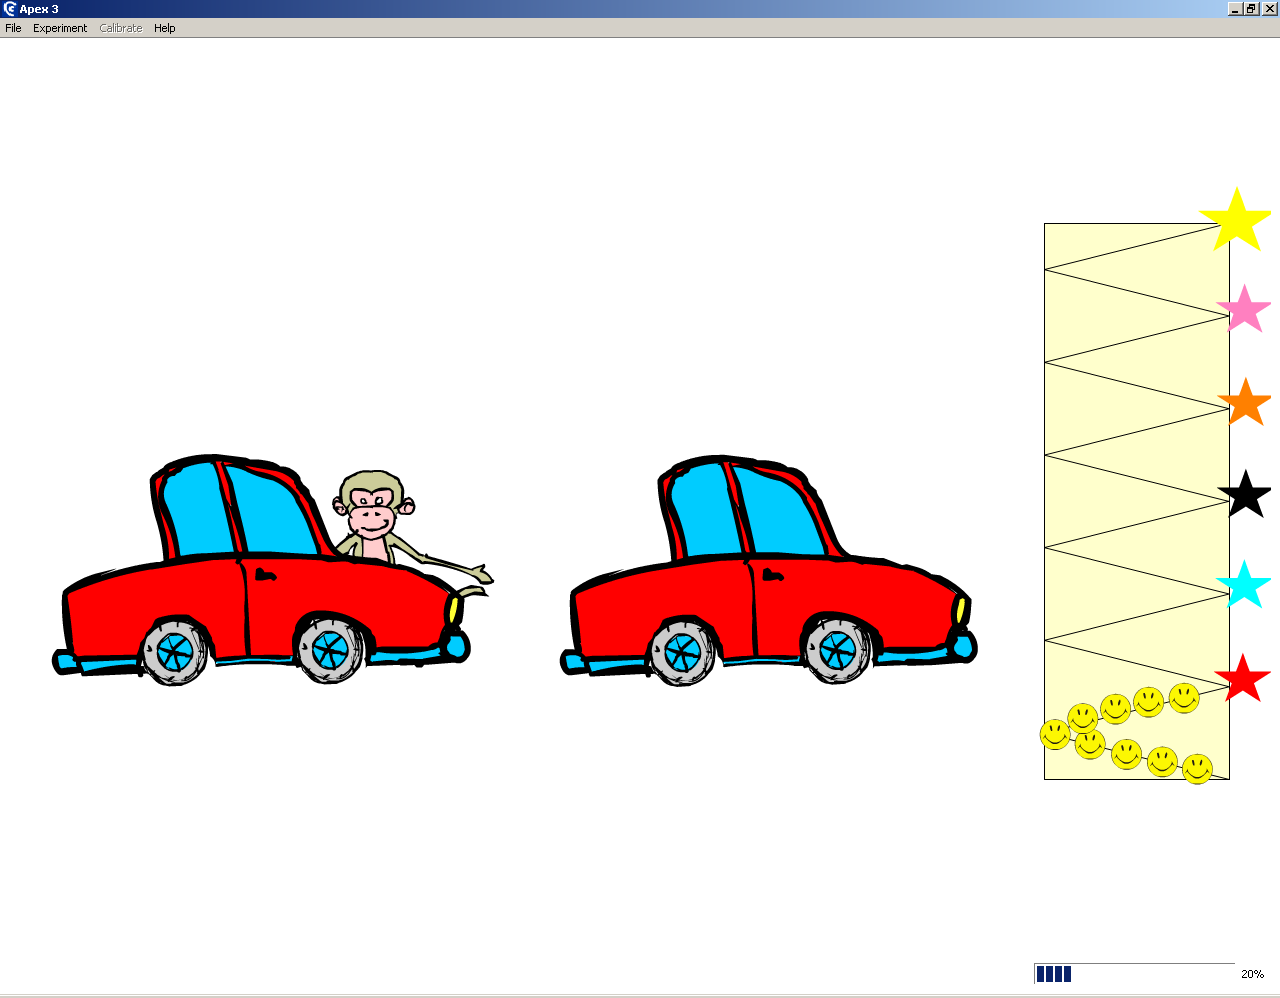
\includegraphics[width=\textwidth]{example4gapdetectionchild.png}
 \caption{Example of gap detection in child mode}
 \label{fig:gapchild}
\end{figure}

\subsection{Conceptual}
The main concepts illustrated in this example are
\textbf{childmode}, and \textbf{reinforcement}. Child mode
involves a different panel, and intro/outro movies.

\subsection{Detailed description of various elements}

\begin{lstlisting}
<screens>
    <uri_prefix>car/</uri_prefix>
    <general>
      <showpanel>true</showpanel>
    </general>
    <reinforcement>
      <progressbar>true</progressbar>
      <feedback length="300">true</feedback>
      <showcurrent>true</showcurrent>
    </reinforcement>
    <childmode>
      <panel>reinforcement.swf</panel>
    </childmode>
    <screen id="screen1">
      <gridLayout height="1" width="2" id="main_layout">
        <flash row="1" col="1" id="button1">
          <path>stillcar.swf</path>
          <feedback>
            <highlight>rijden.swf</highlight>
            <positive>goodcar.swf</positive>
            <negative>badcar.swf</negative>
          </feedback>
        </flash>

        <flash row="1" col="2" id="button2">
          <path>stillcar.swf</path>
          <feedback>
            <highlight>rijden.swf</highlight>
            <positive>goodcar.swf</positive>
            <negative>badcar.swf</negative>
          </feedback>
        </flash>
      </gridLayout>

      <buttongroup id="buttongroup1">
        <button id="button1"/>
        <button id="button2"/>
      </buttongroup>
      <default_answer_element>buttongroup1</default_answer_element>
    </screen>
  </screens>
\end{lstlisting}

\element{screens}

\begin{itemize}
\item \element{uri_prefix} a relative path is specified here
(relative with respect to the experiment file). This only applies
to the movies in \element{screen}. There are 3 ways to specify a
prefix: by directly specifying an absolute path, by directly
specifying a path relative to the experiment file or by referring
to a prefix stored in \filename{apexconfig.xml}. Please refer to
section~\ref{sec:prefixes} for more information.

\item \element{general}

\begin{itemize}

\item \element{show panel} if \xml {true} a panel will be shown
with smileys (see figure \textbf{presented above})

\end{itemize}

\item \element{reinforcement}
\begin{itemize}
\item \element{progressbar} If \xml {true} a progress bar will be
displayed on the right hand side with smileys. The progress bar
shows when a reversal occurs in an adaptive procedure (while the
number of trials varies).

\item \element{feedback length} duration of the time after
response (in msec) that \apex waits before presenting the next
trial. During this interval feedback can be displayed

\item \element{showcurrent} the interval is highlighted while a
signal is presented

\end{itemize}

\item\element{childmode} replaces the ``standard'' panel, sets
some defaults, enables intro/outro movies and changes the
background colour

\begin{itemize}

\item \element{panel} the name of the movie file, per frame
(smileys and panel are a collection of frames)

\end{itemize}

\end{itemize}

\element{screen} Each screen has an ID by which it can be referred
to elsewhere in the experiment. In this example the screen
displays two movies, each containing a car.

\begin{itemize}
\item \element{gridlayout} places elements in an irregular grid.
The screen is divided into sections according to the values. In
this example there are equal number of rows and columns.

\begin{itemize}
\item \element{flash} replaces \element{button} of the standard
version

\begin{itemize}
\item \element{path} the name of the flash movie file on disk,
when there is no animation.

\item \element{feedback}


\item \element{highlight}the name of the file while the car moves

\item \element{positive} the name of the movie file following a
correct response (here a monkey waving)

\item \element{negative} the name of the movie file following an
incorrect response  (the trunk of an elephant)

\end{itemize}

\end{itemize}

\item \element{buttongroup} defines a group of screen elements
(those that are displayed on the screen). As many elements can be
defined in a screen, \apex has no way to know which element
contains the subject's response. Therefore, in
\element{default_answer_element} the element is designated that
contains the subject's response. In the case of screen elements
that are clicked in order to respond, the example is further
complicated by the fact that we cannot specify just one of the
elements (buttons, pictures), but that the response rather comes
from a group of elements. This is when a \element{buttongroup} can
be used to group together different screen elements.


\end{itemize}
\index{screens}

\index{uri prefix}

\index{general}

\index{show panel}

\index{reinforcement}

\index{progressbar}

\index{feedback length}

\index{showcurrent}

\index{childmode}

\index{panel}

\index{screen}

\index{gridlayout}

\index{flash row}

\index{path}

\index{feedback}

\index{highlight}

\index{positive}

\index{negative}

\index{button}

\index{buttongroup}

\index{default answer element}


\incomplete{
\chapter{Example strategies}
\label{chap:Examplestrategies}

\section{N-AFC procedures}

\element{choices}

\index{n-afc procedures}

\section{Roving} \label{sec:roving}

\index{Roving}

randomgenerator

\section{Roving another stimulus dimension}

\section{Identification by typing a sentence}

\index{Open set identification} See
\filename{examples/manual/opensetidentification.apx}. This is an
example of an open set identification task: the subject is
required to type (or repeat) the word or sentence that has been
presented(figure~\ref{fig:opensetidentification}). The results are
written to a text file.

\begin{figure}
 \centering
%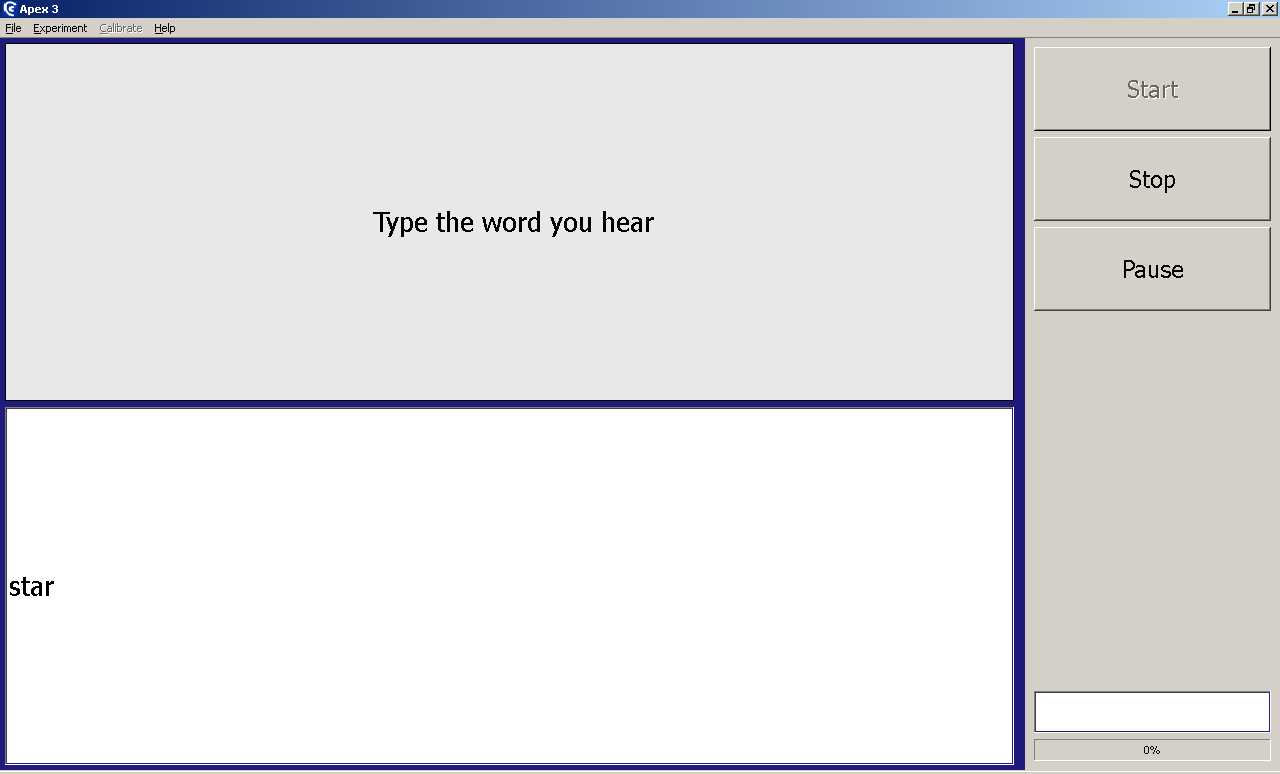
\includegraphics[width=\textwidth]{opensetidentification.png}
 \caption{Example of an open set identification experiment}
 \label{fig:opensetidentification}
\end{figure}

In order to achieve this it is necessary to adapt \element{trial},
\element{answer}, and \element{screens}.


\begin{lstlisting}
  <trial id="trial_maan">
        <answer>moon</answer>
        <screen id="screen"/>
        <stimulus id="stimulus_star"/>
      </trial>
\end{lstlisting}


\begin{lstlisting}
    <screens>
    <reinforcement>
      <progressbar>true</progressbar>
      <feedback length="600">false</feedback>
    </reinforcement>
    <screen id="screen" >
      <gridLayout height="2" width="1" id="main_layout">
        <label x="1" y="1" id="helplabel">
          <text> Type the word you hear</text>
        </label>
        <textEdit x="1" y="2" id="text" >
        </textEdit>
      </gridLayout>
      <default_answer_element>word</default_answer_element>
    </screen>
  </screens>
\end{lstlisting}


\section{Practice}

\index{Practice}

See \filename{examples/manual/trainprocedure.apx}. Here the
subject clicks on an interval and a stimulus is presented. This
can be done as often as he/she wishes.

To achieve this \element{procedure
xsi:type="apex:trainingProcedureType"} should be used.

\section{Higlighting} example threshold
procedure, 2 interval, 1 tone

alle soorten van highlighting (theoretisch deel)

\subsection{Interleaving procedures}

multiprocedure



cmd line parameter


\begin{itemize}
 \item procedure
\item corrector \item ...
\end{itemize}
}
\chapter{Displaying and analysing results}
\label{chap:Results}
\section{The results XML file}
\index{The results XML file}

After completion of the experiment a file containing results is
always given. The default results file is in the XML format and it
contains all the information about the course of the completed
experiment. In the following sections, we see how to display the
results on the screen in a user-friendly format and how to import
them into other software for further analysis.

\apex automatically assigns a default name to the results file,
namely it appends ``-apr'' to the name of the experiment file
(e.g. closedsetword-apr). It will never overwrite an existing
results file, but will append a number to results (e.g.
closedsetword-apr-1) in the case of an existing results file.

The results are stored in the element
\begin{lstlisting}
<apex:results>

</apex:results>
\end{lstlisting}

The XML file contains \element{general} information, such as

\begin{itemize}
\item the testing date

\item the testing duration

\item the name of the XSLT script file (see~\ref{sec:Using XSLT
transforms}).

\item information on the procedure (eg: the adaptive parameter)

\end{itemize}

In addition, for each completed \element{trial} presented to the
subject it includes

\begin{itemize}
\item details of the procedure (stimulus that was presented and
the values of the variable parameters in the specific trial).

\item the response that was chosen by the subject

\item the outcome of the corrector

\item possible errors of the output system/device (eg. underruns)

\item the response time (time between the moment the buttons are
 enabled and the moment an answer is given)


\item in case a random generator was used: the value of the random
generator in the specific trial
\end{itemize}

Remark: with an adaptive procedure the number of
\element{reversals} is given


\section{Displaying results}

APEX has infrastructure to show experiment results on the screen, directly after the experiment, or by opening the results file afterwards with APEX. The system is based on Javascript and HTML, which makes it easy to modify for the end user.

\todo[inline]{explain what HTML is}

In the \xml{<results>} element of the experiment file, you can define the HTML file to be used to display results, e.g.,

\begin{lstlisting}
  <results>
      <page>apex:resultsviewer.html</page>
      <showduringexperiment>true</showduringexperiment>
      <showafterexperiment>true</showafterexperiment>
  </results>
\end{lstlisting}

\xml{<page>} can either refer to a file in the same folder as the experiment file, e.g., \xml{<page>myresults.html</page>}, to a folder somewhere on disk, e.g., \xml{<page>/C/users/tom/myresults.html</page>}, or to a file in the APEX resultsviewer folder, e.g., \xml{<page>apex:specialresultsviewer.html</page>}.

If \xml{<showduringexperiment>} is true, the resultsviewer will be shown while the experiment is running, and will be updated after each trial. If \xml{<showafterexperiment>} is true, it will be shown after the experiment has finished.

\subsection{The results HTML file}

If you want to make small changes to the way results are shown, the best way to start is to copy \filename{resultsviewer.html} to the same folder where your experiment file is stored, rename it something sensible, change the reference in your experiment file, and then modify the HTML file according to the desired result. \todo{give example}

Currently the following divs are available:

\begin{lstlisting}
 <div id="procedureparameterplot" style="width:600px;height:300px;"></div>
   <br>
   <div id="procedureparametervalues"></div>
   <div id="procedureparameterlastvalue"></div>
   <div id="procedureparameterreversals"></div>
   <div id="procedureparametermeanrevs"></div>
   <div id="procedureparametermeantrials"></div>
   <div id="procedureparametertable"></div>


   <div id="confusionmatrixplot"></div>
   <div id="confusionmatrixtable"><table></table></div>
   <div id="confusionmatrixsummary"></div>
\end{lstlisting}
\todo{document each div, automatically extract from resultviewer.html documentation?}

\subsection{The internals - APEX}

If you want to change more than the basic screen layout, you need to change or add some javascript code. In what follows, the internals will be explained. First the APEX side will be explained: how the results viewer gets the actual data from APEX. Next resultsviewer.html and the associated javscript code will be explained.

When results are to be viewed (depending on \xml{<showduringexperiment>} and \xml{<showafterexperiment>}), APEX will load the results HTML file in a basic web browser (called QWebView, based on WebKit). Then, every time a trial is finished, it will call a javascript function \xml{newAnswer}, with as argument a string containing the XML that would normally be written to the results file. For example, after a trial, the following Javascript code cold be executed:


\begin{lstlisting}
	newAnswer("<trial id=\"trial1\">\n<procedure type=\"apex:adaptiveProcedure\">\n<answer>down</answer>\n<correct_answer>up</correct_answer>\n<stimulus>stimulus1</stimulus>\n<correct>false</correct>\n\t<parameter>0</parameter>\n\t<stepsize>2</stepsize>\n\t<reversals>2</reversals>\n\t<saturation>false</saturation>\n\t<presentations>4</presentations>\n</procedure><screenresult>\n\t<element id=\"buttongroup1\">down</element>\n\t<element id=\"down\"></element>\n</screenresult>\n<output>\n<device id=\"wavdevice\">\n  <buffer underruns=\"0\"/>\n</device>\n</output>\n<responsetime unit=\'ms\'>135</responsetime>\n<randomgenerators>\n\n</randomgenerators>\n<trial_start_time>2015-10-22T11:28:15</trial_start_time>\n</trial>\n\n");
\end{lstlisting}

What happens next, fully depends on the HTML/Javascript code.

Whenever new results should be displayed, APEX will call the \xml{plot} function in Javascript. Note that before each plot any number of calls to newAnswer can occur.

\subsection{The internals - \filename{resultsviewer.html}}

The resultsviewer implements the \function{newAnswer} and a number of plotting functions that can be used to display results. In resultsviewer.html itself, the plot() function needs to be implemented, which can refer to any of the plotting functions defined in the provided javascript libraries, e.g., the following code will show a confusion matrix if a constant procedure was used, and a staircase of the adaptive parameter otherwise:

\begin{lstlisting}
<script type="text/javascript">
  $(document).ready(function(){

  });

  function plot() {
    if ( containsAdaptive(results.xml[0])) {
      plot_rtprocedureparameter();
    } else {
      plot_rtconfusionmatrix();
    }
  }
</script>
\end{lstlisting}

\filename{Resultsviewer.html} can include the following javascript libraries:

\begin{description}
\item[rtresults.js] Implements \function{newAnswer} and collects the results in variable \function{results}, which has the following members (all Arrays):
answers, correctanswers, parametervalues, xml, trials, stimuli, standards results \todo{explain each member}. \filename{rtresults.js} does not contain any plotting functions. If you want to do some extra processing when newAnswer is called, you can implement \function{extraNewAnswer}.

\item[rtconfusionmatrix.js] implements \function{plot\_rtconfusionmatrix}, which will calculate and plot a confusion matrix.
\item[rtlocalisation.js] implements \function{plot\_rtlocalisation}, which adds extra functionality on top of \filename{rtconfusionmatrix.js}, specifically for localisation experiments. It will parse the stimulus ID to extract the angle of incidence  (by implementation of \function{extraNewAnswer}), and show extra metrics such as the RMS ans absolute localisation error.
\item[rtprocedureparameter.js] implements \function{plot\_rtprocedureparameter} which will plot the staircase of an adaptive procedure and show a number of performance metrics, such as the mean of the last N trials and of the last N reversals. To set the value of N,  you need to define the variable reversalsForMean, e.g.,
\begin{lstlisting}
\item[rtprocedureparameter.js] implements \function{plot\_rtprocedureparameter} which will plot the staircase of an adaptive procedure and show a number of performance metrics, such as the mean of the last N trials and of the last N reversals. To set the value of N,  you need to define the variable reversalsForMean, e.g.,
\begin{lstlisting}
$(document).ready(function(){
	reversalsForMean=8;}
	);
\end{lstlisting}
}

\item[rtpsignifit.js] implements \function{extraPlot}, which will be automatically called from the plot functions above when this file is loaded. It demonstrates the use of psignifit to estimate psychometric function parameters \citep{Wichmann2001,Wichmann2001a}.

\end{description}

\todo{Add example of how to make a small change}



\section{Exporting results}

While you could simply copy-paste the relevant information from the results XML file into the desired format, this is labour intensive and error prone. Therefore several options are provided to convert the XML file in a more user friendly format.

The first option, \xml{<saveprocessedresults>}, will append a section to the results file containing the essential data in comma separated values (CSV) format, which can be easily copied to another program.

A next option, XSLT transforms, uses the XSLT programming language to convert the results XML file into another format, which could be text, XML, HTML, etc.

If you conduct your analysis in Matlab or R, the most efficient option will be to use the APEX Matlab or R toolbox, and import your result XML file directly. In the R toolbox, a function is also provided to convert a series of results XML files into one main CSV file.

\subsection{saveprocessedresults}


If \element{saveprocessedresults} is \xml{true} in the experiment
file the processed data will be appended to the XML file under
\element{processed}

\todo{add example of output}

The results file contains a lot of information. A summary of the
relevant results can be obtained through an XSLT transform (see
next paragraph).



\subsection{Using the APEX Matlab Toolbox}

\todo{refer to AMT section, add teaser here}

\subsection{Using the APEX R Toolbox}

\todo{}

\subsection{XSLT transforms}

An XSLT script transforms the results XML file to a summary of the
results. An XSLT script is provided with APEX (\filename{apexresult.xsl}), which can do the most common transformations. You can also create your own scripts, provided you have some XSLT knowledge. Please note that we are phasing out the use of XSLT in APEX, in favour of HTML resultsviewer and the APEX Matlab and R toolbox. Therefore the \filename{apexresult.xsl} is no longer maintained, and we advise against using it in new projects.

\label{sec:Using XSLT transforms}

\oxygen{ To execute an XSLT transform, a transformation scenario
has to be configured once. This is done by clicking on the
``Configure transformation scenario'' button in Oxygen. If you
then click on ``new'', you can search for the appropriate XSLT
script in \filename{xslt/} and give it a name in the upper field of the ``edit scenario'' box. If you then
click on ``transform now'', the processed results are shown
immediately.}

The processed results can be saved in the results XML file and/or
shown immediately after a test (in the last case the program asks
whether you want to see them or not).



\appendix

\incomplete{\chapter{Using cochlear implants from Cochlear}
\label{sec:L34}

To directly stimulate subjects using cochlear implants from Cochlear, \apex uses the NICv2 interface, provided by Cochlear.
This interface is abstracted as the L34Device (to be used under \element{devices}).
It is always called L34, irrespective of the device that is used
with NICv2 (which can be an L34 but also an SP12 or other devices).

\section{L34 setup}

To use \apex with the L34 device, you need the L34 plugin, which is provided on request, provided you sign the Cochlear NIC agreement.

After obtaining the L34 plugin (in the form of the file \filename{l34plugin.dll}), copy it to the \filename{plugins} directory under the main APEX directory.
You also need a properly setup Cochlear NICv2 environment. We refer to the NICv2
documentation on how to do this. For \apex it boils down to having
the right version of NICv2 (the same \apex was compiled against)
and having the Nucleus NIC binaries directory in your path. If
this part is setup correctly, you should be able to use the L34
device with device number 0 (the simulated device).

Before starting an \apex experiment that uses the L34device, make sure the appropriate devices are connected to the computer and the NIC environment is setup correctly.


\section{Electrical stimulation files}

When using the L34 device, you need prefined stimulation patterns.
Electrical stimulation patterns are not stored in the wave format, such as for the wavdevice, but as one of the following file types:

\todo{replace qic by aseq}

\begin{description}
\item[qic] In a qic file, 2 parameters are specified per stimulus:
the channel to be used and the magnitude (in \%). Before a qic
file can be sent to the NICv2 interface, it thus first has to be
mapped by apex.
\item[qicext] electrode, magnitude (CU), period, phasewidth, phasegap
\item[xml] defined by cochlear (ref?)
\end{description}

Either of these files can be generated using the Nucleus Matlab Toolbox, provided by cochlear. The most important difference between xml stimulation files and other simulation files, is that for the latter \apex will do channel mapping using a user map defined in the experiment file.

\subsection{Generating .qic files}
In \filename{.qic} files, pulses are defined by a certain magnitude (between 0
and 1) and a channel. They can be generated by the Matlab function
\matlabcmd{genstimulus\_elec.m} and written to disk using the \matlabcmd{save\_sequence.m} function. A .qic file can be read back into matlab using the \matlabcmd{read\_qic.m} function.

As the period is constant for an entire qic file, powerup frames have to be inserted in the file if no stimulation is desired at a certain instant.

\index{Qic files}


\section{Parameters of the L34 device}

To use the L34 device, define a \element{device} under \element{devices}, use the \attribute{xsi:type="apex:L34DeviceType"} attribute.

The L34 device has some main parameters:
\begin{description}
\item[device\_id] The device number to be used, as defined by Cochlear. E.g., the first L34 connected to the computer has id 1. There is a simulated device with id 0, which allows to debug experiments without having an L34 connected. Note that triggering does not work properly with the simulated device.
\item[implant] The implant can be either \xml{cic3} (Esprit3G or Sprint or
Freedom with old internal part) or \xml{cic4} (Freedom with new internal
part).
\end{description}

When using \filename{.qic} or \filename{.qicext} files, \apex calculates the number of current units on the basis of the
defined map. The map can be either entered directly in the experiment file (inline) or
derived from the Nucleus fitting software R126 (fromR126).
The following map parameters should be defined: number of electrodes,
mode, pulsewidth, pulsegap, period (1/total rate) and the C's and
T's for the different channels.

Example:
\begin{lstlisting}
<devices>
 <device id="l34"  xsi:type="apex:L34DeviceType">
    <device_id>1</device_id>
    <implant>cic3</implant>

    <defaultmap>
    <inline>
    <number_electrodes>3</number_electrodes>
    <mode>MP1+2</mode>
    <pulsewidth>25</pulsewidth>
    <pulsegap>8</pulsegap>
    <period>138.9</period>
    <channel number="1" electrode="22" threshold="120" comfort="150"/>
    ...
    <channel number="22" electrode="1" threshold="130" comfort="152"/>
    </inline>
 </defaultmap>
</device>
<devices>
\end{lstlisting}


Note that Cochlear numbers the electrodes from 22 (apex) to 1 (base). You can use either convention in your \filename{.qic} file, as long as the above map is specified correctly.

Note also that when using stimulation files in the XML format, the map is not used.

\index{L34-device}
\index{Implant}
\index{Mode}
\index{Defaultmap}
\index{Inline}
\index{pulsewidth}
\index{Pulsegap}
\index{Period}





\section{Bilateral stimulation}
For bilateral stimulation, two devices with each a map need to be defined.
To control the order of starting both devices, you can specify a master device. If a master device is specified, this will be the last device started. If not specified, the devices are started in order of appearance in the experiment file. The device that sends a trigger signal will typically be the master device.

The \element{trigger} element can be used to specify trigger signals to be sent or received. The \xml{<trigger>out</trigger>} specifies a trigger out signal to be sent and the \xml{<trigger>in</trigger>} tells the device to wait for a trigger signal before starting stimulation.

Example:
\begin{lstlisting}
<master>l34-1</master>
<device id="l34-1"  xsi:type="apex:L34DeviceType">
	<device_id>1</device_id>
	<trigger>out</trigger>
	...
</device>
<device id="l34-2"  xsi:type="apex:L34DeviceType">
	<device_id>2</device_id>
	<trigger>in</trigger>
	...
</device>
\end{lstlisting}


\index{Bilateral stimulation}
\index{L34}

Note that datablocks are attached to a device, and need to be defined twice if they are to be used with both devices.


\index{Master}
\index{Device}
\index{Trigger}
}          % no to be shown in preliminary version
\incomplete{\chapter{Using the Matlab toolbox}

\label{app:Matlab}
}
\incomplete{

\chapter{Plugins}
\label{sec:plugins}

\section{Introduction}
Apex supports custom audio filter plugins. In this way, Apex can easily be extended without modifying Apex itself. A plugin is essentially an object that provides a processing function that accepts a block of samples and returns a processed block of samples.

We will illustrate the process of creating a plugin by implementing an amplifier plugin. Note that Apex already contains an amplifier filter, making this example less useful in practice.

Next to the aforementioned processing function, a filter can also contain parameters. Parameter values can be specified in the experiment xml file or set by another apex module.

\label{sec:plugins}

\section{Solving problems}

using the plugin dialog


\section{Example: amplifier}


\subsection{The experiment file}

Our example amplifier looks as follows in the experiment xml file:

\begin{verbatim}
<filter id="myAmplifier" xsi:type="apex:pluginfilter">
    <device>wavdevice</device>
    <channels>1</channels>
    <continuous>false</continuous>
    <plugin>amplifierplugin</plugin>
    <parameter id="gain" name="gain">-10</parameter>
</filter>
\end{verbatim}

\begin{description}
 \item[plugin] Is the name of the binary plugin file you provide. If no extention is specified, Apex will guess one based on the current operating system.\footnote{On Linux, Apex tries to add the extention \texttt{.so} and the prefix \texttt{lib}. On Windows, Apex tries to add the extention \texttt{.dll}.}
\item[Parameter] is defined for each parameter that the plugin accepts. On initialisation the plugin will be queried for each parameter whether it is valid. The \texttt{id} attribute is the parameter id to be referenced from elsewhere in the experiment file. The name is what the plugin uses to determine which internal parameter to modify.
\end{description}


\subsection{Build environment}

To successfully build a plugin, you need the following things setup properly in your build environment:

\begin{itemize}
 \item A modern compiler, preferably the same as used for compiling Apex\footnote{On Linux we currently use gcc 4.1, on Windows we use Visual studio 2003.}
\item The Qt libraries and build tools \url{http://trolltech.com/developer/downloads/qt/index}
\item The file pluginfilterinterface.h
\item Optional: the amplifier plugin example
\end{itemize}



\subsection{Creating the plugin}

The main steps for creating and using a plugin are:

\begin{itemize}
 \item Create a header file (.h) for your plugin, defining classes inheriting from PluginFilterInterface and PluginFilterCreator. Include pluginfilterinterface.h in this header.
\item Create a source files (.cpp) implementing all methods for your plugin.
\item Create a .pro file for use with qmake to compile your plugin
\item Compile your plugin using qmake and make
\item Copy your plugin library to the Apex plugins directory
\item Create an apex experiment file that refers to your plugin library
\item Run Apex with the experiment file
\end{itemize}
\index{Plugin}

The actual plugin is created by using the file \texttt{pluginfilterinterface.h} and inheriting from the PluginFilterInterface and PluginFilterCreator objects.

The only purpose of the PluginFilterCreator object is to return an instance of your filter. In this way, it is possible to have multiple filters in one library. This is currently not implemented in Apex but only provided in the interface.

The easiest way to implement your own filter, is to start from the amplifier example. We suggest that you use qmake to process a .pro file as follows:

\begin{verbatim}
TEMPLATE = lib

TARGET = amplifierplugin
CONFIG += plugin
CONFIG += debug

QT -= gui

INCLUDEPATH += /path/to/pluginfilterinterface.h

SOURCES += amplifierplugin.cpp
HEADERS += amplifierplugin.h
\end{verbatim}

The most important part about the plugin .h file itself is to inherit from QObject and include the necessary macro's.

\begin{verbatim}
 class AmplifierPluginCreator : public QObject, public PluginFilterCreator
{
    Q_OBJECT
    Q_INTERFACES (PluginFilterCreator)

    ...
\end{verbatim}

In the .cpp file you should include the following:

\begin{verbatim}
Q_EXPORT_PLUGIN2(amplifierplugin, AmplifierPluginCreator)
\end{verbatim}


Then run qmake and make. Make sure that Apex can find your plugin library by putting it in the Apex plugins directory or by providing an absolute or relative path in the experiment xml file.

Note that Apex might crash if your plugin crashes (i.e., overwrites memory it should not, etc.).

If you want to know more about the general plugin mechanism, consult the Qt documentation on QPluginLoader and the Qt Plugin Howto (``The Lower-Level API: Extending Qt Applications'').
}
\incomplete{\chapter{Customizing appearance}
\label{sec:Customizing appearance}

The appearance of virtually every element on the screen can be
customized. On a small scale, every element on screen can be
customized by using tags such as bgcolor or fontsize per element,
but on a broader scale every element can be customized by adding a
style element and specifying a style sheet to be used.

Internally the Qt Stylesheet mechanism is used. For a complete overview on how this works, we refer to the Qt manual, which can also be found on the internet at \url{http://doc.trolltech.com/4.3/stylesheet.html}.

Basically, a style sheet consists of a \emph{selector} and a series of properties that can be set.

\begin{lstlisting}
QPushButton#button1 {
    background-color: red;
}
\end{lstlisting}


Here the selector is on line  1 and the property background-color is set to red.

A selector again consists of two parts: the type of elements that will be affected and the name of the concrete element to select. Here the type is QPushButton and the name is button1. The latter name would be what you specify as an id in the experiment file.

All elements used in Apex are listed in table~\ref{tab:elements}. Several generic names of element are given in table~\ref{tab:names}.

In Apex, stylesheets can be specified at 3 levels: inside the \lstinline!<screens>! element in the \lstinline!<apex_style>! element: if placed here, every element on screen will be affected, including the panel buttons and the main menu. If places in the \lstinline!<style>! element, the stylesheet will affect all screens, but not the panel or menu's. If placed in a specific screen element, only that element will be affected.

\begin{table}
\begin{center}
% use packages: array,booktabs
\begin{tabular}{lll}        \toprule
Element name & Screen element & Description \\      \midrule
QPushButton & button & clickable button \\
QLabel & label & text label \\
& picture & picture  \\
\bottomrule
\end{tabular}
\end{center}
\caption{Screen elements for use in style sheets.}
\label{tab:elements}
\end{table}


\begin{table}
\begin{center}
% use packages: array,booktabs
\begin{tabular}{lll}    \toprule
Name & Type & Description \\ \midrule
background & QWidget & The background of the screen \\
startbutton & QPushButton & The start button \\
\bottomrule
\end{tabular}
\end{center}

\caption{Screen element names for use in style sheets.}
\label{tab:names}
\end{table}


The color names that can be used, are those specified in the css standard. A list can be found at \url{http://www.w3schools.com/css/css_colornames.asp}.
}

\bibliography{apexmanual}


\printindex

\end{document}
